%%
%% This is file `sample-authordraft.tex',
%% generated with the docstrip utility.
%%
%% The original source files were:
%%
%% samples.dtx  (with options: `authordraft')
%% 
%% IMPORTANT NOTICE:
%% 
%% For the copyright see the source file.
%% 
%% Any modified versions of this file must be renamed
%% with new filenames distinct from sample-authordraft.tex.
%% 
%% For distribution of the original source see the terms
%% for copying and modification in the file samples.dtx.
%% 
%% This generated file may be distributed as long as the
%% original source files, as listed above, are part of the
%% same distribution. (The sources need not necessarily be
%% in the same archive or directory.)
%%
%% The first command in your LaTeX source must be the \documentclass command.
\documentclass[sigconf,authordraft,review]{acmart}
%% NOTE that a single column version may be required for 
%% submission and peer review. This can be done by changing
%% the \doucmentclass[...]{acmart} in this template to 
%% \documentclass[manuscript,screen,review]{acmart}
%% 
%% To ensure 100% compatibility, please check the white list of
%% approved LaTeX packages to be used with the Master Article Template at
%% https://www.acm.org/publications/taps/whitelist-of-latex-packages 
%% before creating your document. The white list page provides 
%% information on how to submit additional LaTeX packages for 
%% review and adoption.
%% Fonts used in the template cannot be substituted; margin 
%% adjustments are not allowed.
%%
%% \BibTeX command to typeset BibTeX logo in the docs
\AtBeginDocument{%
  \providecommand\BibTeX{{%
    \normalfont B\kern-0.5em{\scshape i\kern-0.25em b}\kern-0.8em\TeX}}}

%% Rights management information.  This information is sent to you
%% when you complete the rights form.  These commands have SAMPLE
%% values in them; it is your responsibility as an author to replace
%% the commands and values with those provided to you when you
%% complete the rights form.
\setcopyright{acmcopyright}
\copyrightyear{2018}
\acmYear{2018}
\acmDOI{10.1145/1122445.1122456}

%% These commands are for a PROCEEDINGS abstract or paper.
\acmConference[Woodstock '18]{Woodstock '18: ACM Symposium on Neural
  Gaze Detection}{June 03--05, 2018}{Woodstock, NY}
\acmBooktitle{Woodstock '18: ACM Symposium on Neural Gaze Detection,
  June 03--05, 2018, Woodstock, NY}
\acmPrice{15.00}
\acmISBN{978-1-4503-XXXX-X/18/06}


% \usepackage{cite}
% \usepackage{amsmath,amssymb,amsfonts, amsthm}
\usepackage{algorithm, algorithmicx}
\usepackage[noend]{algpseudocode}
\usepackage{graphicx}
\usepackage{textcomp}

% Author defined
% Defined by authors--------------------------------------------
\newtheorem{problem}{Problem}
\newtheorem{lemma}{Lemma}
\newtheorem{theorem}{Theorem}
\newcommand{\Bo}[1]{{\color{red} Bo: #1}}
% \newcommand{\QM}[1]{{\color{blue} QM: #1}}
\newcommand{\QM}[1]{{\color{blue}{#1}}}

\newcommand{\D}{\mathcal{T}}
\newcommand{\V}{\mathsf{V}}
\newcommand{\oR}{\mathcal{R}}
\newcommand{\VV}{\mathtt{V}}
\newcommand{\QQ}{\mathtt{Q}}
\newcommand{\MU}{\mathsf{U}}
\newcommand{\vats}{\mathsf{VQGS}}
\newcommand{\vatss}{\mathsf{VQGS}^+}
\newcommand{\vatssce}{\mathsf{VQGS}^+\mathsf{CE}}
\newcommand{\rand}{\mathsf{Random}}
\newcommand{\full}{\mathsf{Full}}
\newcommand{\avats}{\mathsf{CheetahTraj}}
\newcommand{\cavats}{\mathsf{CheetahTraj}\mathsf{CE}}
\newcommand{\qtavats}{\mathsf{CheetahTraj}-\mathsf{QT}}
\newcommand{\sz}{\textsf{Shenzhen}}
\newcommand{\pt}{\textsf{Porto}}
\newcommand{\cd}{\textsf{Chengdu}}
\newcommand{\prob}{\textsf{QOSP}}
\newcommand{\query}{\mathcal{Q}}
\newcommand{\wpts}{\mathsf{WayPoint}}
\newcommand{\invQ}{\mathsf{InvQuad}}
\newcommand{\II}{\mathcal{I}}

\newcommand{\trim}{\vspace{-2mm}}

\newcommand{\baseline}{\mathsf{baseline}}

\newcommand{\stitle}[1]{\vspace*{0.05em}\noindent{\bf #1:\/}}
\newcommand{\sstitle}[1]{\vspace*{0.05em}\noindent{\bf #1\/.}}

\thispagestyle{plain}
\pagestyle{plain}

\newcommand{\localavats}{\mathsf{local+fix}}

\newcommand{\squishlist}{
	\begin{list}{$\bullet$}
		{ \setlength{\itemsep}{0pt}
			\setlength{\parsep}{3pt}
			\setlength{\topsep}{3pt}
			\setlength{\partopsep}{0pt}
			\setlength{\leftmargin}{1.2em}
			\setlength{\labelwidth}{1em}
			\setlength{\labelsep}{0.6em}
		}
	}
	\newcommand{\squishend}{
	\end{list}
}

%%
%% Submission ID.
%% Use this when submitting an article to a sponsored event. You'll
%% receive a unique submission ID from the organizers
%% of the event, and this ID should be used as the parameter to this command.
%%\acmSubmissionID{123-A56-BU3}

%%
%% The majority of ACM publications use numbered citations and
%% references.  The command \citestyle{authoryear} switches to the
%% "author year" style.
%%
%% If you are preparing content for an event
%% sponsored by ACM SIGGRAPH, you must use the "author year" style of
%% citations and references.
%% Uncommenting
%% the next command will enable that style.
%%\citestyle{acmauthoryear}

%%
%% end of the preamble, start of the body of the document source.
\begin{document}

%%
%% The "title" command has an optional parameter,
%% allowing the author to define a "short title" to be used in page headers.
\title{$\avats$: Quality and Efficiency in Large-scale Trajectory Data Visual Exploration}

%%
%% The "author" command and its associated commands are used to define
%% the authors and their affiliations.
%% Of note is the shared affiliation of the first two authors, and the
%% "authornote" and "authornotemark" commands
%% used to denote shared contribution to the research.

%%\author{Ben Trovato}
%%\authornote{Both authors contributed equally to this research.}
%%\email{trovato@corporation.com}
%%\orcid{1234-5678-9012}
%%\author{G.K.M. Tobin}
%%\authornotemark[1]
%%\email{webmaster@marysville-ohio.com}
%%\affiliation{%
%%  \institution{Institute for Clarity in Documentation}
%%  \streetaddress{P.O. Box 1212}
%%  \city{Dublin}
%%  \state{Ohio}
%%  \country{USA}
%%  \postcode{43017-6221}
%%}

%%\author{Lars Th{\o}rv{\"a}ld}
%%\affiliation{%
%%  \institution{The Th{\o}rv{\"a}ld Group}
%%  \streetaddress{1 Th{\o}rv{\"a}ld Circle}
%%  \city{Hekla}
%%  \country{Iceland}}
%%\email{larst@affiliation.org}


%%
%% By default, the full list of authors will be used in the page
%% headers. Often, this list is too long, and will overlap
%% other information printed in the page headers. This command allows
%% the author to define a more concise list
%% of authors' names for this purpose.
\renewcommand{\shortauthors}{Trovato and Tobin, et al.}

%%
%% The abstract is a short summary of the work to be presented in the
%% article.
\begin{abstract}
Visualizing large-scale trajectory data is a core subroutine for many applications, e.g., traffic management, urban planning, and route recommendation.
However, naively visualizing all trajectories for a target region could result in long delay due to large data volume.
Ad-hoc sampling reduces visualization time but may harm visual quality, i.e., generating visualizations that look substantially different from the exact one.
In this paper, we propose the $\avats$ framework to provide high quality trajectory visualization with low latency.
To this end, we first define a natural pixel-based \textit{visual quality function} to measure the similarity between two visualizations and formulate a quality optimal trajectory sampling problem.
Then, we design the $\vats$ and $\vatss$ algorithms to solve the trajectory sampling problem, which not only provide guaranteed visual quality but also reduce visual clutter.
To generate quality guaranteed trajectory samples with high efficiency, we develop a quad-tree-based index ($\invQ$) that allows to use trajectory samples computed offline.
%Extensive experiments (i.e., case-, user-, and quantitative- studies) are conducted on 3 real-world trajectory datasets to verify visualization quality and efficiency of $\avats$. The results show that $\avats$ consistently provide high quality visualizations and its visualization time is orders of magnitude shorter than visualizing all trajectories.   	
Extensive experiments (i.e., case-, user-, and quantitative- studies) are conducted on 3 real-world trajectory datasets and the results show that $\avats$ consistently provide higher visualization quality and better efficiency than the baselines.  
\end{abstract}

%%
%% The code below is generated by the tool at http://dl.acm.org/ccs.cfm.
%% Please copy and paste the code instead of the example below.
%%
\begin{CCSXML}
<ccs2012>
 <concept>
  <concept_id>10010520.10010553.10010562</concept_id>
  <concept_desc>Computer systems organization~Embedded systems</concept_desc>
  <concept_significance>500</concept_significance>
 </concept>
 <concept>
  <concept_id>10010520.10010575.10010755</concept_id>
  <concept_desc>Computer systems organization~Redundancy</concept_desc>
  <concept_significance>300</concept_significance>
 </concept>
 <concept>
  <concept_id>10010520.10010553.10010554</concept_id>
  <concept_desc>Computer systems organization~Robotics</concept_desc>
  <concept_significance>100</concept_significance>
 </concept>
 <concept>
  <concept_id>10003033.10003083.10003095</concept_id>
  <concept_desc>Networks~Network reliability</concept_desc>
  <concept_significance>100</concept_significance>
 </concept>
</ccs2012>
\end{CCSXML}

\ccsdesc[500]{Computer systems organization~Embedded systems}
\ccsdesc[300]{Computer systems organization~Redundancy}
\ccsdesc{Computer systems organization~Robotics}
\ccsdesc[100]{Networks~Network reliability}

%%
%% Keywords. The author(s) should pick words that accurately describe
%% the work being presented. Separate the keywords with commas.
\keywords{	
Trajectory visualization,
interactive data exploration, sampling}

%% A "teaser" image appears between the author and affiliation
%% information and the body of the document, and typically spans the
%% page.
%% Teaser
 \begin{teaserfigure}
 	\centering
    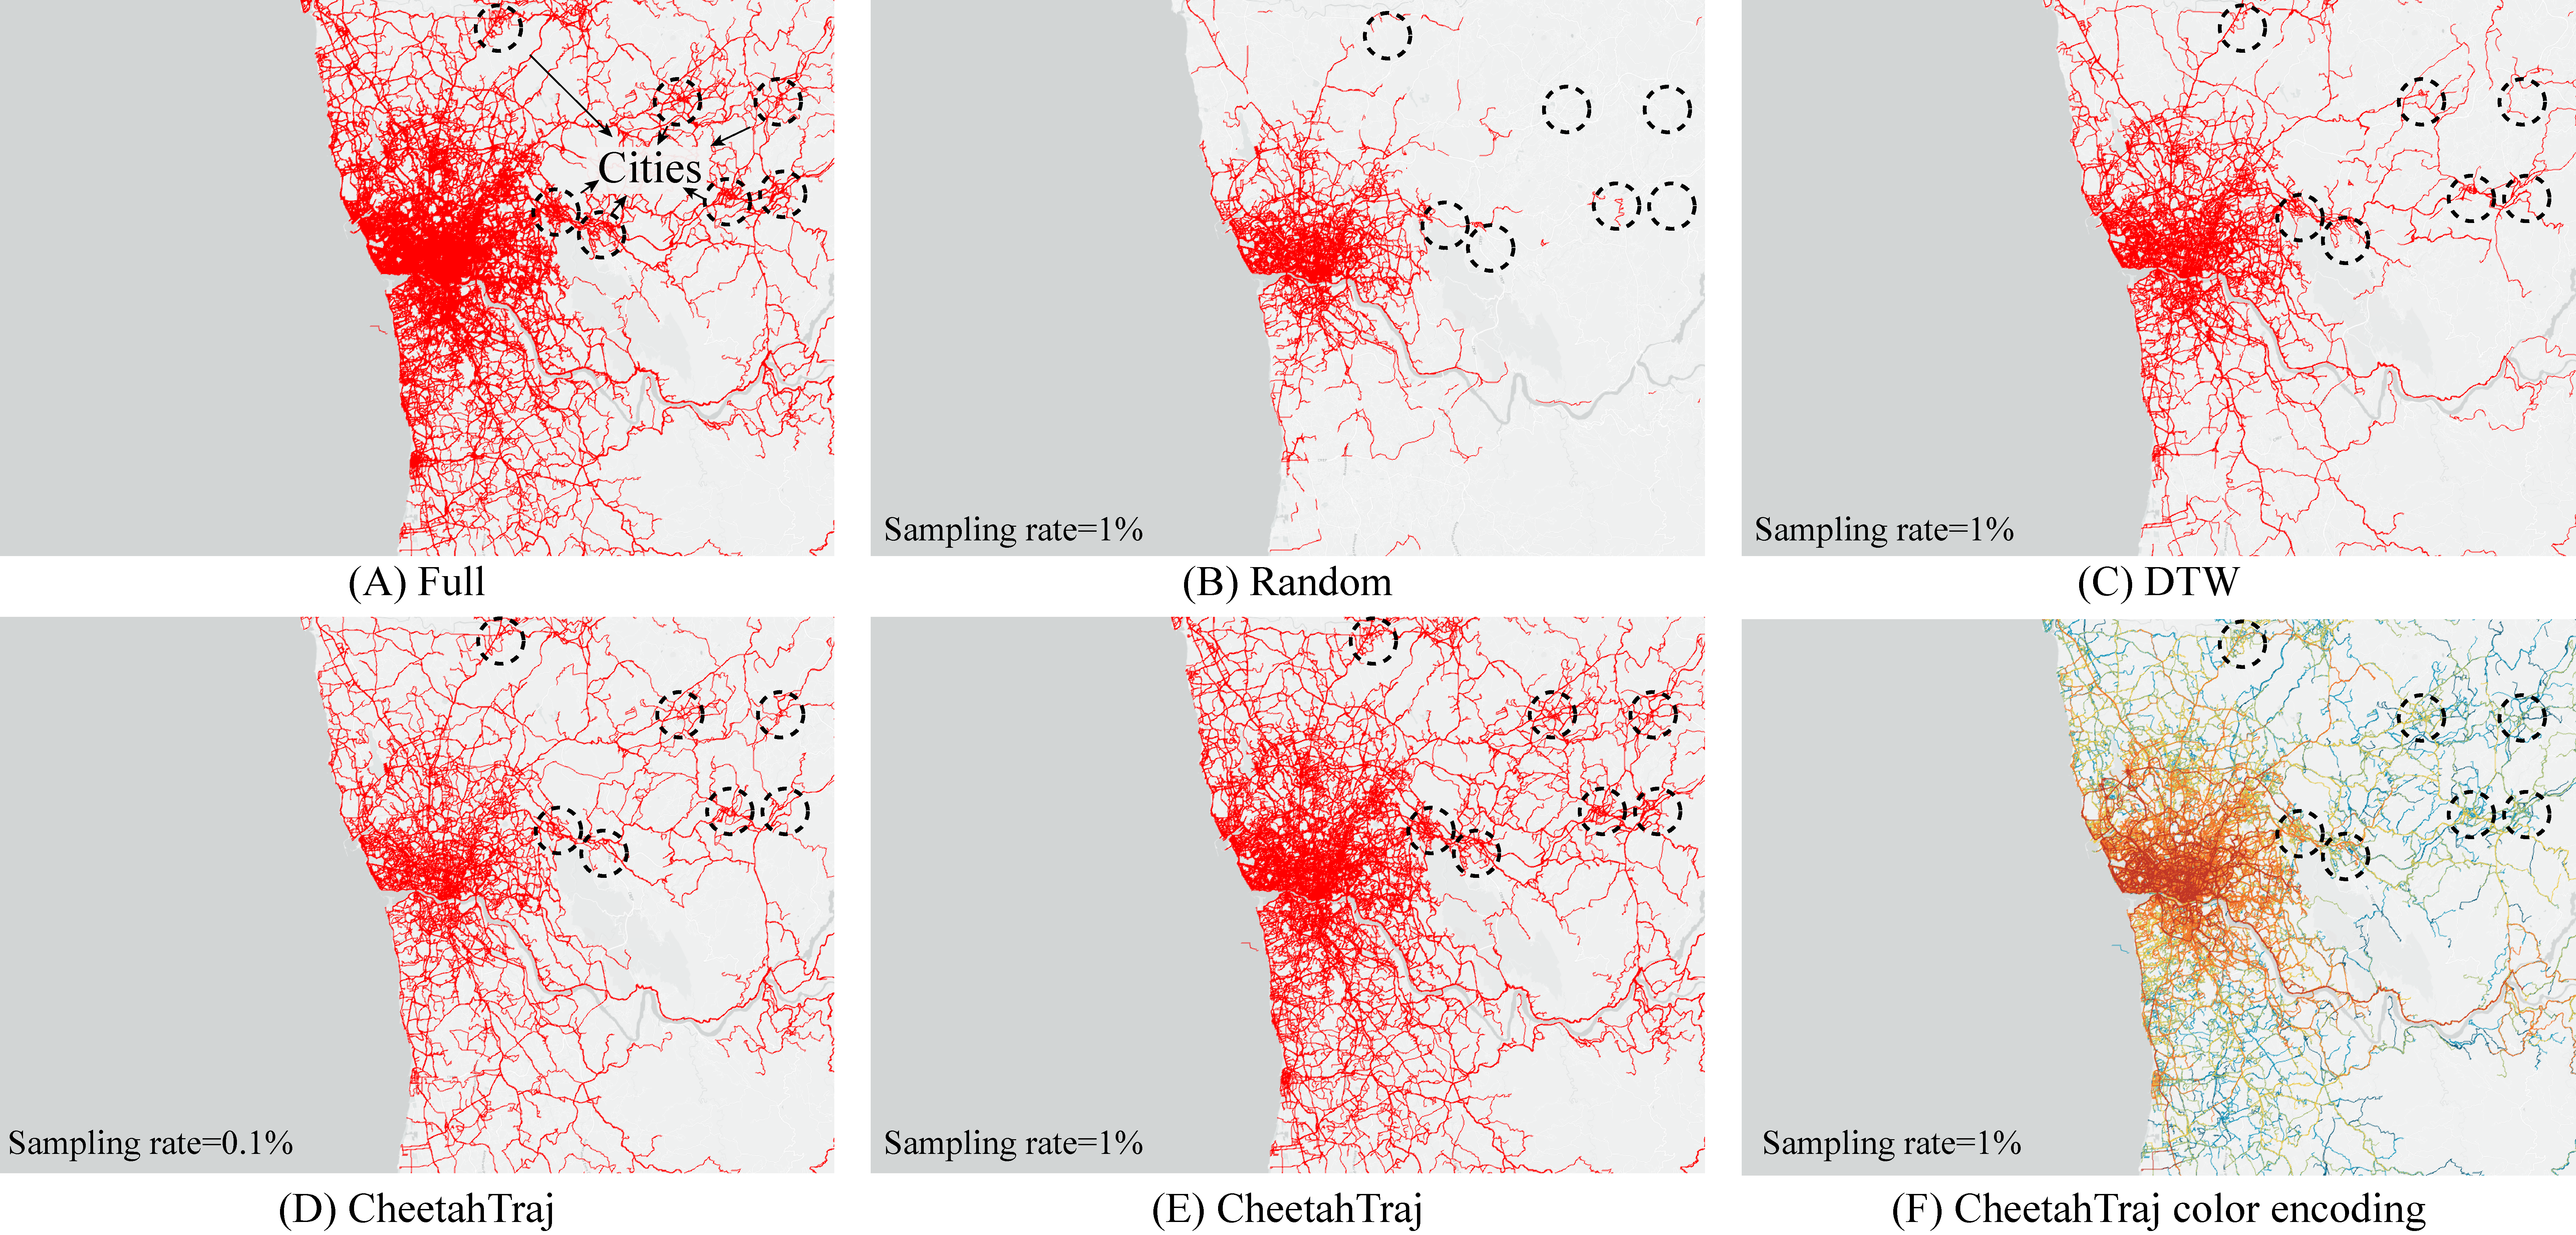
\includegraphics[width=0.82\textwidth]{pictures/case_study_icde/case_study_overview.pdf}
    \vspace{-2mm}
    \caption{Effectiveness of $\avats$ for overview visualization on the \pt{} dataset.}
    \Description{}
    \label{fig:overview}
 \end{teaserfigure}

%%
%% This command processes the author and affiliation and title
%% information and builds the first part of the formatted document.
\maketitle

\section{Introduction}\label{sec:intro}
The ubiquity of location acquisition devices leads to an explosive growth of movement data (i.e., trajectories), e.g., for vehicles, shared bikes and pedestrians. Visualizing these large-scale trajectory data is crucial for many smart city applications~\cite{wang2014visual, tang2017efficient, zheng2011learning} and location-based services~\cite{liu2016smartadp, zheng2010collaborative}. Among various visualization methods, line-based trajectory visualization, which connects the locations of a moving object by polylines, is widely adopted for spatial-temporal data analytics~\cite{chen2015survey, visualanalysis, bigchanvis}. To support interactive exploration on trajectory data, it is crucial to conduct line-based trajectory visualization for an arbitrary region with high quality and low latency.

%\stitle{Long visualization time for large-scale datasets}
\stitle{Challenge for visualizing full datasets} To visualize the trajectories in a target region $\query$, a natural solution is to find the trajectories in it and visualize all these trajectories ($\full$ for short). However, $\full$ may suffer from a long visualization time as the trajectory datasets can be extremely large. For example, Shenzhen has 24,237 taxis which collectively generate more than 7.72 million GPS locations each day~\cite{sz}. Our profiling results in Table~\ref{tab:gpu}\footnote{Mapping is the time to map the GPS points to the screen points, and rendering is the time to render the graphics. The details can be found in Section~\ref{sec:exp}.} also show that visualizing the 1,000,000 taxi trajectories needs 16.154 seconds which is far more than 2 seconds delay suggested for interactive exploration~\cite{shneiderman1984response}.
%However, interactive visual exploration typically requires the visualization to be generated in less than 1 second~\cite{shneiderman1984response}. 
Another problem of applying $\full$ on large-scale datasets is~\textit{visual clutter}~\cite{kwon2017sampling}, where there are too many points in the visualization such that it is difficult for users to gain insights. One such example can be found in Figure~\ref{fig:overview}(A), for which it is difficult to recognize the road networks in the dense center region.   


%We provide an example Figure~\ref{fig:overview}(A) for the \pt{} dataset, for which it is almost impossible to recognize the road networks in the dense region at the center.

\begin{table}
	\centering
	\small
	\caption{Visualization time on the \pt{} dataset (in seconds)}
	\vspace{-2mm}
    \trim
	\begin{tabular}{|c|c|c|c|c|} \hline
		No. of  & No. of & Mapping & Rendering & Total \\
         trajectories &  GPS points & time & time & time \\ \hline
		1,000& 31,300 & 0.027 & 0.003 & 0.03 \\ \hline
		10,000& 31,6531 & 0.169 & 0.005 & 0.174\\ \hline
		100,000& 316,7120 & 1.701 & 0.057 & 1.758 \\ \hline
		1,000,000& 31,646,379 & 15.562 & 0.592 & 16.154 \\ \hline
	\end{tabular}	\label{tab:gpu}
    \trim \trim 
\end{table}

\if 0
\begin{figure*}[t]
	\centering
	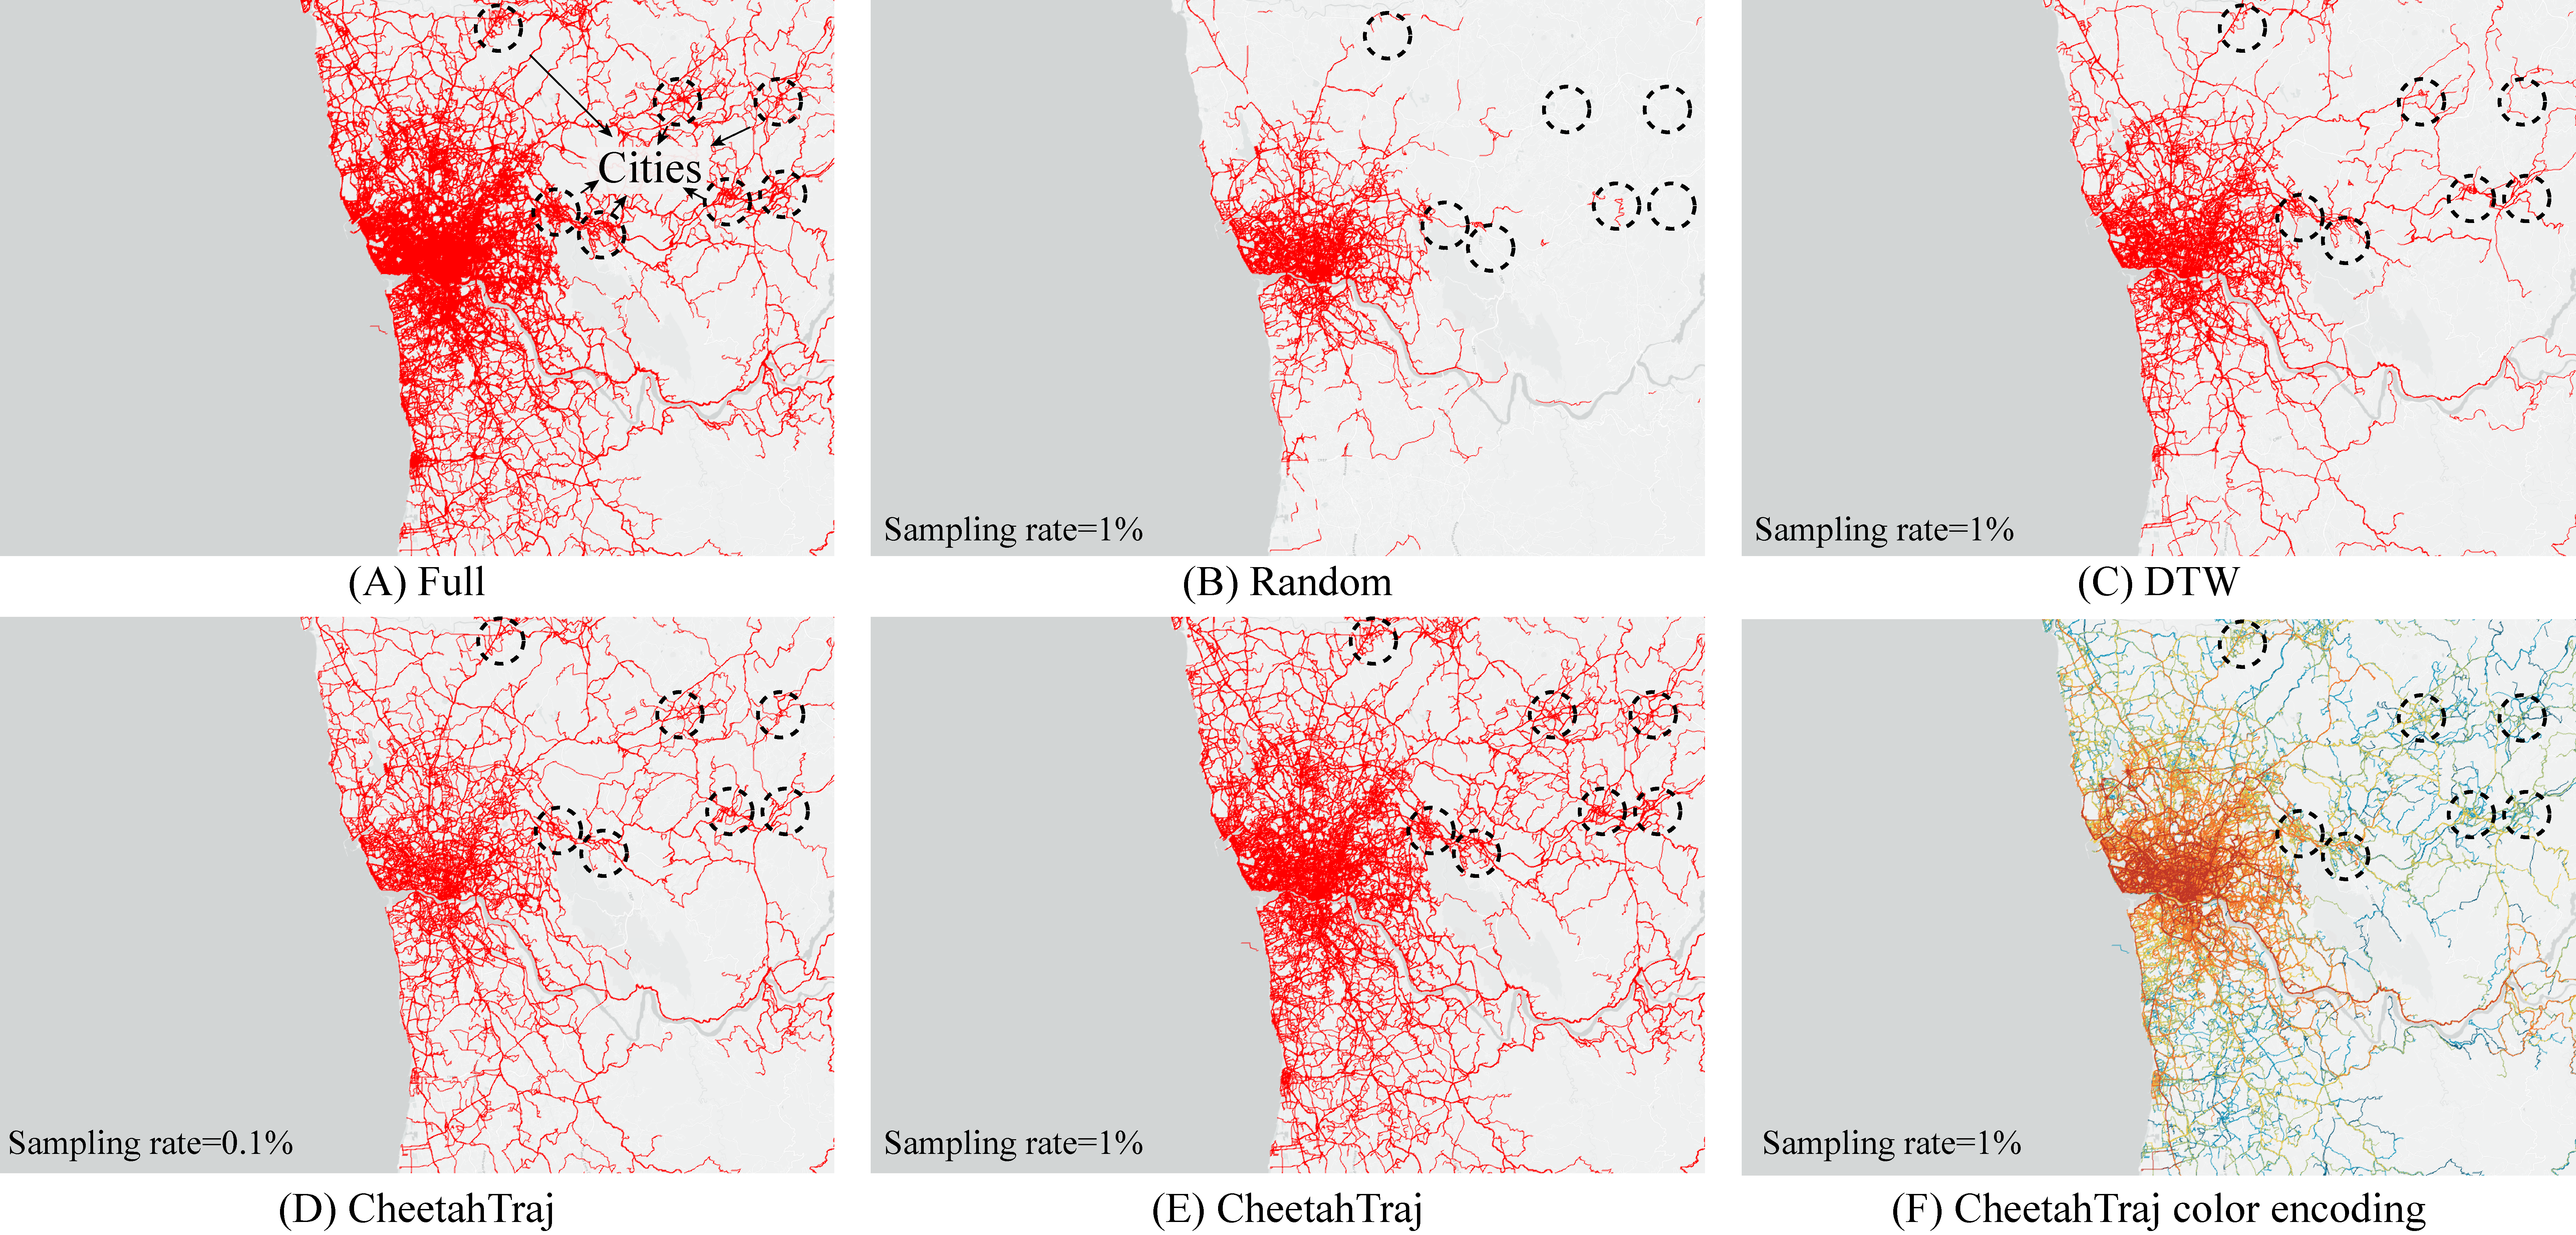
\includegraphics[width=0.75\textwidth]{pictures/case_study_icde/case_study_overview.pdf}
	\trim
	\caption{Effectiveness of $\avats$ at overview visualization in \pt{}.}
	\label{fig:overview}
	\trim \trim
\end{figure*}
\fi
%\stitle{Ad-hoc sampling has poor visual quality} Sampling techniques are widely used to accelerate large-scale data analysis in both database and visualization communities~\cite{qin2020making,DBLP:conf/sigmod/DingHCC016,DBLP:journals/pvldb/KimBPIMR15,park2016visualization}. By selecting a subset of the trajectories in the target region for visualization, sampling can reduce both visualization time and visual clutter. One such example is ScalaR~\cite{battle2013dynamic}, which employs a reduction layer between the visualization layer and the data management layer. The reduction layer samples records \textit{uniformly at random} (denoted as $\rand$) when the query results are too large. However, $\rand$ has poor visual quality as its visualization could be significantly different from the ground-truth. We provide such an example in Figure~\ref{fig:overview}(B), where $\rand$ fails to include trajectories in the sparse areas of Figure~\ref{fig:overview}(A). Another natural idea is to sample trajectories with good diversity and we develop such a baseline using the famous Dynamic Time Warping (DTW) distance between trajectories~\cite{borcan2012improving}. As shown in Figure~\ref{fig:overview}(C), $\mathsf{DTW}$ provides better visualization than $\rand$ but there are still obvious differences between $\mathsf{DTW}$ and the ground-truth in Figure~\ref{fig:overview}(A). Without explicit visual quality guarantee, sampling trajectories in ad-hoc ways may produce visualizations with poor quality and mislead visual exploration.

\stitle{Ad-hoc sampling has poor visual quality} Sampling is widely used to accelerate large-scale data analysis in both information retrieval and data visualization~\cite{qin2020making,DBLP:conf/sigmod/DingHCC016,DBLP:journals/pvldb/KimBPIMR15,park2016visualization}. 
% By selecting a subset of the trajectories in the target region for visualization, sampling can reduce both visualization time and visual clutter. 
One such example is ScalaR~\cite{battle2013dynamic}, which samples records \textit{uniformly at random} (denoted as $\rand$) when the query results are too large. However, $\rand$ has poor visual quality as its visualization can be significantly different from the ground-truth in the sparse areas as shown in Figure~\ref{fig:overview}(B). 
%As shown by Figure~\ref{fig:overview}(B), where $\rand$ fails to include trajectories in the sparse areas of Figure~\ref{fig:overview}(A). 
Another natural idea is to sample trajectories with good diversity and we develop such a baseline using the famous Dynamic Time Warping (DTW) distance between trajectories~\cite{borcan2012improving}. As shown in Figure~\ref{fig:overview}(C), $\mathsf{DTW}$ provides better visualization than $\rand$ but there are still obvious differences between $\mathsf{DTW}$ and the ground-truth in Figure~\ref{fig:overview}(A). 
Without explicit visual quality guarantee, sampling trajectories in ad-hoc ways may produce visualizations with poor quality and mislead visual exploration.


\stitle{The $\avats$ framework} We explore novel algorithm and efficient index jointly in the $\avats$ framework to provide visualizations with high quality and low latency. To conduct quality guaranteed sampling, we first propose a novel pixel-based \textit{visual quality function} to measure how similar an approximate visualization is to the ground-truth. We also show that it is NP-hard to select an optimal set of trajectories that maximize the visual quality function. Next, we devise a \textit{visual quality guaranteed sampling algorithm} named $\vats$, which provides theoretical visual quality guarantee for the sampled trajectories. Then, we \textit{tackle the visual clutter problem} by taking data distribution and human perception into consideration in an advance algorithm named $\vatss$. To avoid running the somehow complex $\vatss$ algorithm on-line for interactive visual exploration, we design an $\invQ$-tree index based on quad-tree, which allows to use the sampling results computed in an offline index building phase. 

%We conducted extensive case study, user study and quantitative performance evaluation to show the effectiveness of $\avats$.

%

%$\invQ$-tree allows to directly use the sampling results computed in an offline index building phase and provides quality guaranteed trajectory samples for an arbitrary target region.

We conduct extensive case study, user study and quantitative performance evaluation to validate the visualization quality and efficiency of the $\avats$ framework. The case study shows that $\avats$ consistently provides high quality visualizations for both large target regions and small target regions. The user study with 35 participants confirms that $\avats$ effectively reduces visual clutter and produces visualizations that are plausible to human inspectors. The quantitative performance evaluation shows that $\avats$ provides good visual quality by sampling only a small number of trajectories. In addition,  $\avats$ produces high quality visualizations for arbitrary target regions in less than 1 second for all 3 experiment datasets and the visualization delay is below 0.1 second in most cases.


We illustrate the merits of our $\avats$ framework in Figure~\ref{fig:overview}. Figure~\ref{fig:overview}(D) and (E) are the visualizations produced by $\avats{}$ on the \pt{} dataset with sampling rate $0.1\%$ and $1\%$, respectively. Compared with uniform random sampling (i.e., $\rand$) and diversity based sampling (i.e., $\mathsf{DTW}$) in Figure~\ref{fig:overview}(B) and (C), Figure~\ref{fig:overview}(D) and (E) are obviously more similar to the full dataset visualization in Figure~\ref{fig:overview}(A).
Figure~\ref{fig:overview}(F) is produced by $\avats{}$ using the same parameters as Figure~\ref{fig:overview}(E) but the trajectories are colored according to their algorithm-generated representativeness (warmer color means more representative). Compared with Figure~\ref{fig:overview}(A), the main routes in the dense region can be identified much more easily, which shows that $\avats{}$ effectively reduces visual clutter. Last but not least, it takes $\avats{}$ only 0.116 seconds and 0.339 seconds to generate Figure~\ref{fig:overview}(D) and (E), respectively, while the full visualization in Figure~\ref{fig:overview}(A) takes 16.154 seconds.



%To sum up, our technical contributions in this paper include:
%
%\squishlist
%  \item We formulate the visual quality optimal trajectory sampling problem for large-scale trajectory data visualization, and prove that it is {NP-hard} (Section~\ref{sec:pro}).
%  \item We devise an approximate algorithm $\vats$ for the visual quality guaranteed sampling problem. $\vats$ is further improved with $\vatss$ by considering data distribution and human perception (Section~\ref{sec:sol}).
%  \item We propose the $\avats$ framework, which jointly uses the aforementioned algorithms and tailored index to achieve both quality and efficiency in large-scale trajectory data visualization (Section~\ref{sec:cheetahtraj}).
%
%\squishend
%
%
%
%This rest of the paper is organized as follows. Section~\ref{sec:rel} introduces related works. The quality optimal trajectory sampling problem is formulated and analyzed in Section~\ref{sec:pro}. Section~\ref{sec:sol} presents our $\vats$ and $\vatss$ algorithm for quality guaranteed trajectory sampling. Section~\ref{sec:cheetahtraj} elaborates the $\avats$ framework. The experiment results are presented in Section~\ref{sec:exp}. Section~\ref{sec:con} draws the conclusions.


\section{Background and Related work}\label{sec:rel}
%In this section, we survey previous work and focus on the most relevant pieces.
%Section~\ref{sec:trajvisana} and ~\ref{sec:interactive} summarize the related works in trajectory visual analysis and interactive data visualization for large dataset, respectively.

In this part, we survey related works on \textit{trajectory visualization methods} in Section~\ref{sec:trajvisana} and \textit{interactive data visualization for large datasets} in Section~\ref{sec:interactive}, respectively.

\subsection{Trajectory Visualization Methods}\label{sec:trajvisana}
A trajectory is a sequence of spatial locations (e.g., GPS positioning results) and trajectories are the most common representations of object movements. Existing trajectory visualization methods can be classified into three categories according to the form of visualization~\cite{chen2015survey}, i.e., \textit{point-based}, \textit{region-based}, and \textit{line-based}. We give a brief introduction to these methods and refer the interested readers to~\cite{chen2015survey} for more detailed discussions.


Point-based visualization plots the locations in the trajectories independently and captures the overall spatial distribution of the moving objects. Many density-based methods~\cite{liu2013vait,yang2016exploring,chae2014public,borruso2008network}, 
%~\cite{liu2013vait,yang2016exploring,chae2014public,xie2008kernel, borruso2008network}
e.g., kernel density estimation, are applied in point-based visualization to preserve the spatial distribution. Region-based visualization slices the entire region into sub-regions and visualizes the aggregated information in each sub-region~\cite{guo2009flow,von2015mobilitygraphs}.
%~\cite{guo2009flow,wood2010visualisation,von2015mobilitygraphs}
As region-based visualization focuses on aggregated statistics, it is most effective in capturing macro-patterns. In this work, we focus on line-based visualization, which uses polylines to connect the locations in each trajectory and shows the trace of object movements (see an example in Figure~\ref{fig:line}). As line-based visualization preserves the continuous movement information of objects~\cite{guo2011tripvista,hurter2009fromdady}, it is widely used in many visual analysis applications such as traffic management, urban planning, and route recommendation. However, line-based visualization is known to suffer from severe visual clutter, especially when the dataset is large. Several techniques have been proposed to alleviate visual clutter, such as clustering-based techniques~\cite{von2015mobilitygraphs}
%~\cite{ferreira2013vector, rinzivillo2008visually, von2015mobilitygraphs}
and advanced interaction techniques~\cite{ferreira2013visual}.
%~\cite{kruger2013trajectorylenses, ferreira2013visual}



\subsection{Interactive Visualization for Large Datasets}\label{sec:interactive}


Figure~\ref{fig:sys_framework} illustrates a general architecture of interactive visualization systems,
e.g., Spotfire\footnote{\url{https://www.tibco.com/products/tibco-spotfire}}, Tableau\footnote{\url{https://www.tableau.com/}}, ATLAS~\cite{chan2008maintaining}, Viate~\cite{yang2019vaite} and Marviq~\cite{dong2020marviq}.
There are typically three layers: user interface in the front-end layer, optimization techniques in the middle-layer, and database management system (usually cloud-based) in the back-end layer. The visualization community usually focuses on improving the effectiveness of data visualization at the front-end, e.g., designing novel visualization methods/toolkits such as D3\footnote{\url{https://d3js.org/}} to enable data analysts to effectively gain insights from data. 
The database community usually aims to improve query efficiency, e.g., devising big data systems such as Spark\footnote{\url{https://spark.apache.org/}} for efficient data processing at the back-end. 
With the popularization of location-acquisition devices, the scale of trajectory datasets can be extremely large. For example, the taxis in Shenzhen generate {$\sim$}9.3GB trajectory data per day. However, visualization generation has a long latency for large datasets due to heavy data processing/graphic rendering, which harms the responsiveness of interactive visualization. Therefore, both the visualization and database communities began to advance techniques in the middle-layer to reduce visualization latency for large datasets. We briefly elaborate these techniques as follows.


\begin{figure}
	\centering
	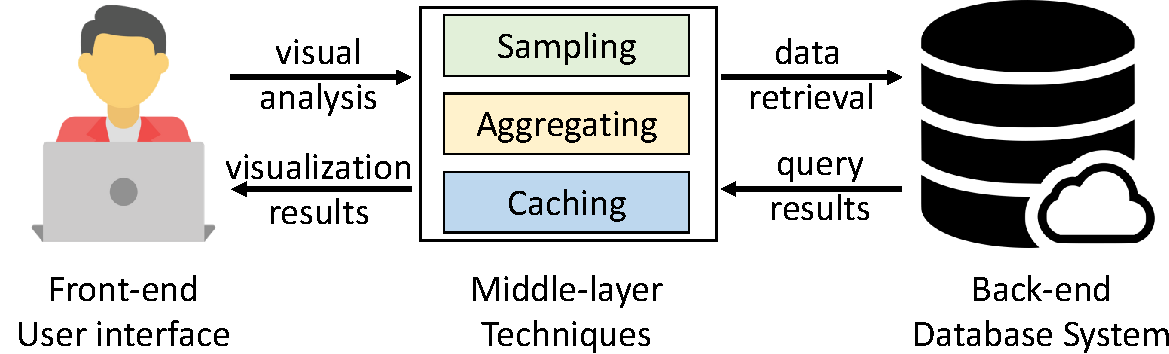
\includegraphics[width=0.36\textwidth]{pictures/framework/framework.pdf}
	\trim
	\caption{System architecture for interactive visualization.} \label{fig:sys_framework}
    \trim \trim
\end{figure}


\stitle{Aggregation-based techniques}
These works divide the {entire area} into basic units and visualize the aggregated information of the trajectories for each unit~\cite{wood2010visualisation,guo2009flow,von2015mobilitygraphs}. For more details on aggregation-based techniques, we refer the reader to~\cite{andrienko2008spatio,adrienko2010spatial}. Our problem and solutions are different from these works as we focus on visualizing the raw trajectories, instead of aggregated statistics.


\stitle{Sampling-based techniques} Sampling is widely used in both visualization and database communities ~\cite{battle2013dynamic,rapp2019void,chen2014visual,yu2020turbocharging,park2016visualization,qin2020making,DBLP:conf/sigmod/DingHCC016,DBLP:journals/pvldb/KimBPIMR15}. These works try to reduce the dataset to a subset with some special characteristics: such as blue noise property~\cite{rapp2019void}, multi-class property~\cite{chen2014visual} or maximize some user-defined quality~\cite{yu2020turbocharging}. The work most relevant to ours is~\cite{park2016visualization}, which is designed for scatter plots (a form of point-based visualization). It reduces the number of points in a plot while preserving the spatial distribution of the points in the original dataset. The techniques in~\cite{park2016visualization} cannot be applied to our trajectory visualization problem
as trajectory is more complex than individual scatter points (e.g., the order of GPS points is essential and the trajectories could have a large variance in length). Some works simplify a trajectory by sampling important points to reduce data size~\cite{zhang2018trajectory,2018arXiv180303550V} or alleviate visual clutter~\cite{borcan2012improving, 6851202}. These works are orthogonal to ours as we are sampling complete trajectories instead of points in a trajectory.



\stitle{Caching-based and other techniques}
Chan et al. propose ATLAS~\cite{chan2008maintaining}, which utilizes caching for efficient data communication between server and client.
ATLAS also exploits a powerful multi-core server to accelerate visual analysis tasks in both the middle-layer and back-end.
Piringer et al.~\cite{piringer2009multi} propose an architecture for interactive visual exploration,
which utilizes multi-core devices and avoids the common pitfalls of multi-threading to provide quick visual feedback.
Our work is orthogonal to these execution optimizations as we mainly focus on the algorithm perspective.

\sstitle{Novelties of our work} To the best of our knowledge, we are the first to formulate the quality optimal trajectory sampling problem to accelerate visualization on large scale datasets. We devise effective algorithms for this problem, which not only provide visual quality guarantee but also reduce the well-know visual clutter in trajectory visualization. Based on these algorithm, we design the $\avats$ framework with a tailored $\invQ$-tree index to produce high quality visualization for arbitrary target region with low latency.



\section{Problem Formulation}\label{sec:pro}
In this section,
we first formally define the \textit{quality optimal sampling problem} (\prob{}) for large-scale trajectory data visualization in Section~\ref{sec:def},
and then show that it is NP-hard to solve the problem exactly in Section~\ref{sec:hard}.

\begin{figure}
	\centering
	\small
	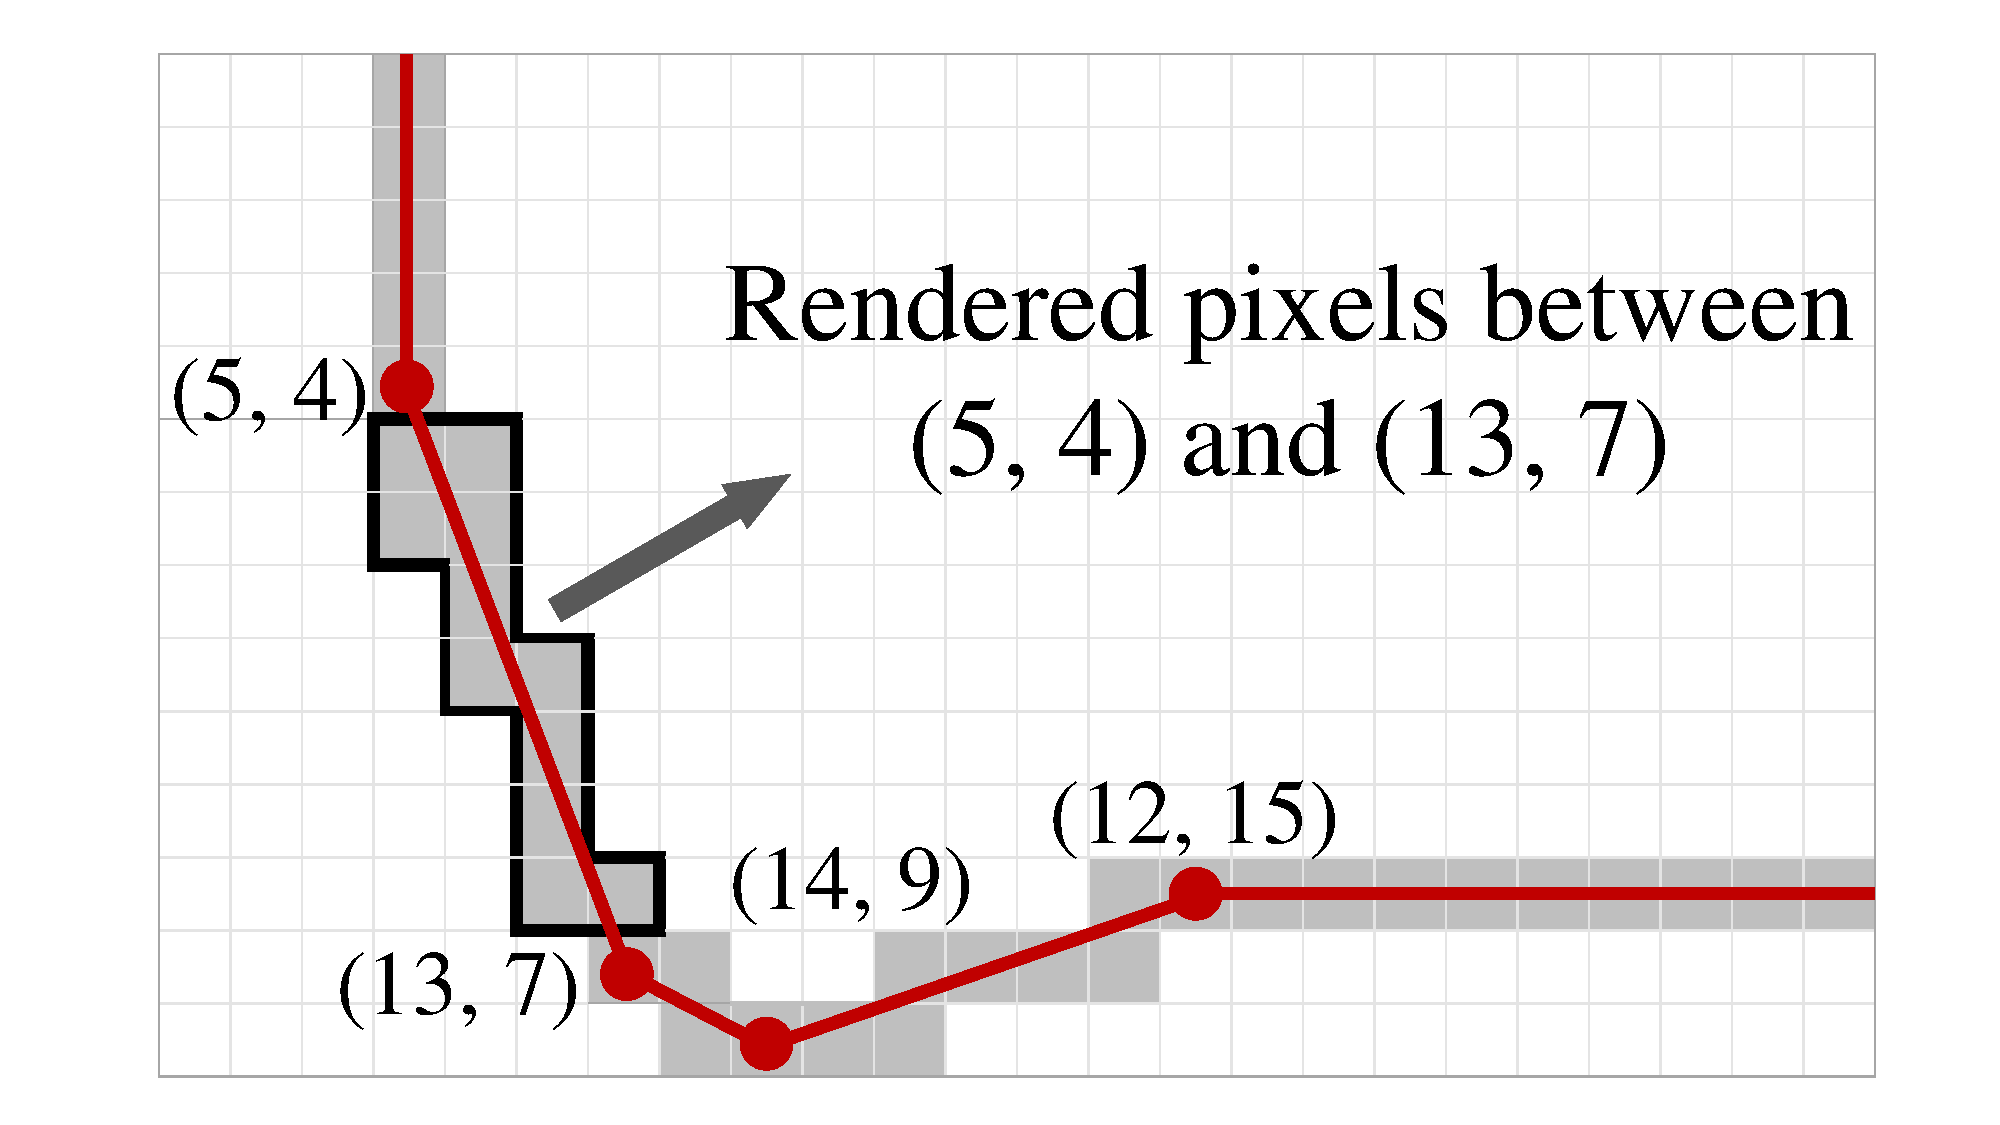
\includegraphics[width=0.45\columnwidth]{pictures/problemsolveing/RenderedPixels}  
    \trim
	\caption{Illustration of line-based trajectory visualization.} \label{fig:line}
    \trim \trim
\end{figure}


\subsection{Problem Definition}\label{sec:def}

We motivate our definition of the \textit{visualization quality function} by introducing how line-based trajectory visualization works.
As elaborated earlier, a trajectory contains a sequence of 2-dimensional locations.
Given an empty canvas (i.e., the screen of a displaying device) with pixels indexed by horizontal and vertical coordinates (i.e., $x$ and $y$), line-based trajectory visualization connects consecutive locations in each trajectory with polylines and marks the pixels passed by these polylines (with a color different from the background).
As shown in Figure~\ref{fig:line}(A), the result of line-based trajectory visualization can be regarded as a 2-dimensional array of boolean variables with 1 indicting that a pixel has been marked.
Alternatively, we can treat a visualization result as a set $\mathcal{S}=\{(x_i, y_i)\}_{i=1}^{n}$ that contains all marked pixels.
This observation leads to the following definition of visualization quality function
\begin{equation}\label{eqref:loss}
\QQ(\mathcal{S}, \mathcal{S}')=\frac{|\mathcal{S} \cap \mathcal{S}'|}{|\mathcal{S}|},
\end{equation}
in which $|.|$ measures the cardinality of a set, $\mathcal{S}$ is the visualization result of the entire trajectory dataset $\mathcal{T}$ while $ \mathcal{S}'$ is the visualization result of some trajectories sampled from $\mathcal{T}$.
As $\mathcal{S}'\subseteq \mathcal{S}$, $\QQ(\mathcal{S}, \mathcal{S}')$ essentially measures the ratio of the pixels in the ground-truth visualization $\mathcal{S}$ that are marked in the approximate visualization $\mathcal{S}'$.
%\footnote{For more general cases with $\mathcal{V}'\not\subset \mathcal{V}$, the quality function can be defined as $\mathsf{q}(\mathcal{V}, \mathcal{V}')\!=\!\frac{|\mathcal{V}-\mathcal{V}'|}{|\mathcal{V}|}$, in which set $\mathcal{V}^\star\!=\!\mathcal{V}-\mathcal{V}'$ contains all distinct elements between $\mathcal{V}$ and $\mathcal{V}'$.}.
This definition matches human visual perception and the approximate visualization $\mathcal{S}'$ will look similar to $\mathcal{S}$ if $\QQ(\mathcal{S}, \mathcal{S}')$ is large.
Sampling reduces the number of trajectories and location points to process, and thus shortens the visualization time.
With the quality function, we define the quality optimal sampling problem as follows.

\begin{problem}[Quality Optimal Sampling Problem, \prob{}]\label{prob:def}
Let the entire trajectory dataset be $\mathcal{T}$ and a sample set that contains some trajectories from $\mathcal{T}$ be $\mathcal{R}$.
Using $\VV(\mathcal{U})$ to denote the visualization result set derived from a trajectory set $\mathcal{U}$, with a sampling rate $\alpha$,
the quality optimal sampling problem finds a set $\mathcal{R}$ that satisfies
	\begin{equation}\label{eq:opp}
	\max_{\mathcal{R} \subseteq \mathcal{T}, |\mathcal{R}| = \lceil \alpha |\mathcal{T}| \rceil} \QQ(\VV(\mathcal{T}), \VV(\mathcal{R}))=\frac{|\VV(\mathcal{T}) \cap \VV(\mathcal{R})|}{|\VV(\mathcal{T})|}.
	\end{equation}
\end{problem}
Note that we are sampling \textit{complete trajectories} instead of \textit{individual locations} in \prob{} such that the lines and orientations in the trajectories are persevered.

Intuitively, given a visualization quality threshold $\tau$, the \prob{} problem can be transformed to find the sampled trajectory set $\mathcal{R}$ with the smallest $\alpha$,
under which provides the quality requirement holds, i.e, $\QQ(\VV(\mathcal{T}), \VV(\mathcal{R})) \!\ge\! \tau$.




\subsection{Hardness Analysis}\label{sec:hard}
We use $t_i\! \in \! \mathcal{T}$ to denote a trajectory in the dataset.
According to the working mechanism of line-based trajectory visualization, $t_i$ corresponds to a set of marked pixels on the canvas in the ground-truth visualization $\VV(\mathcal{T})$ and we also use $t_i$ to denote this set of pixels.
Thus, we have $\VV(\mathcal{T}) = \cup_{t_i \in \mathcal{T}} t_i$ and $\VV(\mathcal{R}) = \cup_{t_i \in \mathcal{R}} t_i$.
We can transform Problem~\ref{prob:def} as follows:

\begin{align}\label{eqn:obj2}
& \max_{\oR \subseteq \D, |\oR| = \lceil \alpha |\mathcal{T}| \rceil}  \frac{|\VV(\mathcal{T}) \cap \VV(\mathcal{R})|}{|\VV(\mathcal{T})|} \\ \nonumber
& \Leftrightarrow \max_{\oR \subseteq \D, |\oR| = \lceil \alpha |\mathcal{T}| \rceil}   |\VV(\oR)|   %\\ \nonumber
 \Leftrightarrow \max_{\oR \subseteq \D, |\oR| = \lceil \alpha |\mathcal{T}| \rceil} | \cup_{t_i \in \oR} t_i |.
\end{align}

%\begin{align}\label{eqn:obj5} \nonumber
%	\min_{\oR \subseteq \D, |\oR| = \alpha |\D|}  \frac{|\V(\D) - \V(\oR)|}{|\V(\D)|}  & \Leftrightarrow \min_{\oR \subseteq \D, |\oR| = \alpha |\D|}   - |\V(\oR)| \\ \nonumber
%	\Leftrightarrow \max_{\oR \subseteq \D, |\oR| = \alpha |\D|}  |\V(\oR)| &  \Leftrightarrow \max_{\oR \subseteq \D, |\oR| = \alpha |\D|} | \cup_{t_i \in \oR} t_i |
%\end{align}

The transformations use the fact that $\VV(\mathcal{R}) \!\subseteq \! \VV(\mathcal{T})$ as $\mathcal{R}\! \subseteq \! \mathcal{T}$, and the ground-truth marked point set $\VV(\mathcal{T})$ has constant cardinality.
The last line shows that \prob{} is equivalent to the famous set cover maximization problem\footnote{\url{https://en.wikipedia.org/wiki/Maximum_coverage_problem}}.
Specifically, given an integer $k$, and a collection of sets $\D = \{t_1, t_2, \cdots, t_n \}$,
set cover maximization finds a subset $\oR \subset \D$ such that $|\oR| = k$ and the number of covered elements $|\cup_{t_i \in \oR} t_i|$ is maximized.
The set cover maximization problem is well-known to be NP-hard~\cite{algorithms}.
For sampling-based methods, the visualization quality is determined by the sample set $\mathcal{R}$,
and thus we use $\QQ(\mathcal{R})$ to denote $\QQ(\VV(\mathcal{T}), \VV(\mathcal{R}))$ for conciseness.




%It is equivalent to select sized-$k$ trajectory set $\oR$ from $\D$ which $\cup_{\oR_i \in \oR} \oR_i$ is maximized.
%It is a NP-hard problem as we proved in Lemma~\ref{lem:np}.

%\begin{lemma}[NP hard]~\label{lem:np}
%Given a trajectory dataset $\D$ and an integer $k$,
%The sampling-based trajectory visualization problem (see Problem~\ref{prob:def}) is NP-hard.
%\end{lemma}

%We omit the proof of Lemma~\ref{lem:np} as it is a typical set cover maximization problem\footnote{\url{https://en.wikipedia.org/wiki/Maximum_coverage_problem}}, which is a well-known NP-hard problem in literature.

%------------comments by Bo-------------------
%As we analyzed in Section~\ref{sec:intro}, the large-scale (e.g., hundreds of millions GPS points) line-based trajectory visualization problem is very challenging due to the large data size and limited rendering capability of graphics devices.
%To make matters worse, the visualization result of large-scale trajectory dataset suffers visual clutter seriously.
%In this work, we focus on how to visualize large-scale trajectory dataset efficiently and effectively.
%In particular, our objective is to devise a visual quality guaranteed sampling method for large trajectory data visualization.
%The major challenges to achieve this goal are:
%(i) how to define visual quality theoretically? (ii) how to guarantee the visual quality of the sampling-based visualization result?


\section{Solutions for \prob{}}\label{sec:sol}
In this section,  we first present the $\vats$ algorithm as a solution to \prob{} and propose techniques to boost its efficiency.
Then we improve $\vats$ with an advanced algorithm $\vatss$ by considering trajectory data distribution and human perception capability.


\subsection{Visual Quality Guaranteed Sampling $\vats$}\label{sec:greedy}
%Due to the hardness of Problem~\ref{prob:def}, the straight-forward solution is uniform random sampling $\rand$.
%This solution randomly selects $k$ trajectories from the dataset $\D$ and stores them in the result set $\oR$. The selected trajectories in $\oR$ are rendered as the visualization result.
%Obviously, uniform random sampling $\rand$ does not provide any guarantee on the visual quality of the sampled set.



\begin{algorithm}
    \caption{$\vats(\D, k=\lceil \alpha |\mathcal{T}| \rceil$)} \label{alg:greedy}
    \begin{algorithmic}[1]
    \State Initialize the result set $\oR \leftarrow \emptyset$
    \While{$|\oR| < k$}
        \State $\mathsf{tmp} \leftarrow \arg\max_{t_i \in \D} |t_i \cup \VV(\oR)|$ \label{line:max}
        \State $\oR \leftarrow \oR \cup \{ \mathsf{tmp} \}$
    \EndWhile
    \State Return $\oR$
    \end{algorithmic}
\end{algorithm}

Our visual quality guaranteed sampling method ($\vats$) is presented in Algorithm~\ref{alg:greedy},
which takes the trajectory dataset $\D$ and a sampling rate $\alpha$ as input (i.e., $k=\lceil \alpha |\mathcal{T}| \rceil$).
$\vats$ employs a greedy paradigm and finds the trajectory $\mathsf{tmp}$ in $\D$ that maximizes $| \mathsf{tmp} \cup \VV(\oR)|$ at each iteration, as shown in Line~\ref{line:max} of Algorithm~\ref{alg:greedy}.
It terminates after $k=\lceil \alpha |\mathcal{T}| \rceil$ iterations and returns $\oR$ as the result set.
As the visualization quality $\QQ(\mathcal{R})$ can be computed after each iteration in Algorithm~\ref{alg:greedy} with pre-computed ground-truth $\VV(\mathcal{T})$,
we can also terminate the algorithm when $\VV(\mathcal{R})\ge \tau$, in which $\tau$ is the quality threshold. Algorithm~\ref{alg:greedy} provides provable visual quality guarantee for the result set $\oR$, as stated in Theorem~\ref{the:ratio}.

\begin{theorem}~\label{the:ratio} Given a sample rate $\alpha$, and let the optimal solution to \prob{} defined in Equation~\eqref{eq:opp} be $\mathcal{R}^{\star}$ and the solution provided by Algorithm~\ref{alg:greedy} be $\mathcal{R}$, we have $\QQ(\mathcal{R})\ge 0.632*\QQ(\mathcal{R}^{\star})$.
\end{theorem}

Theorem~\ref{the:ratio} follows directly from the submodularity of the visualization quality function $\QQ(\mathcal{R})$,
and it is well known that greedy solution provides a $0.632$ approximation of the optimal solution for a submodular function~\cite{fujishige2005submodular}.
As $\QQ(\mathcal{R})$ is a linear scaling of $|\VV(\oR)|$ as shown in Equation~\eqref{eqn:obj2}, we prove  $|\VV(\oR)|$ is submodular as follows.

\begin{lemma}[Submodularity]\label{lem:submodular}
Define the contribution value of a trajectory $t$ to a sample set $\oR$ as $\Delta(\oR, t) = |\VV(\oR \cup t)| - |\VV(\oR)|$.
Given a trajectory $t$ and two sample sets $\oR,\oR^{'}$, if $\oR \subset \oR^{'}$, then $ \Delta(\oR, t) \geq \Delta(\oR^{'}, t)$.
\end{lemma}

\begin{proof}
The contribution value of trajectory $t$ w.r.t. a given result set $\oR$ (i.e., $\Delta(\oR, t) = |\VV(\oR \cup t)| - |\VV(\oR)|$) is the number of pixels covered by $t$ but not the trajectory set $\oR$,
which can be expressed as $|\VV(t)| - |\VV(\oR) \cap \VV(t))|$.
We have $\VV(t) \cap \VV(\oR) \subseteq \VV(t) \cap \VV(\oR^{'}) $ because $\oR^{'}$ is a superset of $\oR$, which implies $|\VV(t)| - |\VV(\oR) \cap \VV(t))| \geq |\VV(t)| - |\VV(\oR^{'})\cap \VV(t))|$.
Thus, it holds that $\Delta(\oR, t) = |\VV(\oR \cup t)| - |\VV(\oR)| \geq |\VV(\oR^{'} \cup t)| - |\VV(\oR^{'})|= \Delta(\oR^{'}, t)$.
\end{proof}


%\begin{proof}
%The optimal solution of Problem~\ref{prob:def} covers $f(\mathcal{R}^{\star})$ pixels in $k$ iterations.
%Let $a_i$ be the number of newly covered pixels at the $i$-th iteration, $b_i$ is the total number of covered pixels up to the $i$-th iteration (i.e., $b_i = \sum_{j=1}^{i}a_i$),
%and $c_i$ be the uncovered pixels after $i$-th iteration (i.e., $c_i = f(\mathcal{R}^{\star})-b_i$).
%According to greedy paradigm, we can conclude the number of newly covered pixels at the $(i+1)$-th iteration is always greater than or equal to $\frac{1}{k}$ of the number of uncovered pixels after the $i$-th iteration, i.e., $a_{i+1} \geq \frac{c_i}{k}$.
%We prove Theorem~\ref{the:ratio} by proving $c_{i+1} \leq (1-1/k)^{i+1} \cdot f(\mathcal{R}^{\star})$.
%It holds $c_1 \leq (1-1/k) \cdot f(\mathcal{R}^{\star})$ as follows.
%\begin{align} \nonumber
%& a_1 \geq c_0 \cdot 1/k = 1/k \cdot f(\mathcal{R}^{\star}) \text{~~~as we concluded~~~} a_{i+1} \geq \frac{c_i}{k}\\ \nonumber
% \Leftrightarrow  & b_1 \geq 1/k \cdot f(\mathcal{R}^{\star})  \Leftrightarrow  -b_1 \leq - 1/k \cdot f(\mathcal{R}^{\star})  \text{~~~as~~~} a_1 = b_1\\ \nonumber
% \Leftrightarrow & f(\mathcal{R}^{\star}) - b_ 1 \leq f(\mathcal{R}^{\star}) - 1/k \cdot f(\mathcal{R}^{\star})  \Leftrightarrow  c_1 \leq (1-1/k) \cdot f(\mathcal{R}^{\star})
%\end{align}
%For inductive hypothesis assume $c_{i} \leq (1-1/k)^i \cdot f(\mathcal{R}^{\star})$. Thus,
%\begin{align} \nonumber
%& c_{i+1} = c_i - a_{i+1} \leq c_i - c_i/k = (1-1/k) \cdot c_i =  (1-1/k)^{i+1} \cdot f(\mathcal{R}^{\star})
%\end{align}
%
%Hence, it holds $c_k \leq (1-1/k)^{k} \cdot f(\mathcal{R}^{\star})$.
%It is equivalent to $b_k = f(\mathcal{R}) \geq (1 - (1-1/k)^{k}) \cdot f(\mathcal{R}^{\star}) \geq (1-1/e) \cdot f(\mathcal{R}^{\star}) \approx 0.632 \cdot f(\mathcal{R}^{\star})$.
%\end{proof}


Although Algorithm~\ref{alg:greedy} provides quality guarantee for the result set $\oR$, it has a high time complexity, which we show as follows.

%With the above theoretical analysis, Algorithm~\ref{alg:greedy} offers a visual quality-guaranteed sampling algorithm for the large-scale trajectory data visualization problem.
%However, as the time complexity analyzed in Lemma~\ref{lem:cost}, it is not scalable to large-scale trajectory datasets (e.g., millions of trajectories).


\begin{lemma}[Time Complexity]~\label{lem:cost}
For a trajectory dataset $\D$ and an integer $k=\lceil \alpha |\mathcal{T}| \rceil$, the time complexity of Algorithm~\ref{alg:greedy} is $O(\alpha \cdot m \cdot |\D|^2)$,
where $m$ is the maximum length for the trajectories in $\D$.
\end{lemma}


\begin{proof}
In each iteration, Algorithm~\ref{alg:greedy} computes the trajectory with the largest number of uncovered pixels in dataset $\D$.
It take $O(m)$ cost to compute the number of uncovered pixels for each trajectory in $\D$.
Algorithm~\ref{alg:greedy} runs for $k=\lceil \alpha |\mathcal{T}| \rceil$ iterations.
Hence, the total cost is $O(k \cdot m \cdot |\D|)=O(\alpha \cdot m \cdot |\D|^2)$.
\end{proof}
The high complexity of Algorithm~\ref{alg:greedy} hurts its scalability for large-scale trajectory datasets.
% even though sampling is conducted in the offline index building phase for CheetahTraj.
For example, the \pt{} dataset contains 2.39 millions taxi trajectories, Algorithm~\ref{alg:greedy} takes 413.6 seconds to obtain the result set $\oR$ with sampling rate $0.1\%$.

%and the longest trajectory has 3,490 GPS points
%Obviously, the running time is too long for interactive trajectory exploration.

\begin{figure}
	\centering
	\small
	\begin{tabular}{cc}
		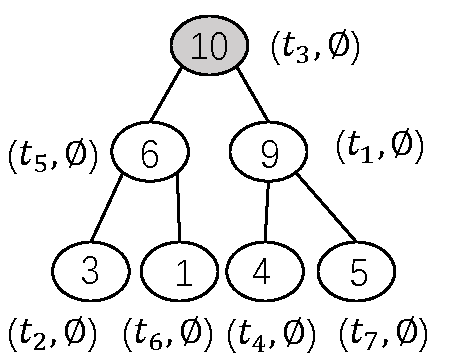
\includegraphics[width=0.42\columnwidth]{pictures/1st}
		&
		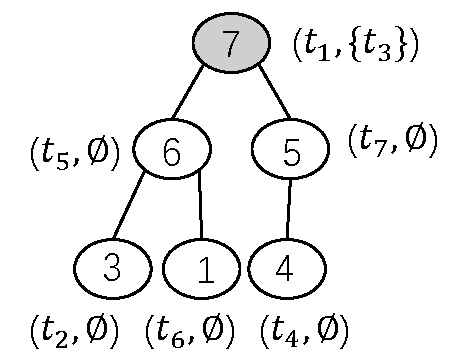
\includegraphics[width=0.42\columnwidth]{pictures/2nd}
		\\
		(A) 1st iteration
		&
		(B) 2nd iteration
	\end{tabular}
    \trim
    \vspace{-2mm}
	\caption{Heap-based lazy computation.} \label{fig:heap} %via the submodularity in Lemma~\ref{lem:submodular}
    \trim \trim
\end{figure}


\stitle{Heap-based lazy Computation}
Algorithm~\ref{alg:greedy} essentially adds the trajectory that maximizes $\Delta(\oR, t) = |\VV(\oR \cup t)| - |\VV(\oR)|$ to $\oR$ in each iteration.
Lemma~\ref{lem:submodular} shows that the contribution of a trajectory (i.e., $\Delta(\oR, t)$) cannot increase when Algorithm~\ref{alg:greedy} runs for more iterations because $ \Delta(\oR^{'}, t) \le \Delta(\oR, t) $ for  $\oR \subset \oR^{'}$.
For example, the contribution of $t_1$ is $9$ at the first iteration (i.e., $\oR = \emptyset$), see Figure~\ref{fig:heap}(a).
Its contribution turns $7$ when $\oR = \{ t_3 \}$ at the second iteration, as shown in Figure~\ref{fig:heap}(b).
Based on this property, we can use  $\Delta(\oR, t)$ calculated in the previous iterations to prune it from contribution computation.
Specifically, if we have $\Delta(\oR, t) \le \Delta(\oR^{'}, t')$, in which $\oR$ and $\oR^{'}$ are a previous and the current sample set, respectively,
we know that $t$ can not be added to the sample set in the current iteration as $\Delta(\oR^{'}, t)\le \Delta(\oR^{'}, t')$ and $t'$ is a better choice.
As shown in Figure~\ref{fig:heap}(b), even if we do not know the exact value of $\Delta(\oR'=\{t_3\}, t_7)$,
we can conclude that $t_7$ will not be added to the sample set in the second iteration as $\Delta(\oR = \emptyset, t_7) = 5 < \Delta(\oR'=\{t_3\}, t_1) = 7$.


To implement this idea, we maintain a max-heap for the number of uncovered pixels in each trajectory and update the contribution of a trajectory only when necessary, i.e., computing in a lazy manner. Consider a tiny example with 7 trajectories, i.e., $t_1$ to $t_7$.
Figure~\ref{fig:heap}(a) shows the initial max-heap and the contributions of trajectories $t_1$ to $t_7$ w.r.t. result set $\oR = \emptyset$.
At the first iteration, the root node of the max-heap, $t_3$ in Figure~\ref{fig:heap}(A), is selected.
At the second iteration, the number of uncovered pixels of the new root node $t_1$ is updated to 7 w.r.t. result set $\oR = \{ t_3 \}$ (the gray node in Figure~\ref{fig:heap}(B)).
Then $t_1$ is selected at the second iteration without computing the contributions of other trajectories w.r.t. $\oR = \{ t_3 \}$.
This is because the contributions of these trajectories are less than 7 when $\oR = \emptyset$,
according to Lemma~\ref{lem:submodular}, their contributions must be smaller than $7$ when $\oR = \{ t_3 \}$.
The efficiency of Algorithm~\ref{alg:greedy} improves significantly with heap-based lazy computation.
Recall that Algorithm~\ref{alg:greedy} takes 413.6 seconds with $\alpha=0.1\%$ on \pt{} while our performance-optimized $\vats$ needs only 1.2 seconds.

%In summary, the number of uncovered pixels in each trajectory will only be computed with the latest result set $\oR$ when it is necessary in the lazy computing manner,
%e.g., only $t_1$ will be updated at the 2nd iteration in Figure~\ref{fig:heap}.
%It reduces many unnecessary computations through the lazy updating manner, e.g., all white nodes did not update at the 2nd iteration in the above example.

%We then analyze the time complexity of Algorithm~\ref{alg:greedy} with lazy computing manner in Theorem~\ref{lem:lazy}.
%
%\begin{lemma}[Optimized Time Complexity]~\label{lem:lazy}
%Given trajectory dataset $\D$ and an integer $k= \alpha |\D|$, the time complexity of Algorithm~\ref{alg:greedy} with lazy computing manner is $O(\alpha \cdot m \cdot x |\D| \log |\D|)$, where $x$ is the number of contribution computations among all $k$ iterations and $x \ll |\D|$.
%\end{lemma}
%
%\begin{proof}
%It first takes $O(|\D|)$ time to construct the max-heap~\cite{cormen2009introduction}.
%It incurs $O( m \cdot x \log |\D|)$ cost to select the trajectory with maximum uncovered pixels at each iteration ($k$ iterations in total).
%Hence, the overall cost is $O(|\D| + k \cdot m \cdot t \log |\D|)$.
%\end{proof}

\subsection{Advanced Approach $\vatss$}\label{subsec:VQGS+}

\begin{figure*}
   \begin{minipage}{0.65\textwidth}
     \centering
     \begin{tabular}{ccc}
     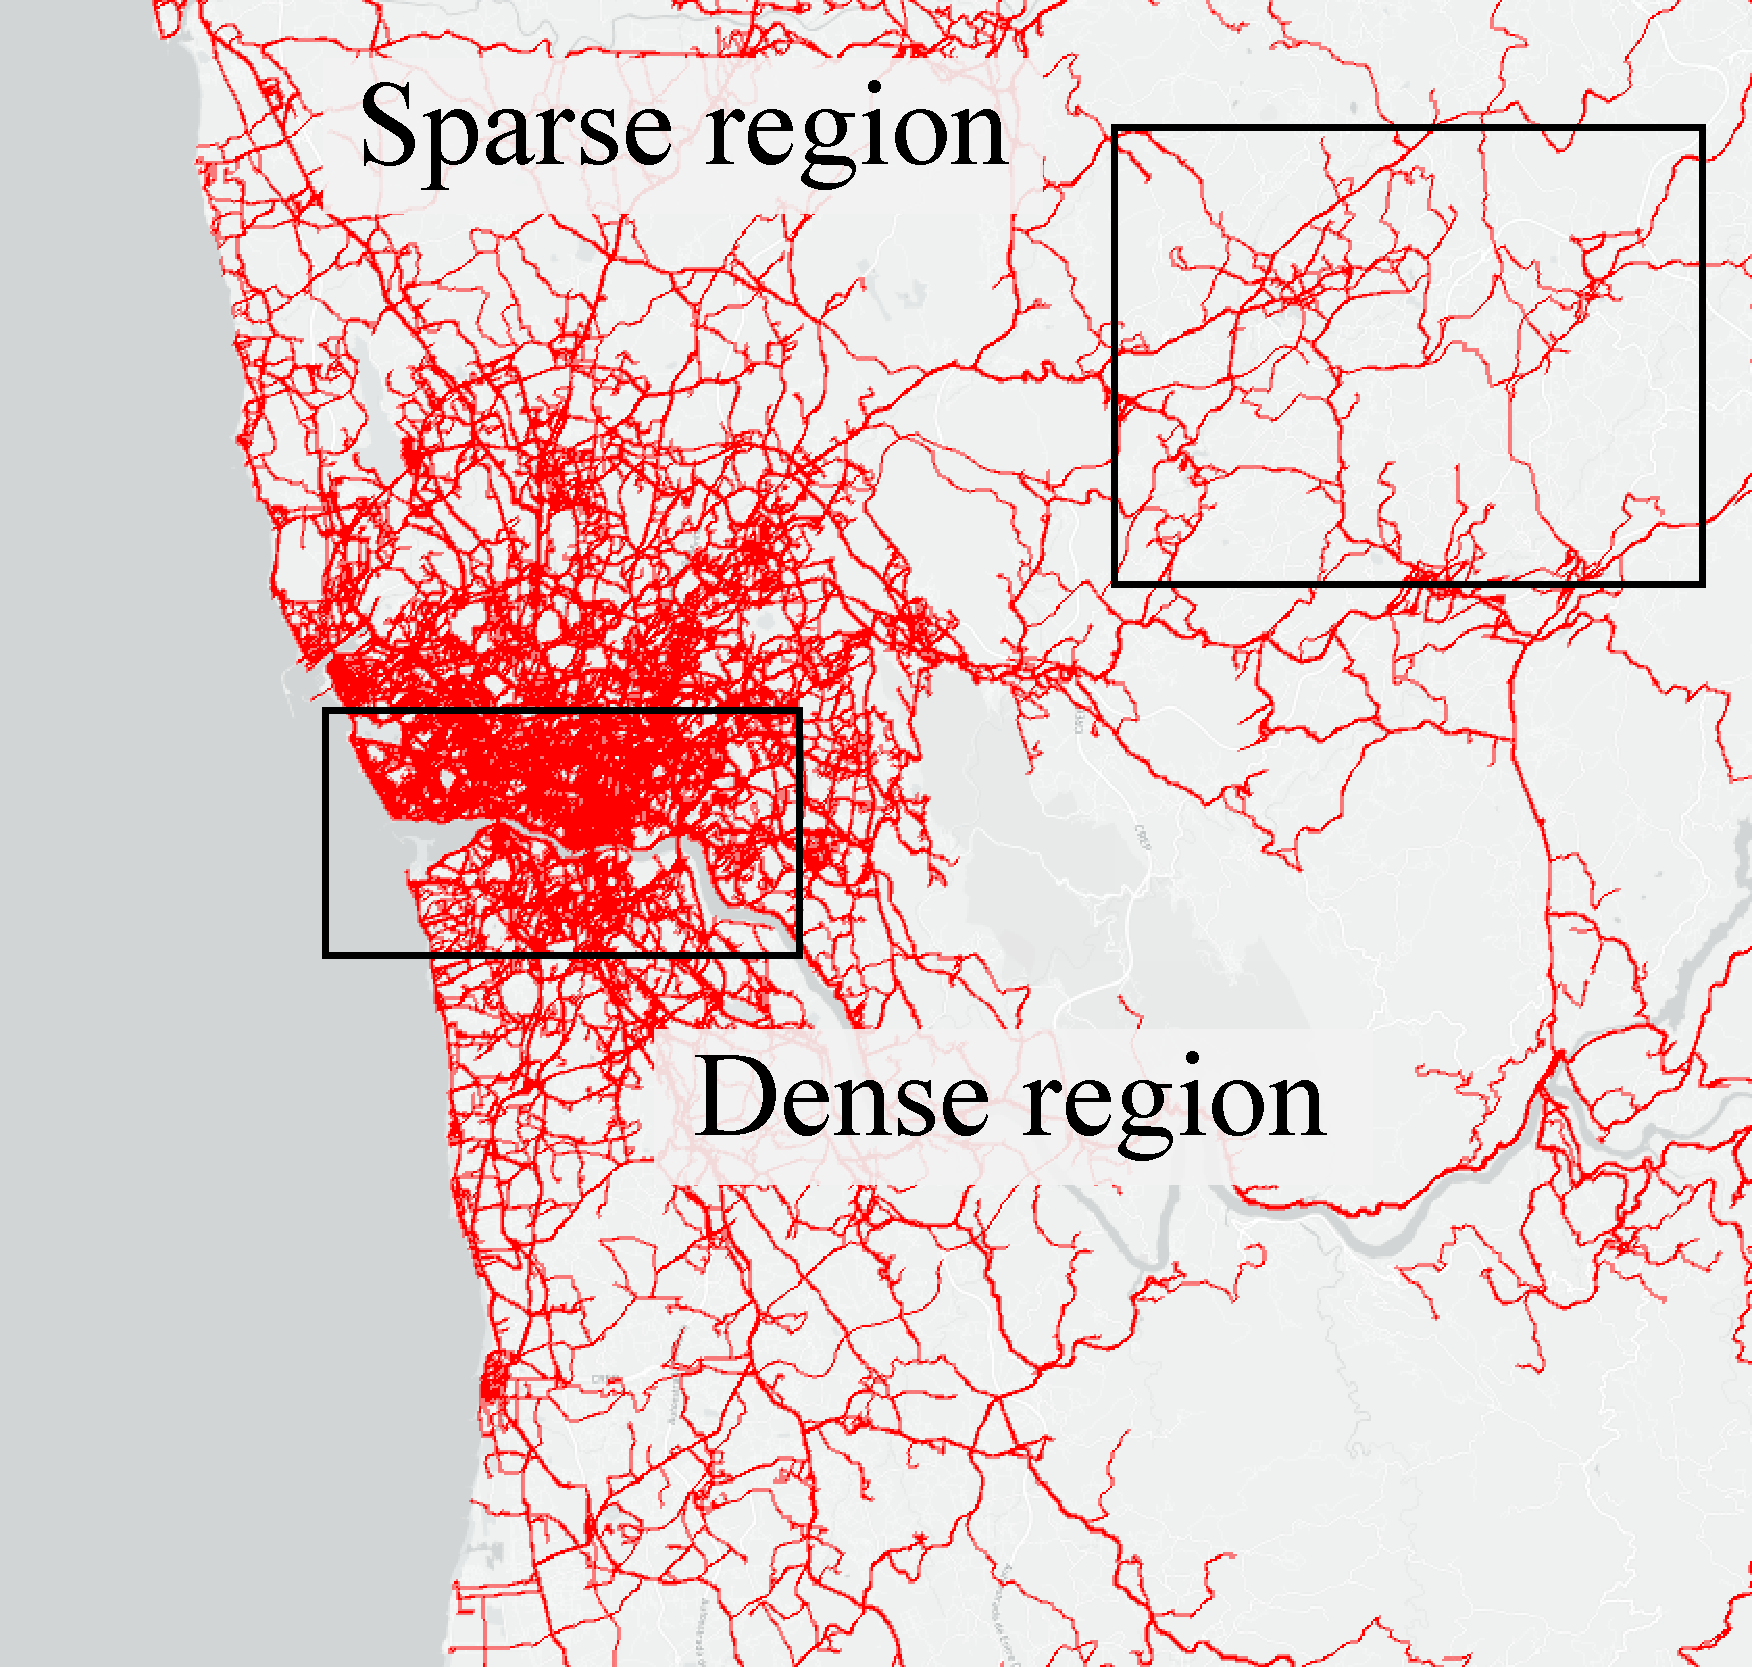
\includegraphics[width=0.22\linewidth]{pictures/motivation_VQGS}
     &
     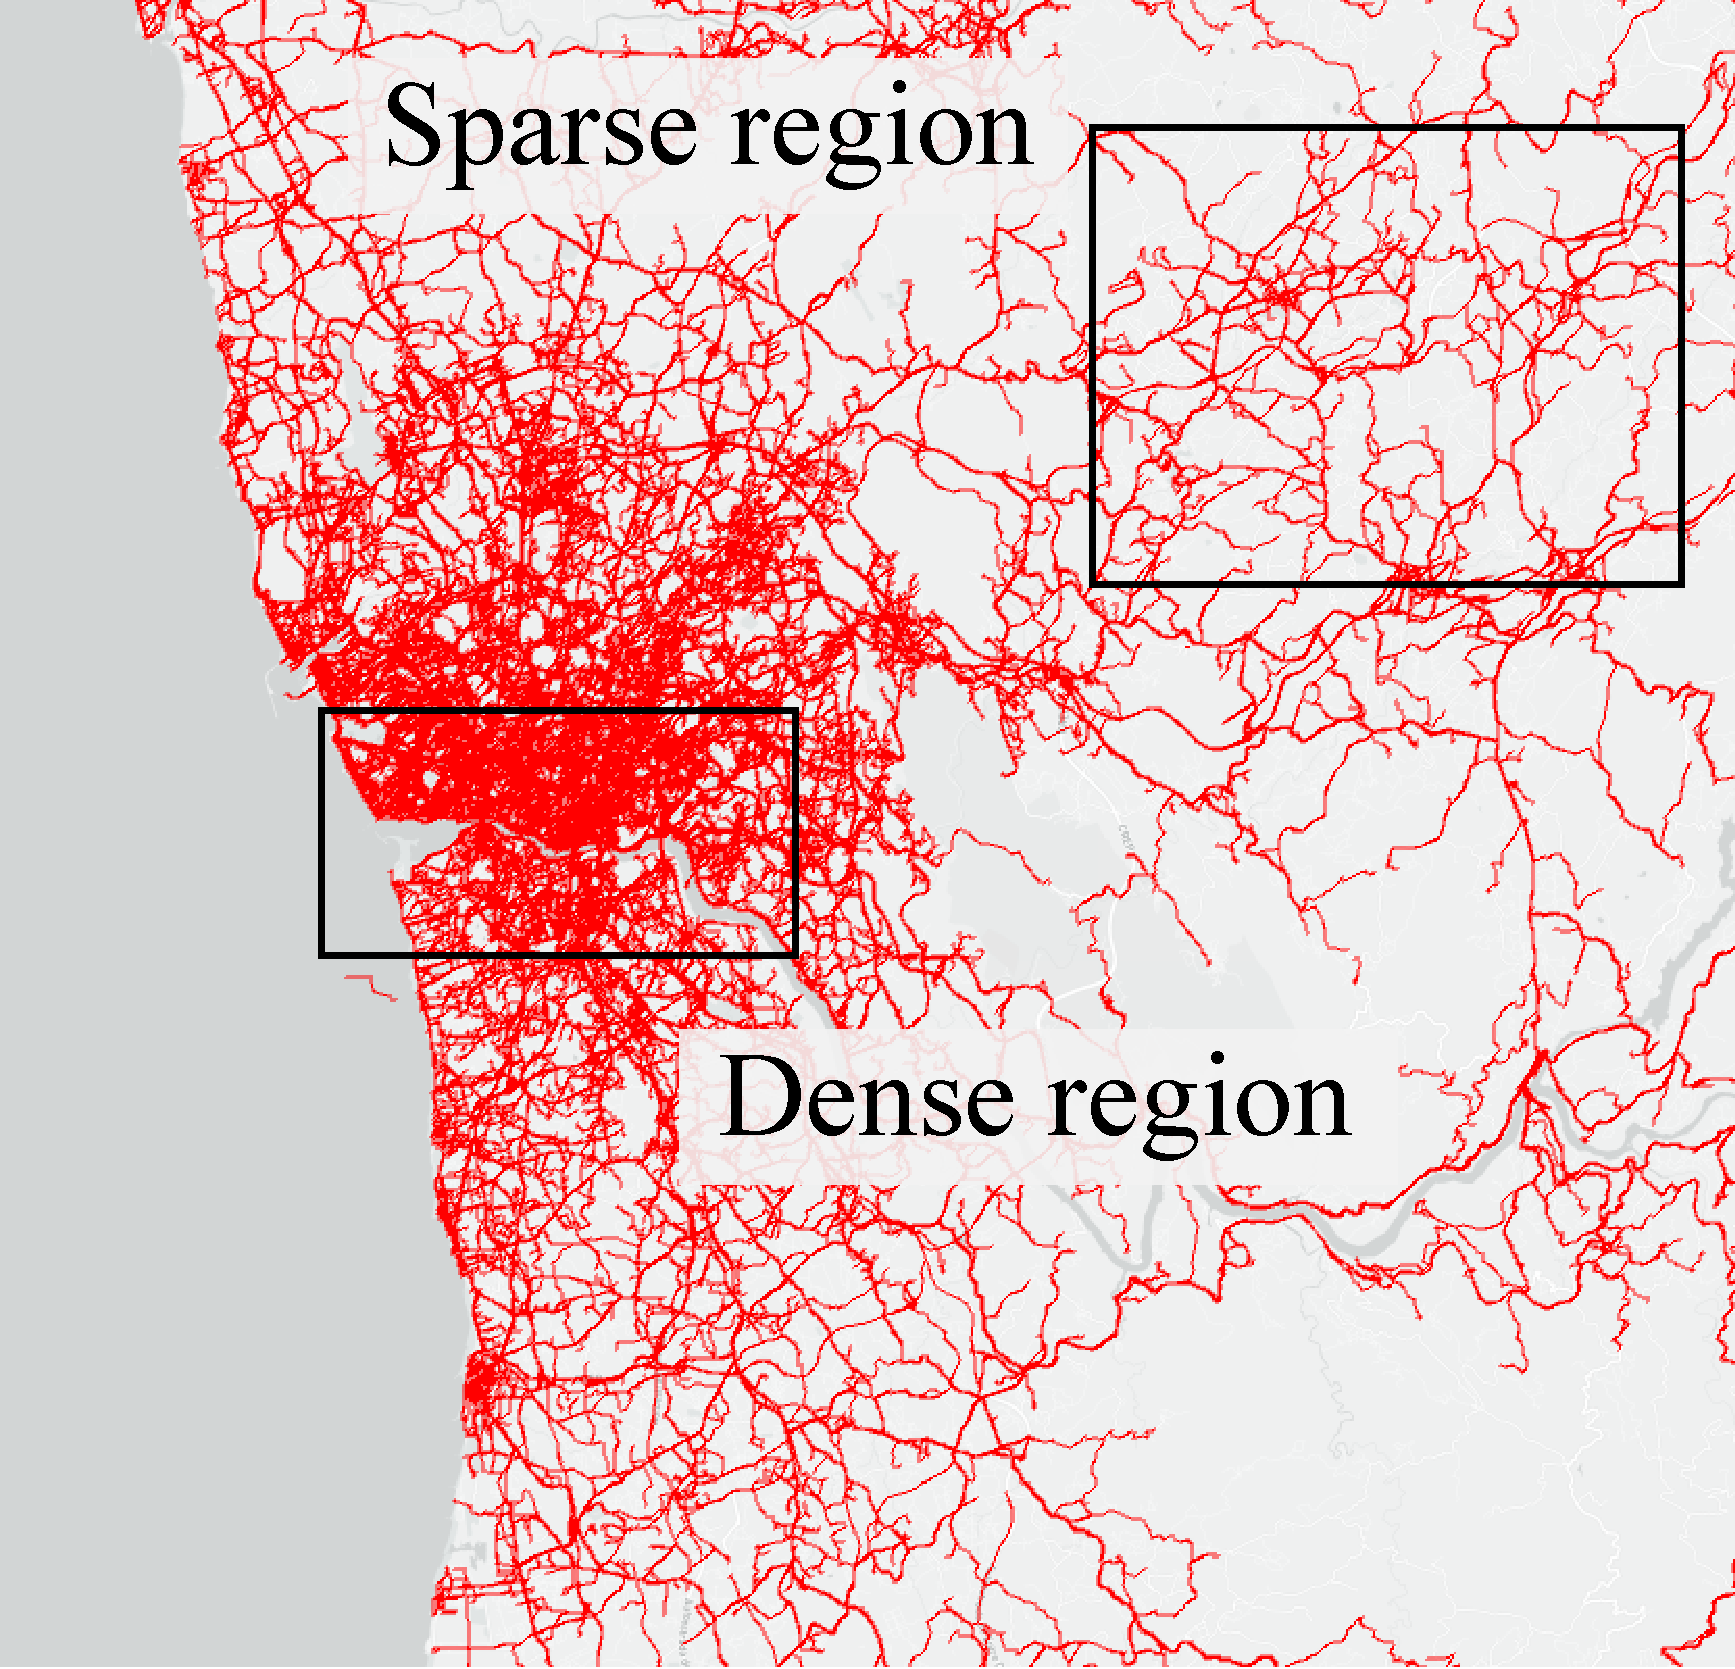
\includegraphics[width=0.22\linewidth]{pictures/motivation_VQGS+d64}
     &
     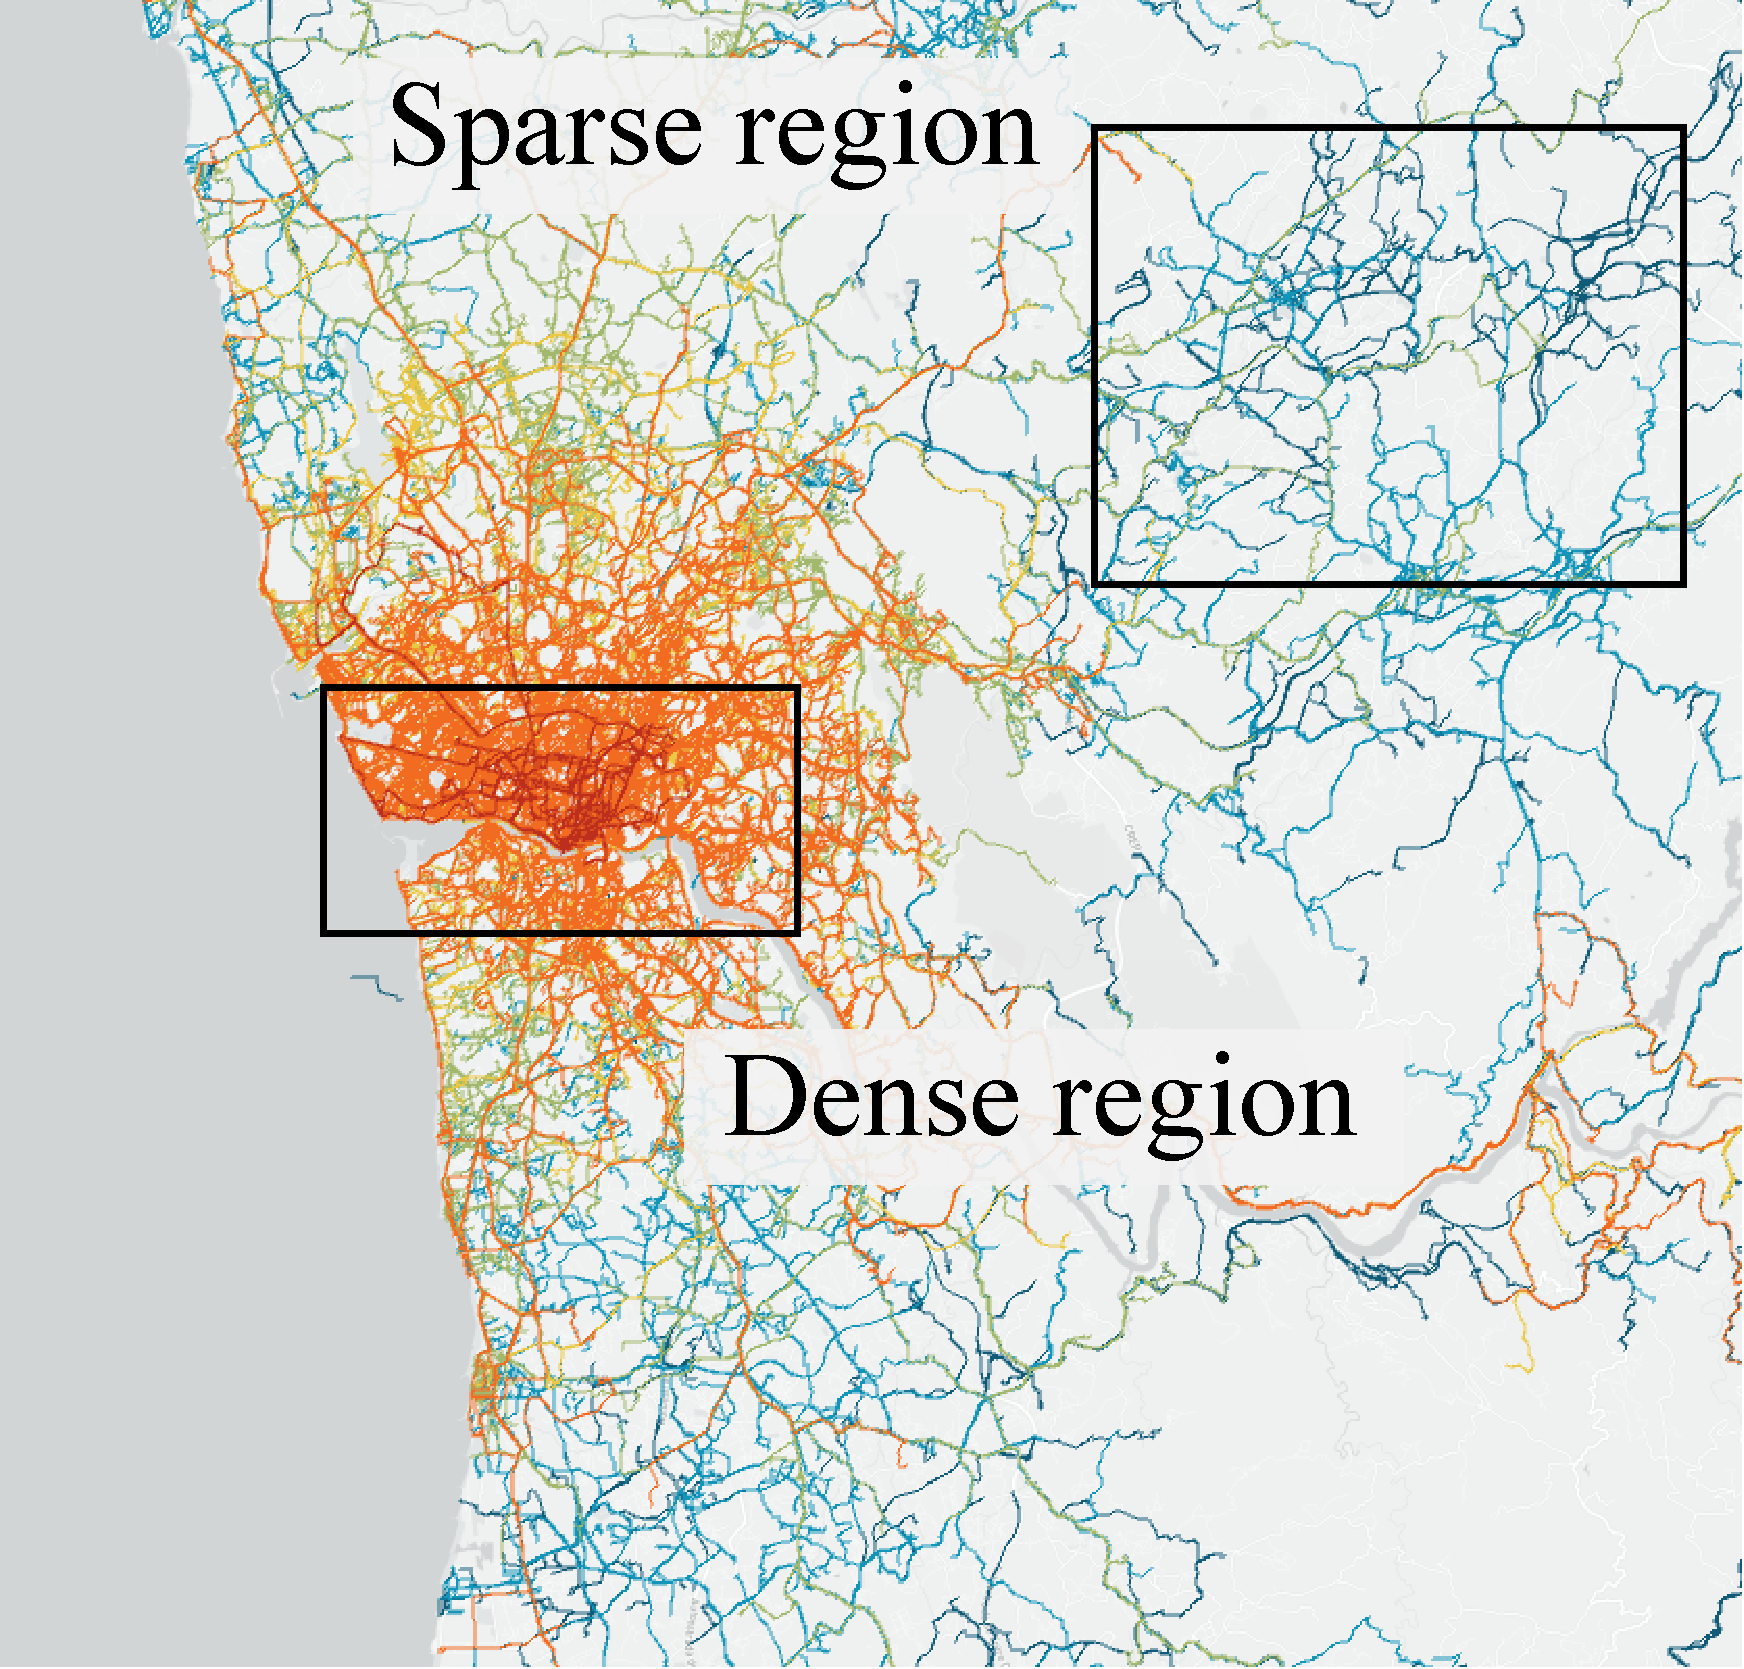
\includegraphics[width=0.22\linewidth]{pictures/motivation_VQGS+d64CE}
     \\
     (A) $\vats$
     &
     (B) $\vatss$
     &
     (C) $\vatssce$
     \end{tabular}
     \trim
     \caption{\prob{} solution $\vatss$ on \pt{} ($\alpha = 0.5\%, \delta = 64$)}\label{fig:delta}.
   \end{minipage}\hfill
   \begin{minipage}{0.35\textwidth}
     \centering
     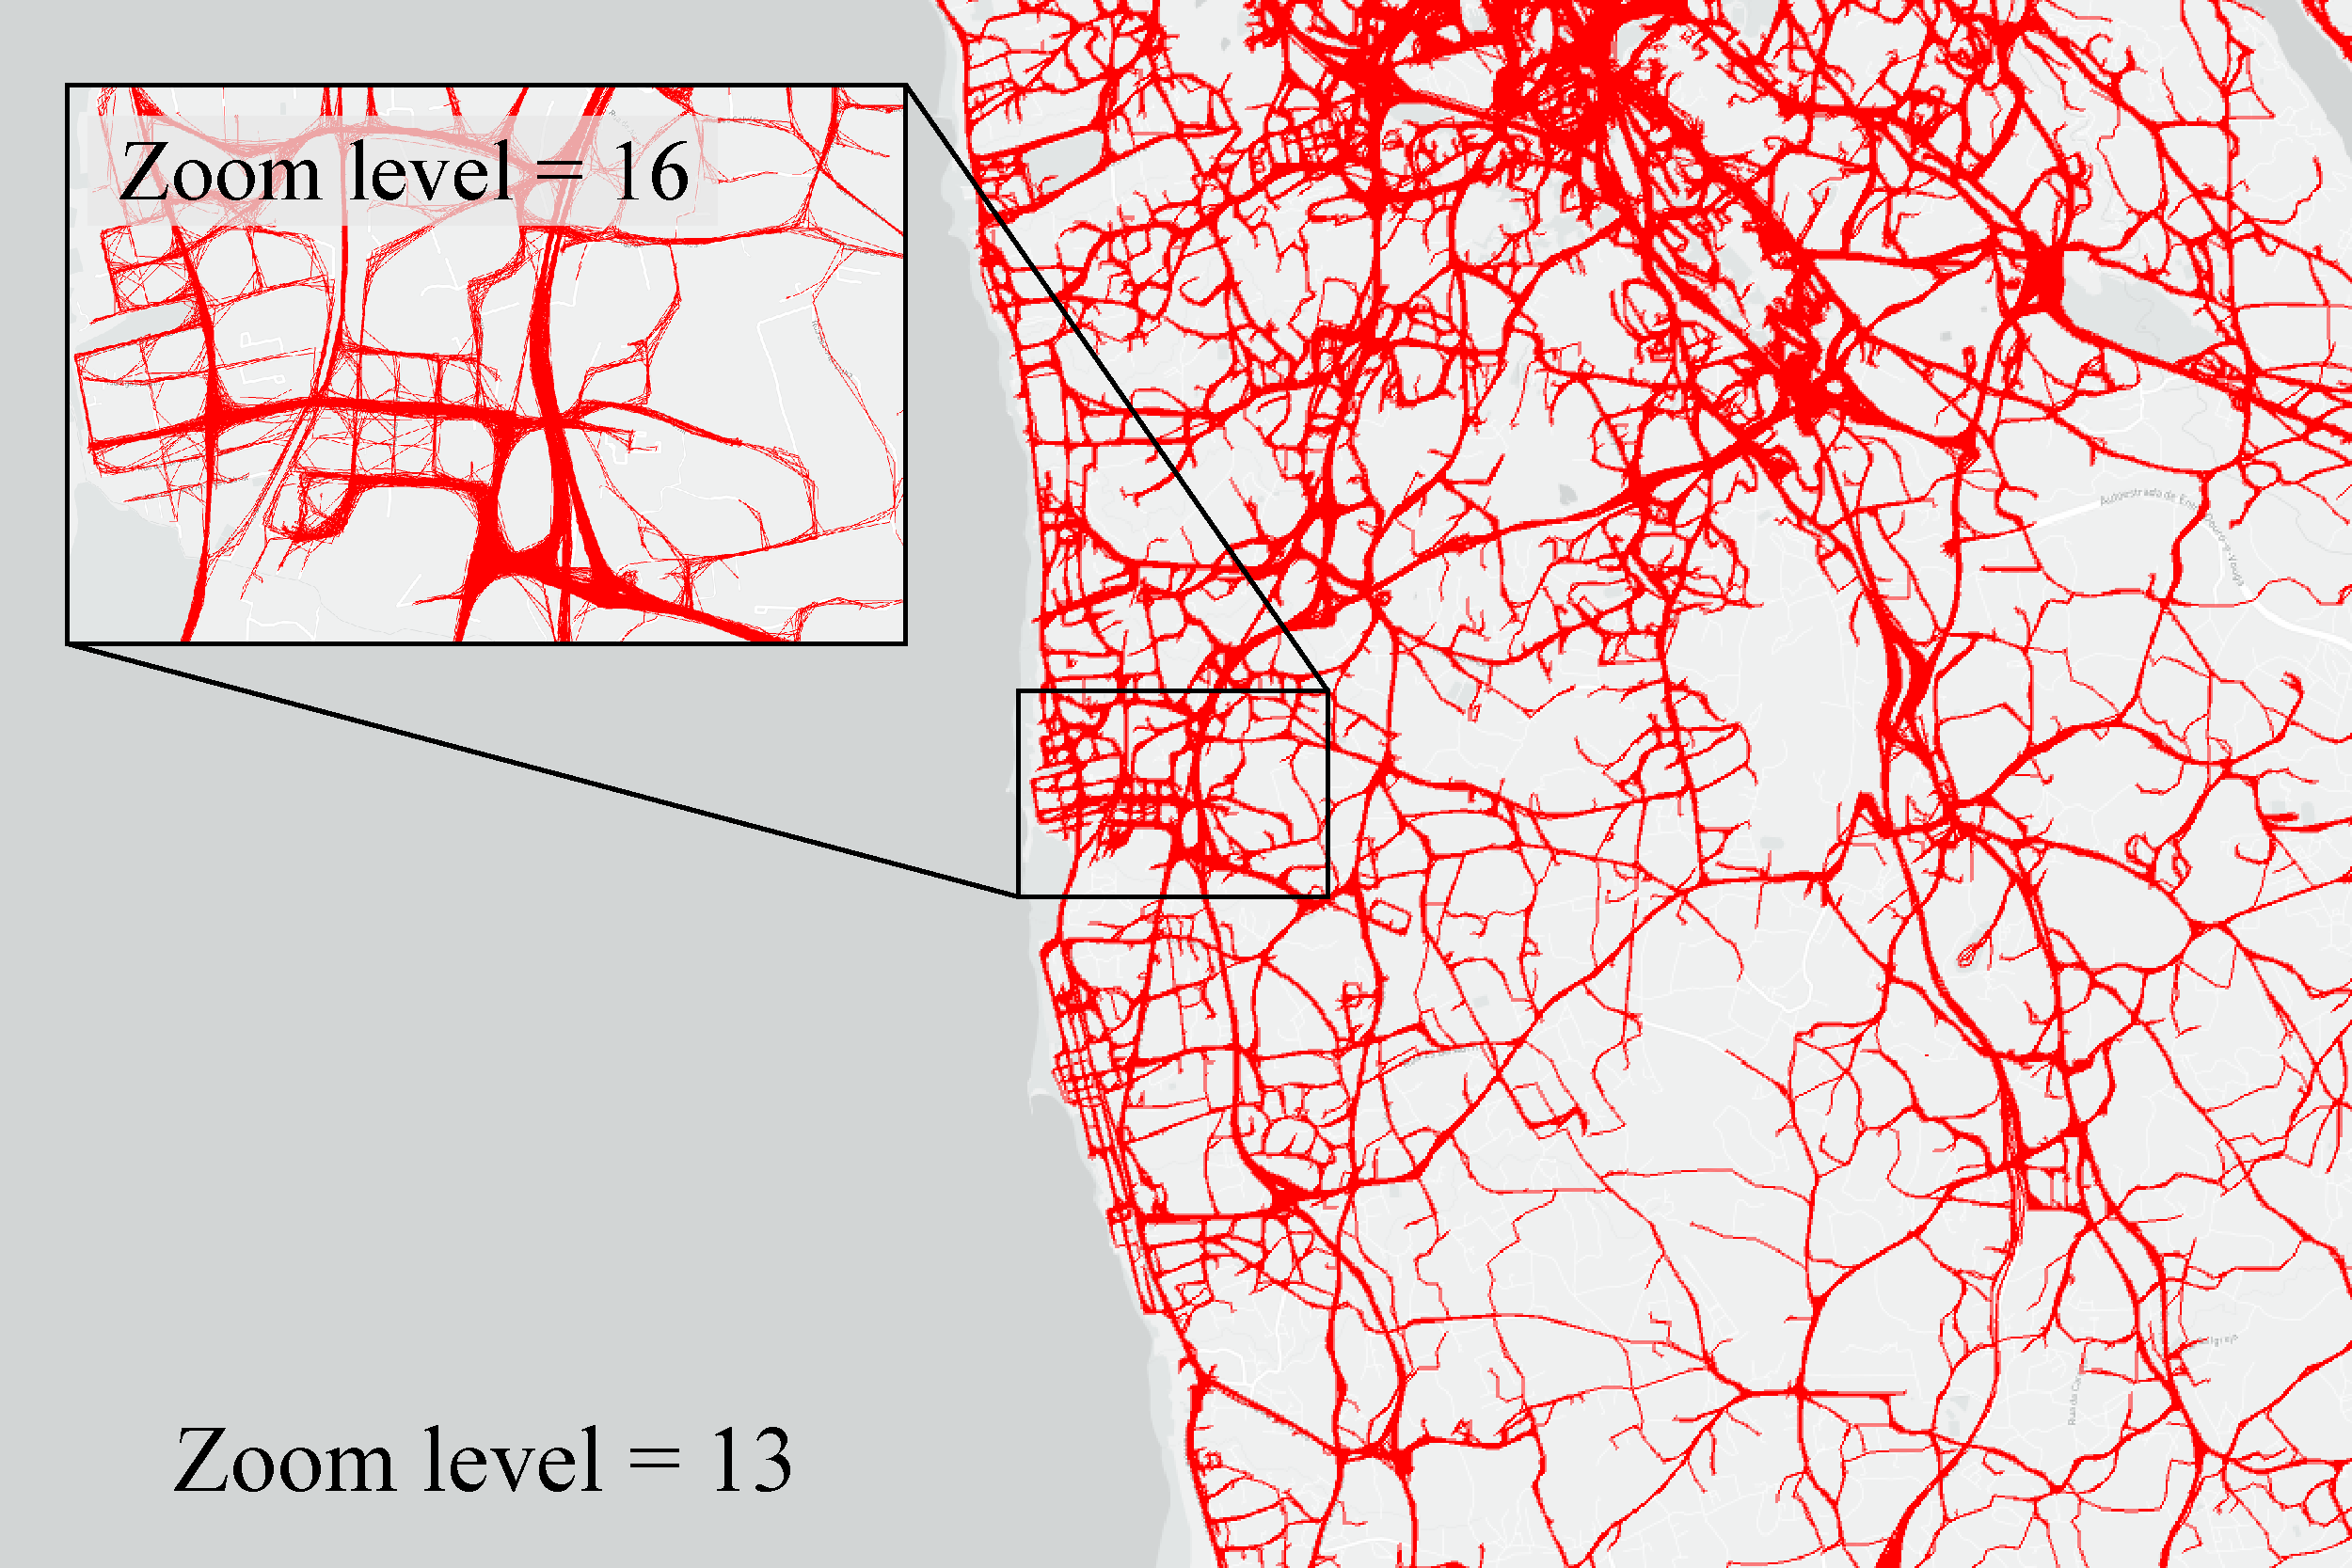
\includegraphics[width=0.73\linewidth]{pictures/zoomlevel.pdf}
     \label{Fig:zoom}
     \trim
     \caption{An illustration of zoom levels.}
   \end{minipage}
   \trim
\end{figure*}


%In the previous section, we presented the $\vats$ algorithm, which produces quality-guaranteed samples and runs efficiently. In this section, we focus on the third technical challenge: \emph{how to tackle the visual clutter problem in large trajectory visualization}?

In this part, we improve $\vats$ by considering (i) trajectory data distribution, and (ii) human perception capability. We elaborate (i) and (ii) by the examples in Figure~\ref{fig:delta}.


\stitle{Trajectory data distribution} Considering the \pt{} trajectory dataset, Figure~\ref{fig:delta}(A) is the visualization result of $\vats$ with sampling rate $0.5\%$.
It is obvious that the trajectories follow a non-uniform distribution, and there are some dense regions and sparse regions as illustrated by the two rectangles in Figure~\ref{fig:delta}(A).
There are many points in the dense region, which creates visual clutter and makes it difficult to identify the main roads.


%Obviously, the real-world trajectory dataset is non-uniform distributed.
%For example, the trajectories in dense region are much more than those in the sparse region, as illustrated by the rectangles in Figure~\ref{fig:delta}(A).

\stitle{Human perception capability} Comparing Figures~\ref{fig:delta}(A) and (B), it is easier to tell their differences in the sparse regions than in the dense regions.
This is because human perception has limited capability, and hence two visualizations look indistinguishable if both of them contain a large number of points in the same area.
The two dense regions look similar although Figure~\ref{fig:delta}(B) contain fewer points in this region than Figure~\ref{fig:delta}(A).
However, for the sparse region, $\vats$ loses some trajectories and it is easy to tell the differences between Figures~\ref{fig:delta}(A) and~\ref{fig:delta}(B).

%\begin{figure*}%[t]
%    \centering
%	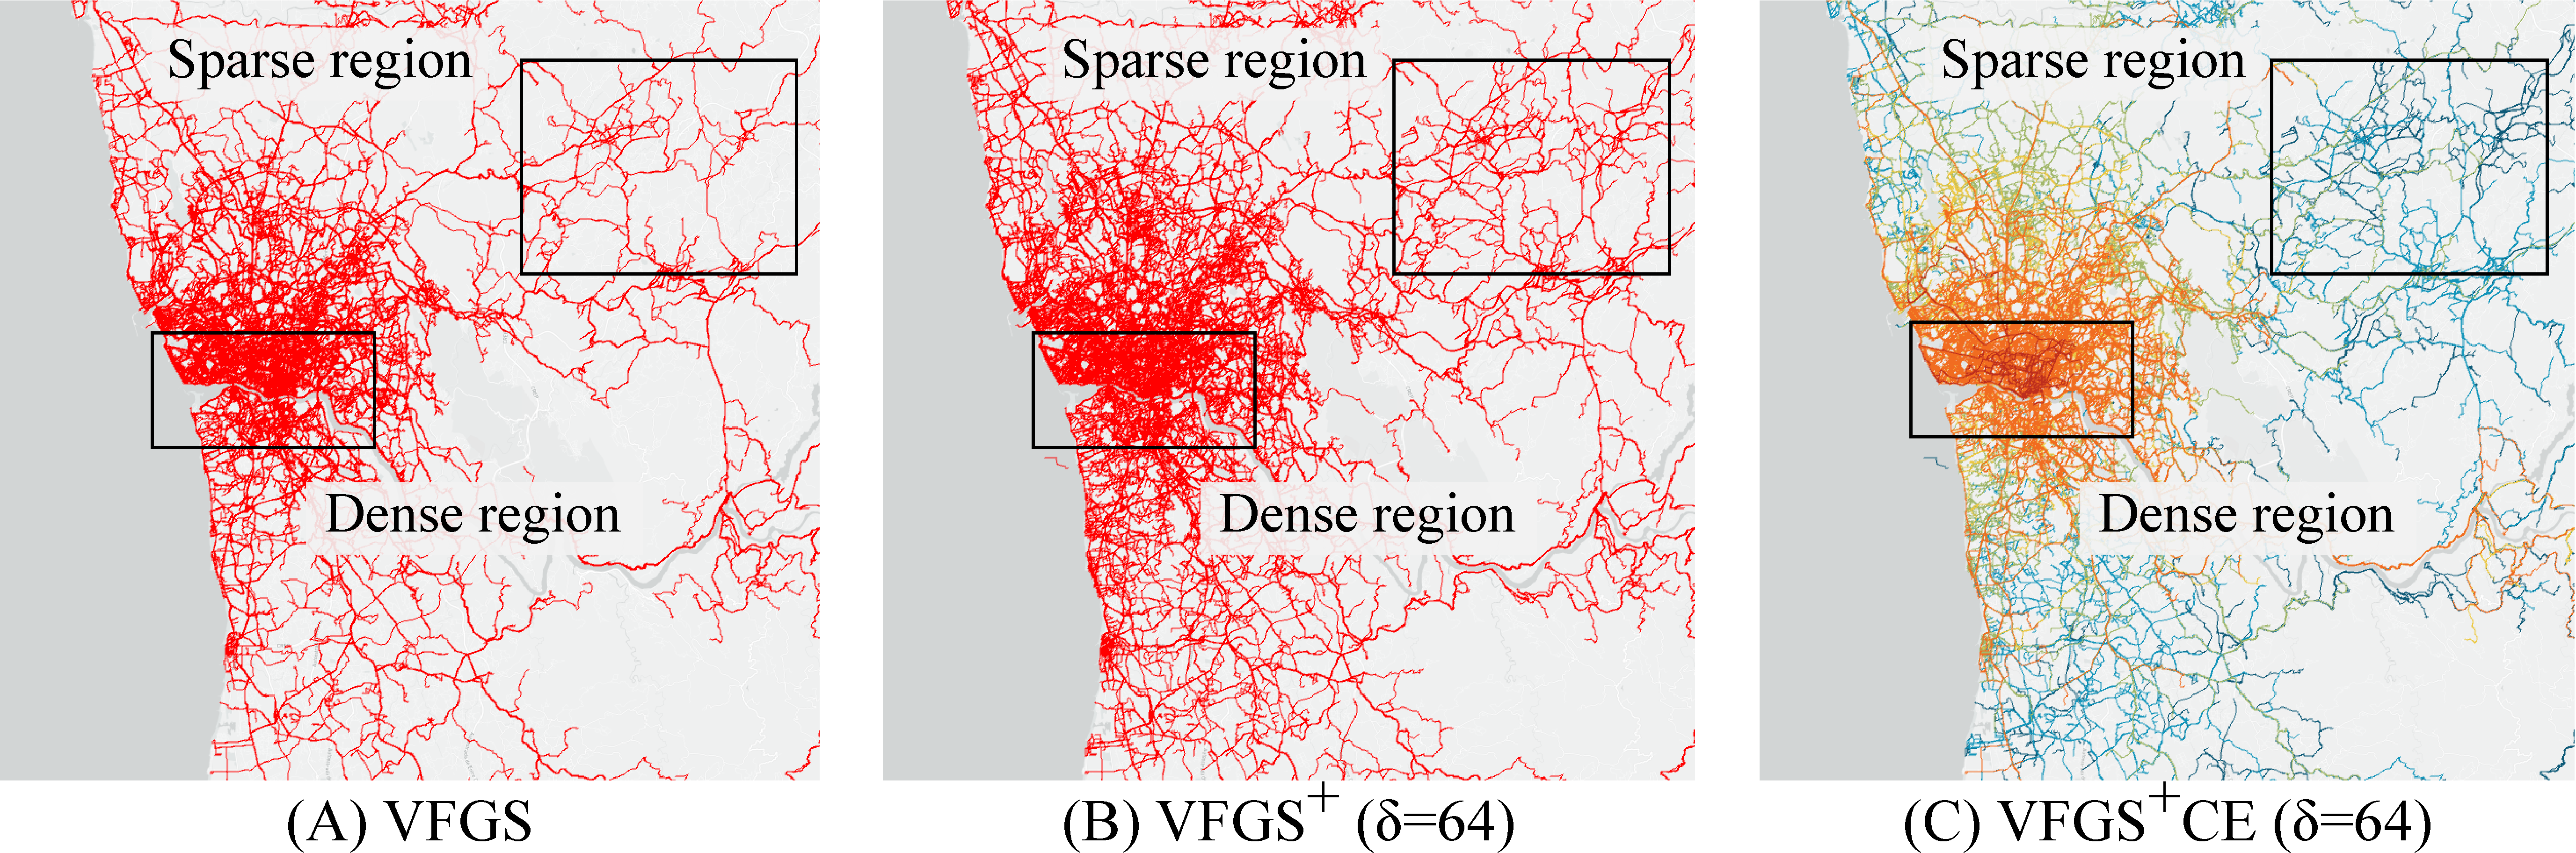
\includegraphics[width=0.7\textwidth]{pictures/problemsolveing/delta_motivation.pdf}
%	\caption{The advanced approach $\vatss$ on \pt{} ($\alpha = 0.5\%$).\Bo{edit figure captions}}\label{fig:delta}
%\end{figure*}


%\begin{table}
%  \begin{tabular}{cc}
%        \begin{figure}%[t]
%	       \centering
%	       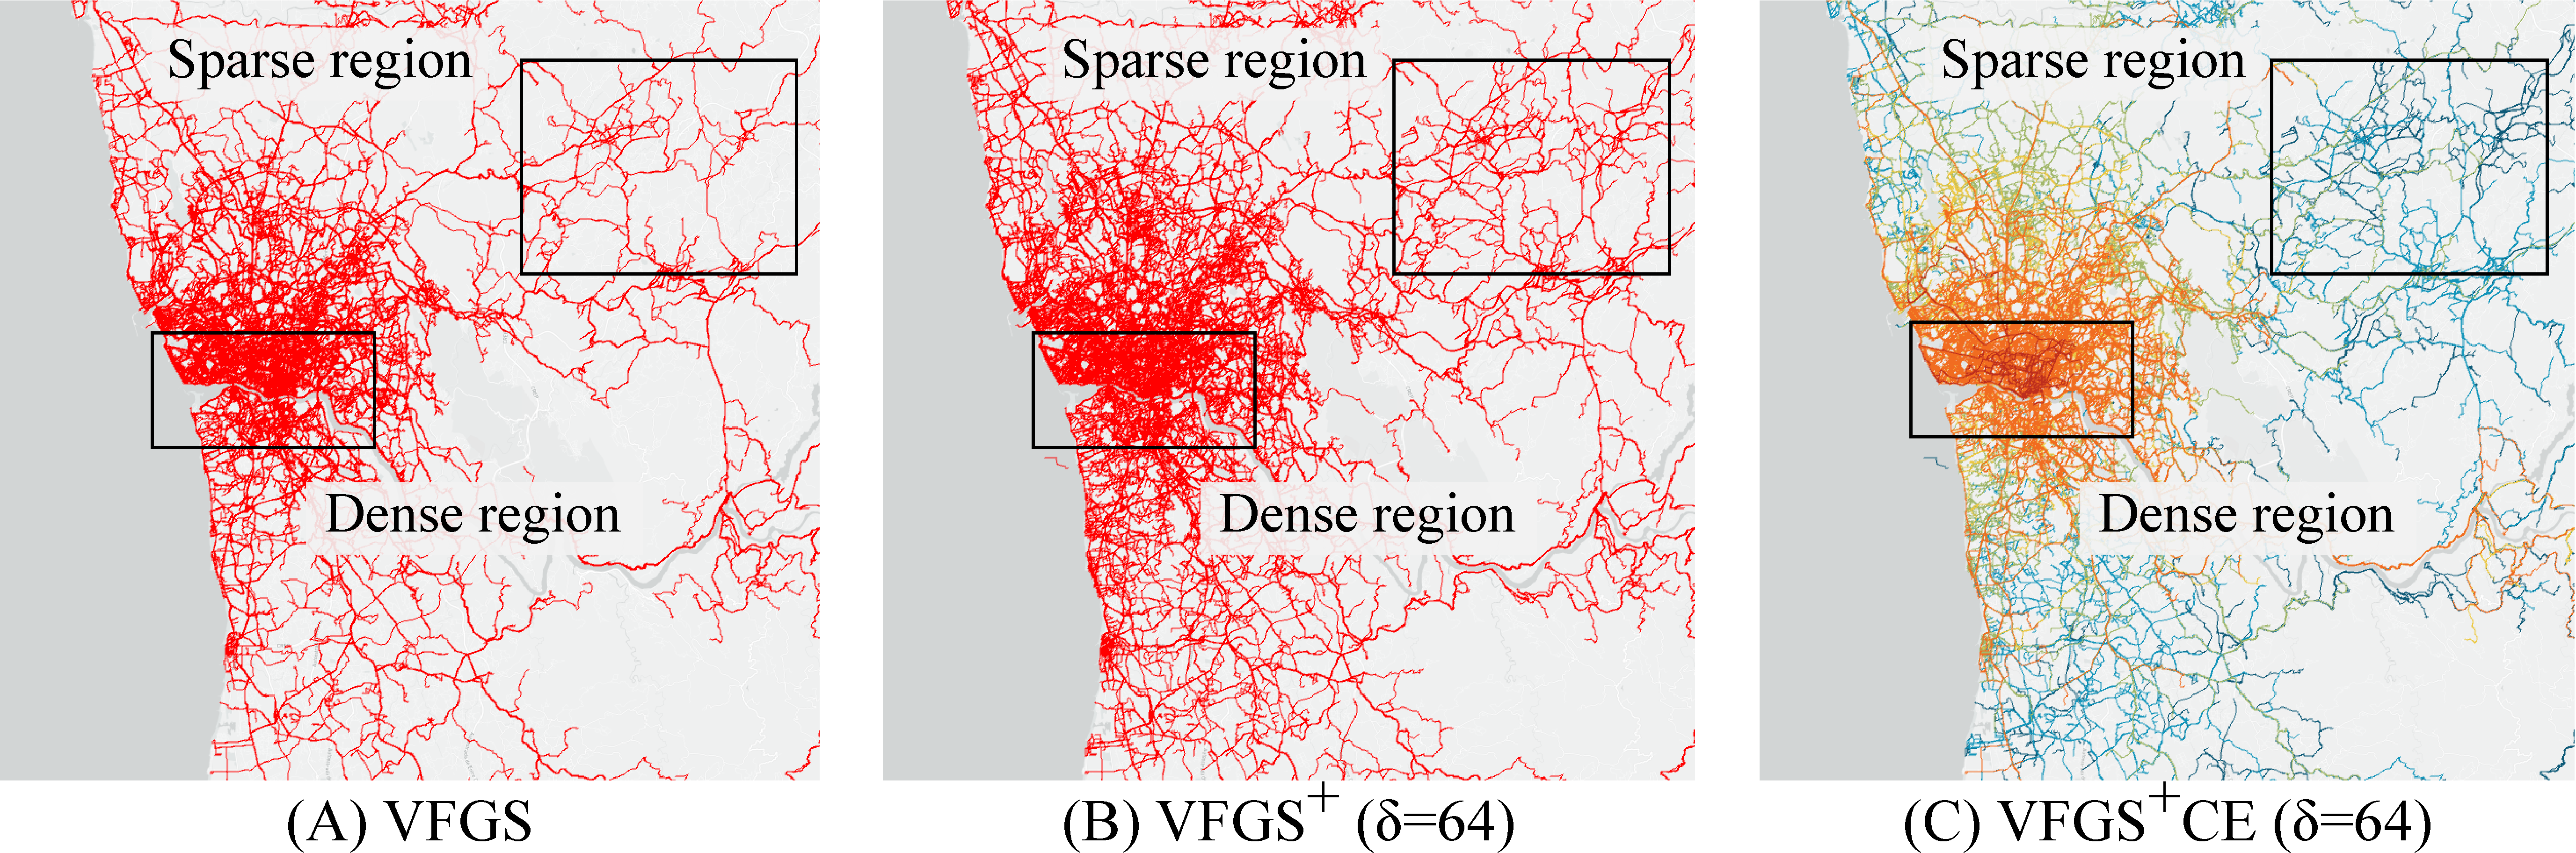
\includegraphics[width=0.7\textwidth]{pictures/problemsolveing/delta_motivation.pdf}
%	       \caption{The advanced approach $\vatss$ on \pt{} ($\alpha = 0.5\%$).\Bo{edit figure captions}}\label{fig:delta}
%        \end{figure}
%      &
%        \begin{figure}[t]
%        	\centering
%        	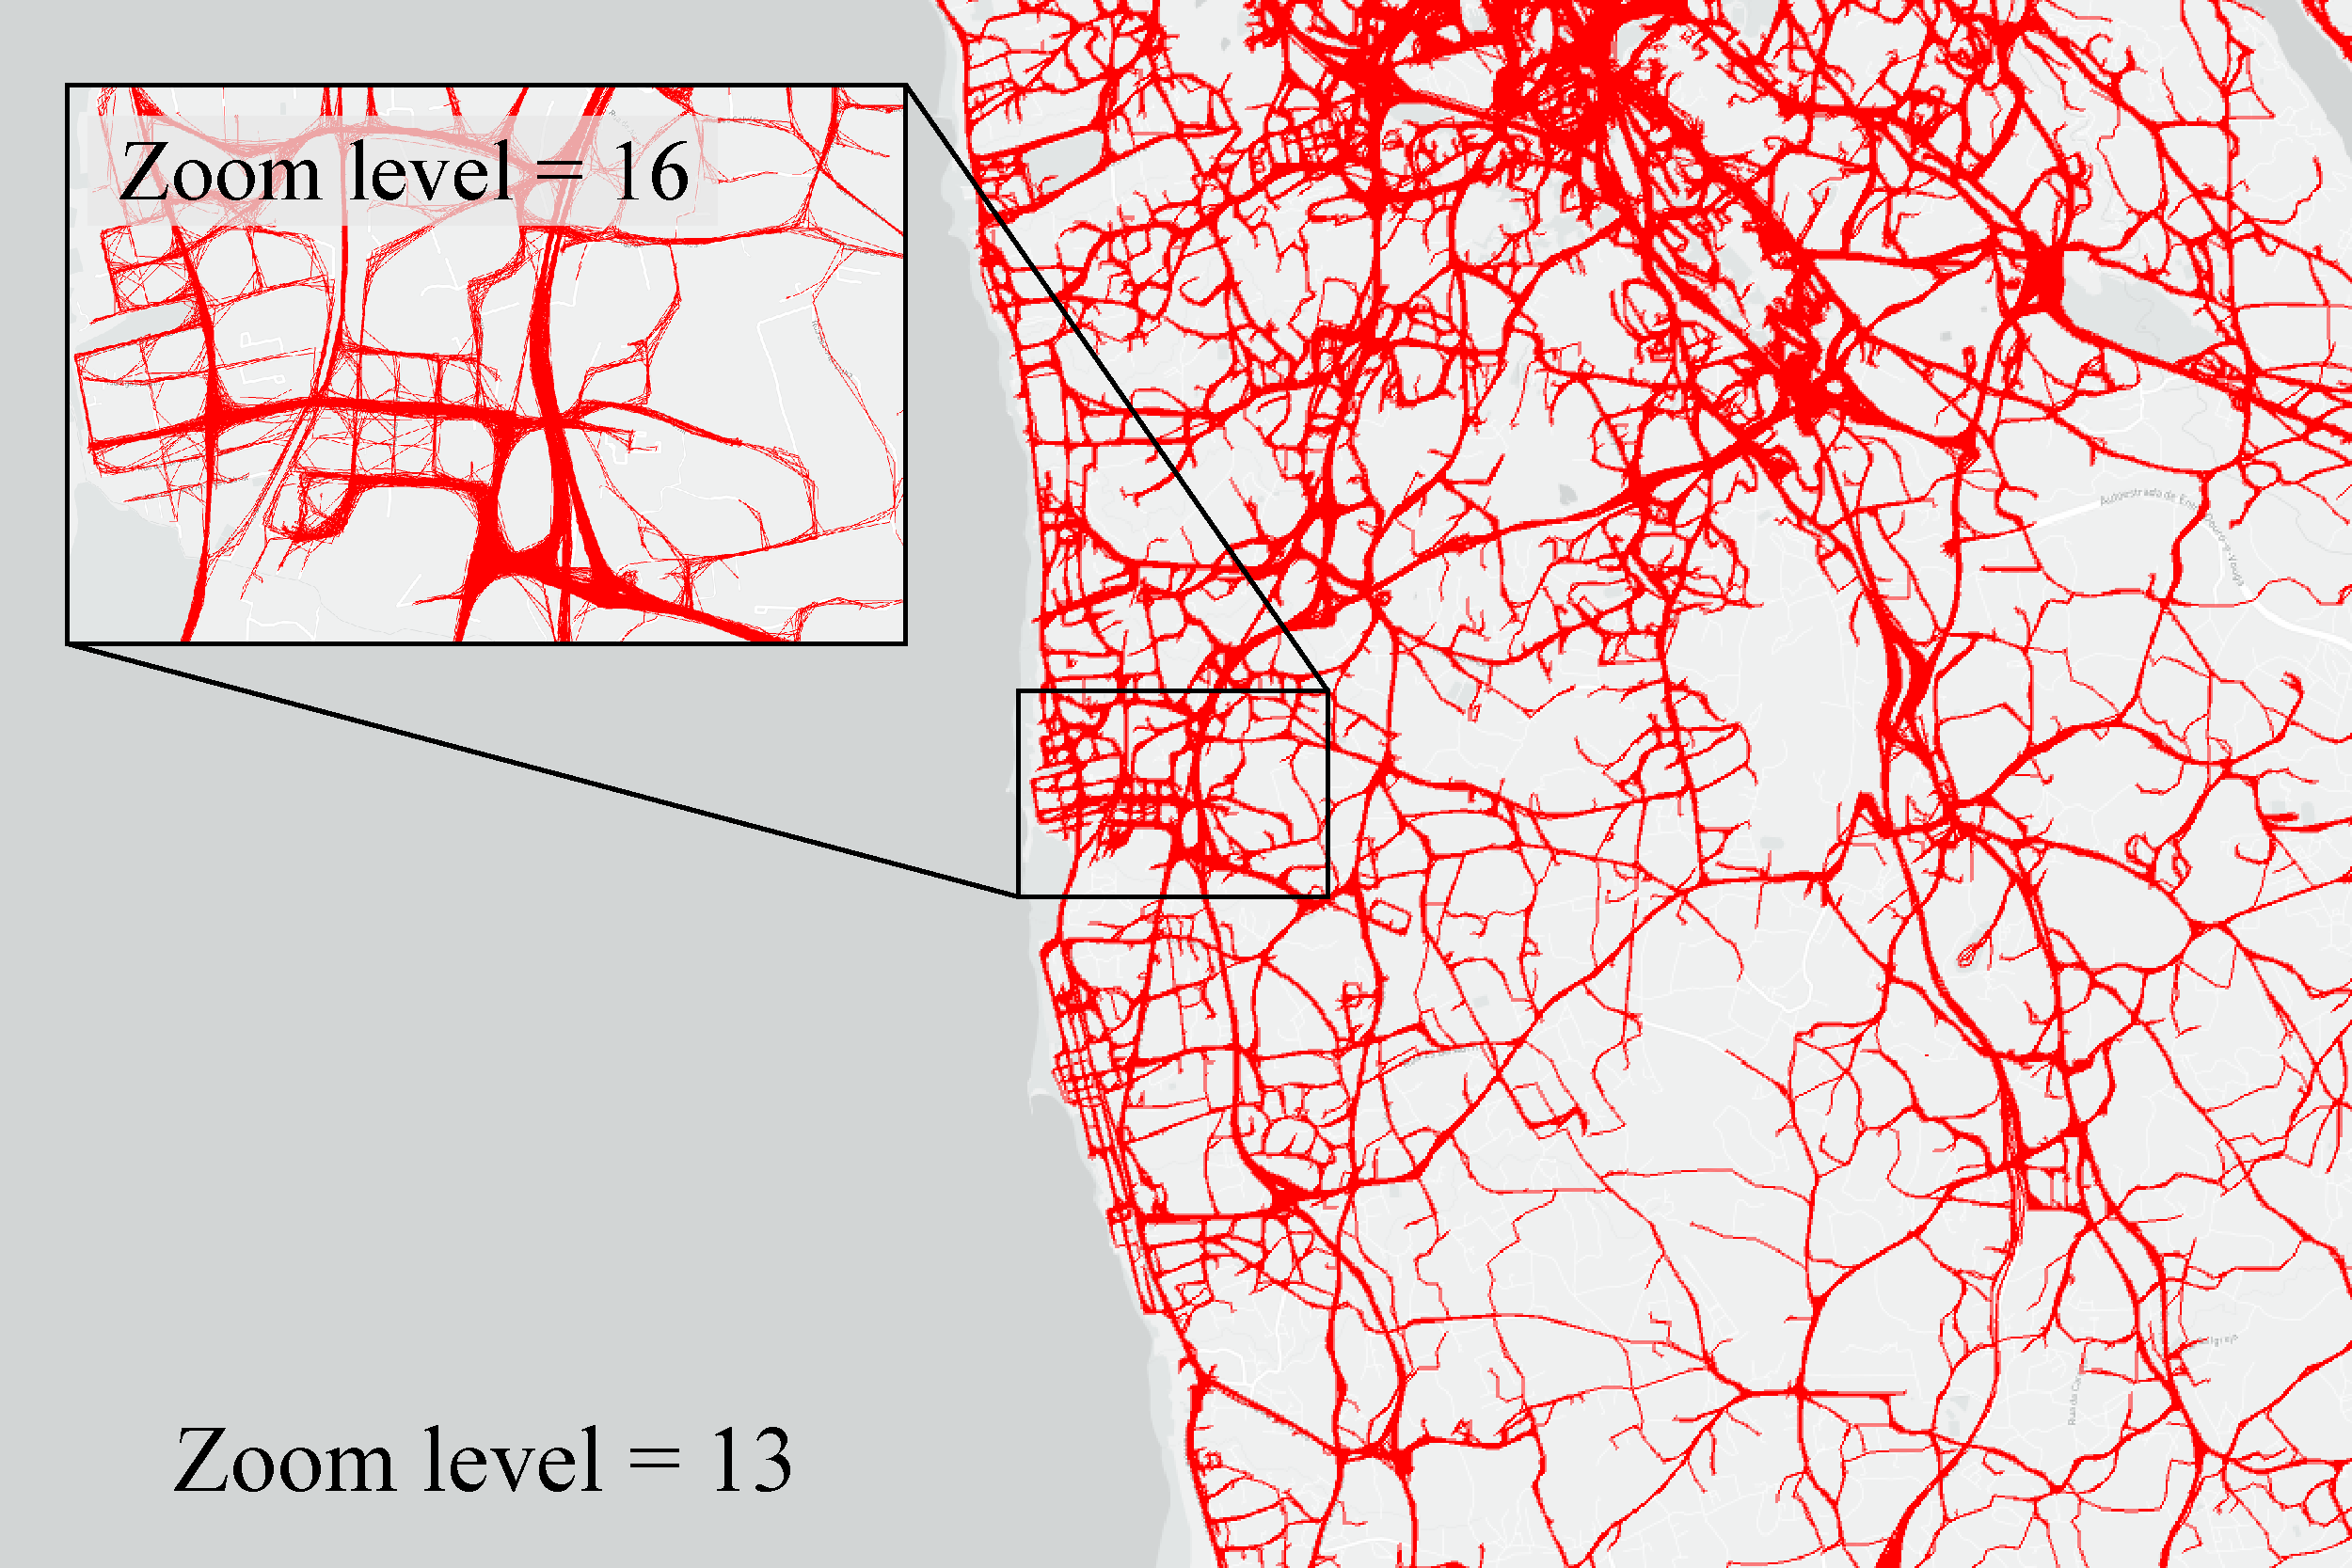
\includegraphics[width=0.3\textwidth]{pictures/zoomlevel.pdf}
%        	\caption{An illustration of different zoom level.}	\label{fig:zoom}
%        \end{figure}
%  \end{tabular}
%\end{table}



%(see Algorithm~\ref{alg:plus})

Based on the two observations above, we can improve  $\vats$ by delivering richer information in the sparse regions and reducing visual clutter in the dense regions.
$\vatss$ in Algorithm~\ref{alg:plus} achieves both objectives using a perception tolerance parameter $\delta$, which models the perception capability of human.
Specifically, if pixel $(x,y)$ in the canvas is marked by the result set $\oR$,
the pixels around $(x,y)$, i.e., from $(x-\delta, y-\delta)$ to $(x+\delta, y+\delta)$, do not need to be marked as they are close to $(x,y)$ and human perception cannot tell nearby pixels apart. We modify $\vats$ in Algorithm~\ref{alg:greedy} to incorporate the perception tolerance parameter $\delta$ in Algorithm~\ref{alg:plus}.
$\vatss$ measures the contribution of each trajectory $t_i$ w.r.t. the augmented visualized point set $\VV(\oR)^{+}$ in Line~\ref{line:deltamax},
where $\VV(\oR)^{+}$ includes both pixels on the selected trajectories and their tolerance pixels (in Line~\ref{line:delta}).
We also use the heap-based lazy computation to speedup $\vatss$.


%Taking the above two observations into consideration, we can further improve the returning result of visual quality-guaranteed sampling approach $\vats$ by
%delivering rich information at sparse regions and reducing visual clutter in dense regions.
%In this section, we devise the advanced approach $\avats$ (see Algorithm~\ref{alg:plus}) to achieve the above two objectives.
%In specific, we introduce perception tolerance parameter $\delta$ in $\avats$, which models the perception capability of humans at the highest level of details.
%In other words, suppose the pixel $(x,y)$ in canvas is covered by the result set $\oR$ at the highest level,
%the pixels around $(x,y)$, i.e., from $(x-\delta, y-\delta)$ to $(x+\delta, y+\delta)$, are not necessary to cover because they are in the perception tolerance of human beings.


%It measures the contribution of each trajectory $t_i$ w.r.t the selected trajectory set $\oR$'s augmented set $\oR^{+}$, i.e., the selected trajectories and their tolerance pixels.
%.
%The augmented set $\oR^{+}$ will be updated by the selected trajectory $tmp$ and its tolerance pixels set (in Line~\ref{line:delta}).

%
\begin{algorithm}
    \caption{$\vatss(\D,k=\lceil \alpha \mathcal{T} \rceil,\delta)$} \label{alg:plus}
    \begin{algorithmic}[1]
    \State Initialize result set $\oR \leftarrow \emptyset$
    \State Initialize augmented result set $\oR^{+} \leftarrow \emptyset$
    \While{$|\oR| < k$}
        \State $\mathsf{tmp} \leftarrow \arg\max_{t_i \in \D} | t_i  \cup \VV(\oR)^{+} |$ \label{line:deltamax}
        \State $\oR \leftarrow \oR \cup \{ \mathsf{tmp} \}$
        \State $\VV(\oR)^{+} \leftarrow \VV(\oR)^{+} \cup \mathsf{augment}(\mathsf{tmp}, \delta)$\label{line:delta}
    \EndWhile
    \For{each $t$ in $\D$} \Comment{Representative encoding} \label{line:s}
        \State $tr \leftarrow \arg\min_{t_i \in \oR}{|t-\mathsf{augment}(t_i, \delta)|}$
        \State $tr.\mathsf{cnt}++$ \label{line:e}
    \EndFor
    \State Return $\oR$
    \end{algorithmic}
\end{algorithm}


%Interestingly, the visual clutter large trajectory visualization problem can be further reduced
%by encoding representative trajectories in $\oR$ (the returning result of $\avats$) with colors.
%In particular, $\avats$ selects the trajectory with the largest uncovered pixels by taking the perception tolerance capability of humans into account at each iteration,
%instead of only choosing the trajectory with the largest uncovered pixels in $\vats$ (Algorithm~\ref{alg:greedy}).


$\vatss$ in Algorithm~\ref{alg:plus} selects trajectories with good representativeness and some trajectories will not be included into the result set $\oR$ even though they have more uncovered pixels w.r.t. $\oR$.
The reason is that their uncovered pixels are too close to the pixels in the selected trajectories (i.e., within the tolerance area of selected pixels).
Compared with $\vats$, $\vatss$ is more likely to sample trajectories in the sparse regions as their pixels are less likely to be covered by other trajectories as shown in Figure~\ref{fig:delta}.
Moreover, reducing the number of trajectories sampled from the dense regions helps to reduce visual clutter.


%Take Figure~\ref{fig:zoom}(A) for example, suppose $\delta=1$ and trajectory $a$ was selected at the first iteration, the trajectory to select in the second iteration is $c$ instead of $b$ because almost all pixels in $b$ is in the tolerance area of $a$'s.

%\begin{figure}[t]
%	\centering
%	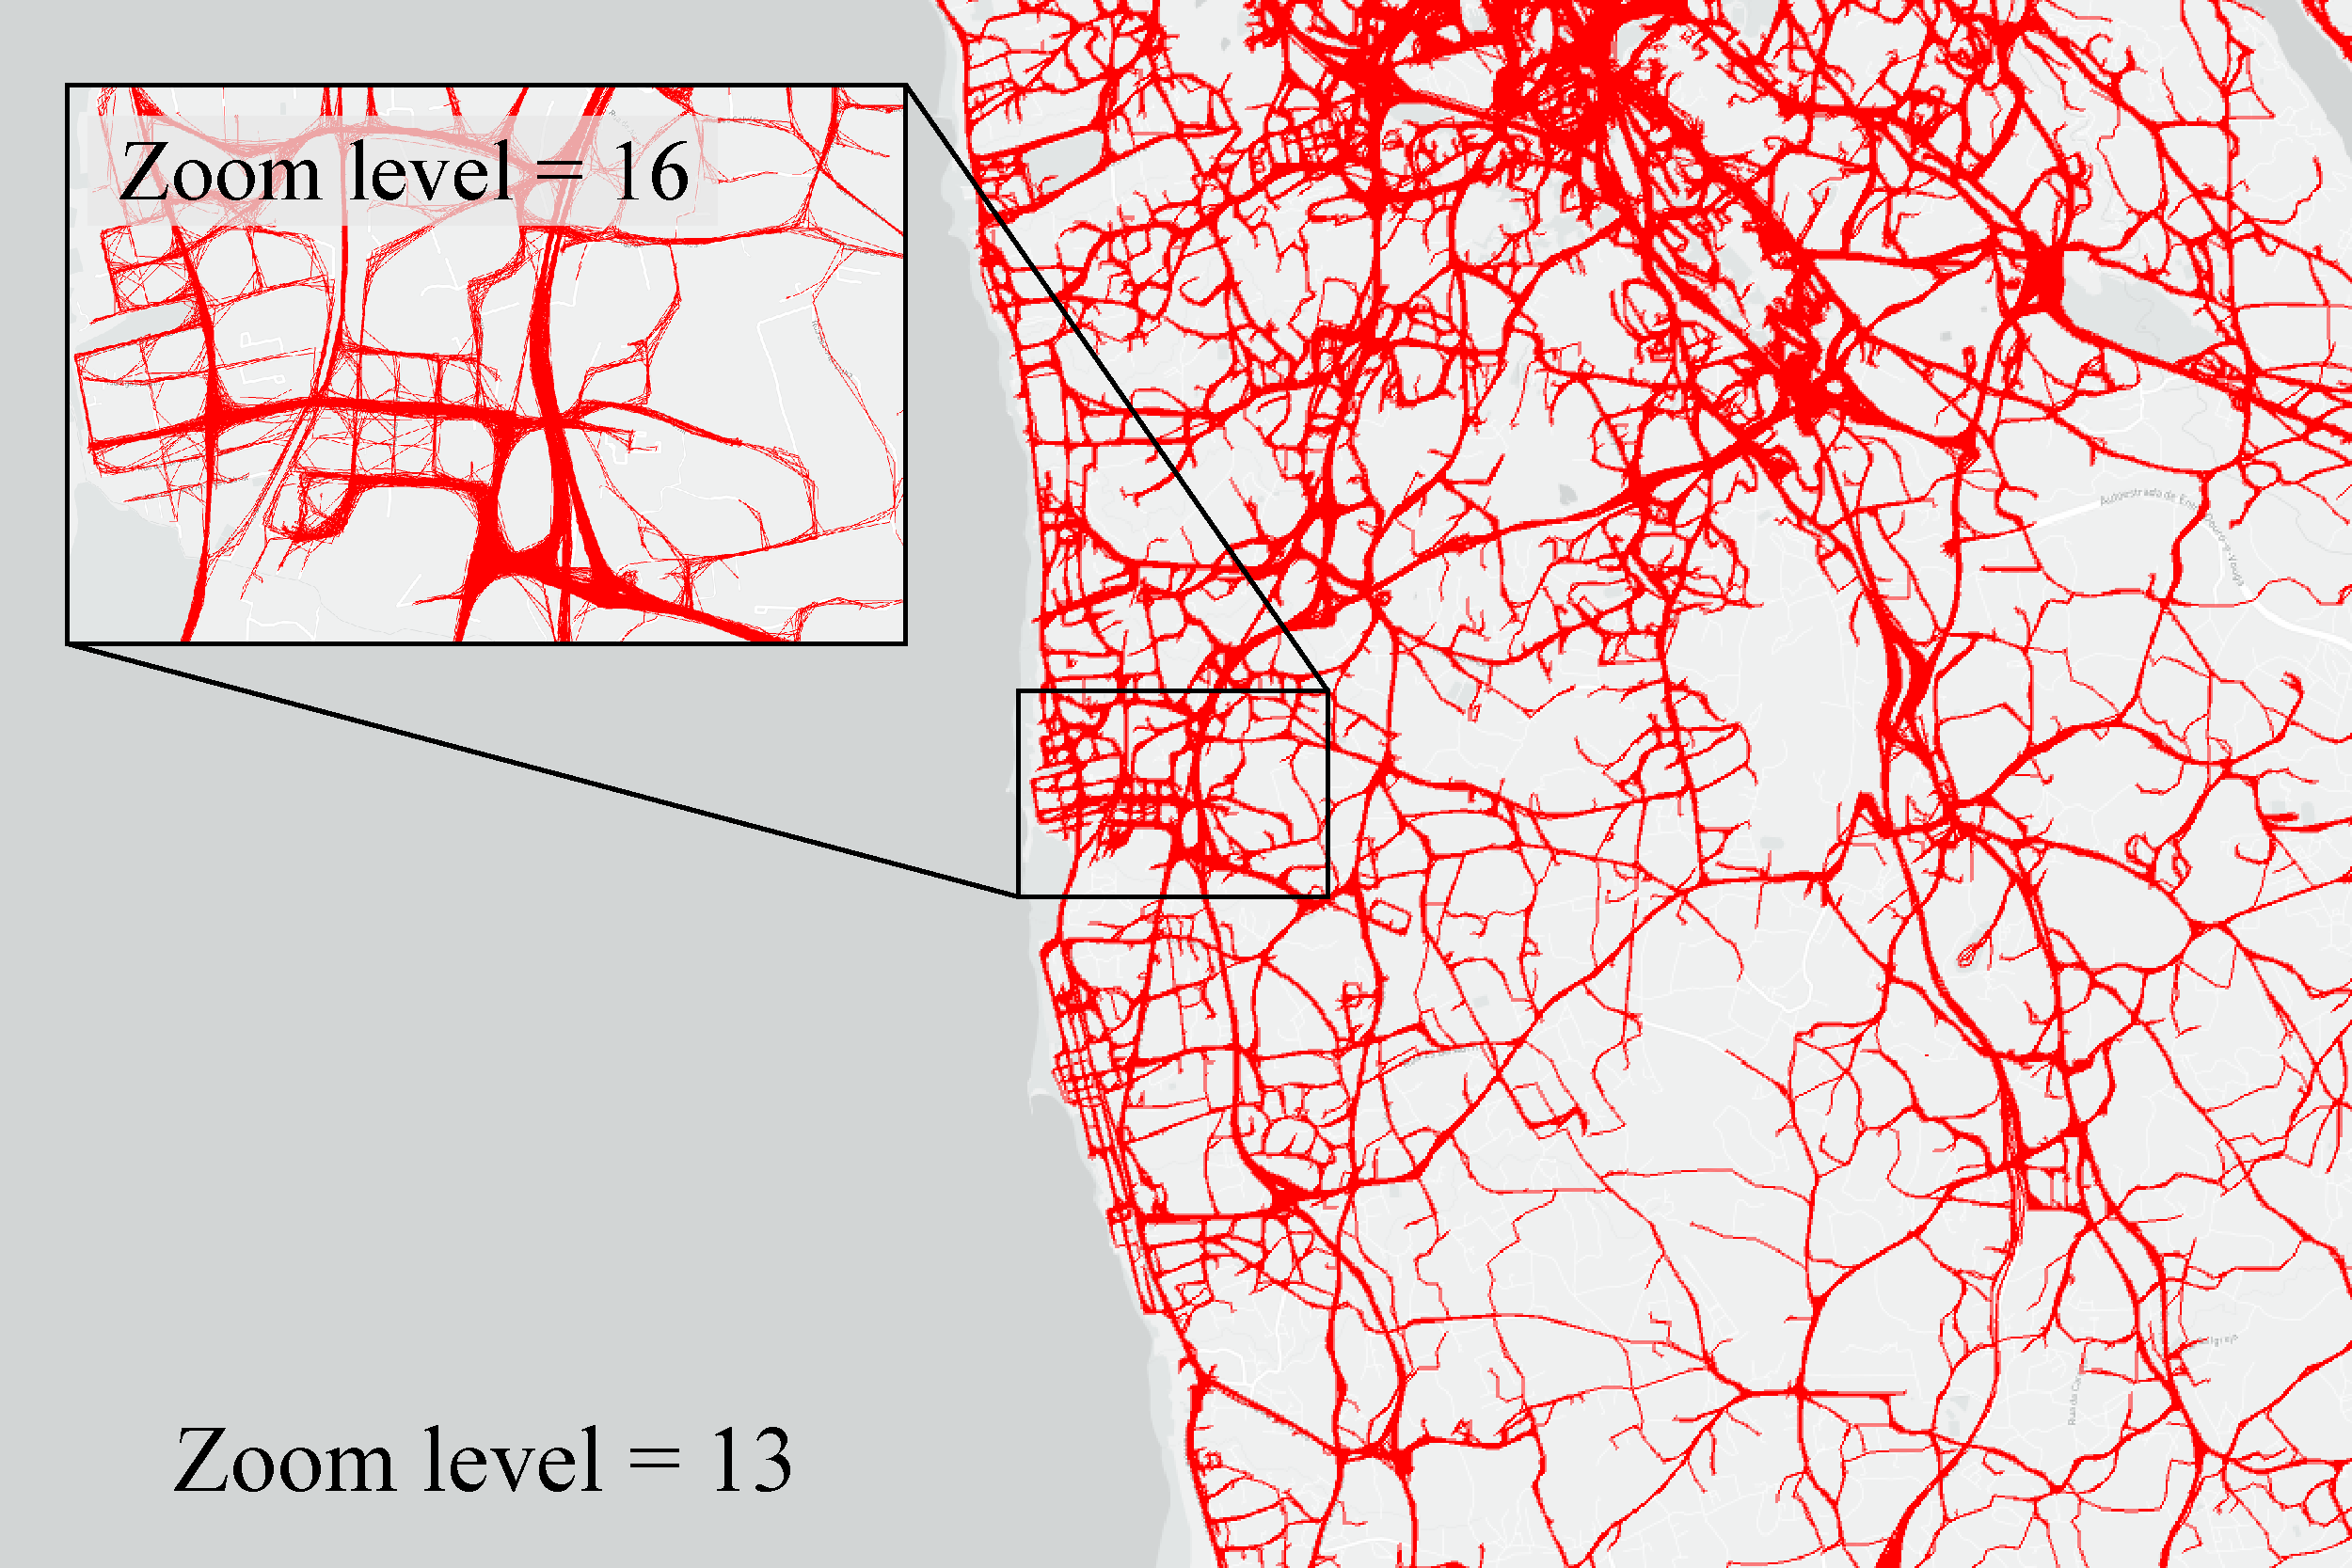
\includegraphics[width=0.3\textwidth]{pictures/zoomlevel.pdf}
%	\caption{An illustration of different zoom level.}	\label{fig:zoom}
%\end{figure}


One subtlety is that different $\delta$ needs to used for different \emph{zoom levels} (or regions with different sizes).
For example, Google map~\cite{googlemap} provides zoom levels from 0 to 20, with level 0 providing the largest visualization range (i.e., the whole world) but the lowest resolution, and level 20 providing the smallest visualization range (e.g., individual building) but the highest resolution.
We provided an illustration of zoom level in Figure 6 and users may select different zoom levels for visualization according their needs.
Note that we define $\delta$ on the highest zoom level (i.e., using the raw distance of the locations) to account for different resolutions.
If the zoom level is small (i.e., the visualization region is large), we can apply a large $\delta$ because locations with a large raw distance look close to each other in the visualization and we can afford to lose more details.
If the zoom level is large (i.e., the visualization region is small), we need to use a small $\delta$ as users typically want to investigate some fine-grained details in this case and using a large $\delta$ will lose these details.

%We will elaborate this point shortly in experimental section.

%Therefore, we use different $\delta$ for different zoom levels accordion to Table~\ref{tab:delta}, which was obtained empirically from a user evaluation of the visualization results.
%\begin{table}
%	\centering
%	\small
%	\caption{Values of $\delta$ for different zoom levels}
%	\begin{tabular}{|c|c|c|c|c|} \hline
%		\textbf{Zoom Level} &  &  &  & \\
%		\hline
%		$\delta$ &  &  & &  \\ \hline
%	\end{tabular}	\label{tab:delta}
%\end{table}

%Ideally, we want a sample to be \textit{zoom-level-independent}, providing a consistent quality guarantee at different zoom levels. This turns out to be straightforward as trajectory visualization merges several pixels in a high-level result (by pixel-wise $OR$) to obtain a pixel in a lower-level visualization result. The following theorem shows that it suffices to satisfy the quality guarantee at the highest zoom level.

%$\delta$ for different zoom levels, user study smaller delta for higher zoom levels


%$\vatss$ also provides excellent visual quality at arbitrary zooming resolutions. This is because it considers the perception tolerance parameter $\delta$  at the highest zoom level. For example, the zoom level in Figure~\ref{fig:zoom}(A) is higher than that in Figure~\ref{fig:zoom}(B). According to our elaboration, $\vatss$ selects trajectory $a$ and $c$ for Figure~\ref{fig:zoom}(A). When the area is zoomed out, as shown in Figure~\ref{fig:zoom}(B), trajectory $a$ and $c$ still captures the main sketch of the underlying dataset (as gray cells shown).


\stitle{Color encoding scheme}
The visual clutter problem for large-scale trajectory visualization can be further alleviated by encoding the representativeness of the trajectories in $\oR$ with colors.
We define the representativeness of a trajectory $t_i$ as the size of its \emph{reverse nearest neighbor set}, which contains the trajectories in $\D$ that has $t_i$ as its nearest neighbor in $\oR$.
The distance between trajectory $t$ and $t_i$ is defined as the number of pixels in $t$ that can not be covered by the augmented pixels of $t_i$.
We compute the representativeness of each trajectory in $\oR$ in Lines~\ref{line:s}-\ref{line:e} in Algorithm~\ref{alg:plus}.
Figure~\ref{fig:delta}(C) shows the visualization result by encoding trajectories with larger representativeness with warmer colors, for which the main roads in the dense region is clearer than Figure~\ref{fig:delta}(B) with very warm colors.

%There are more details in the sparse regions compared with the $\vats$ result in Figure~\ref{fig:delta}(A), and we can identify the main roads in the dense region with very warm colors.

%Thus, the selected trajectories in the dense region are more representative than those in sparse region.



%		&
%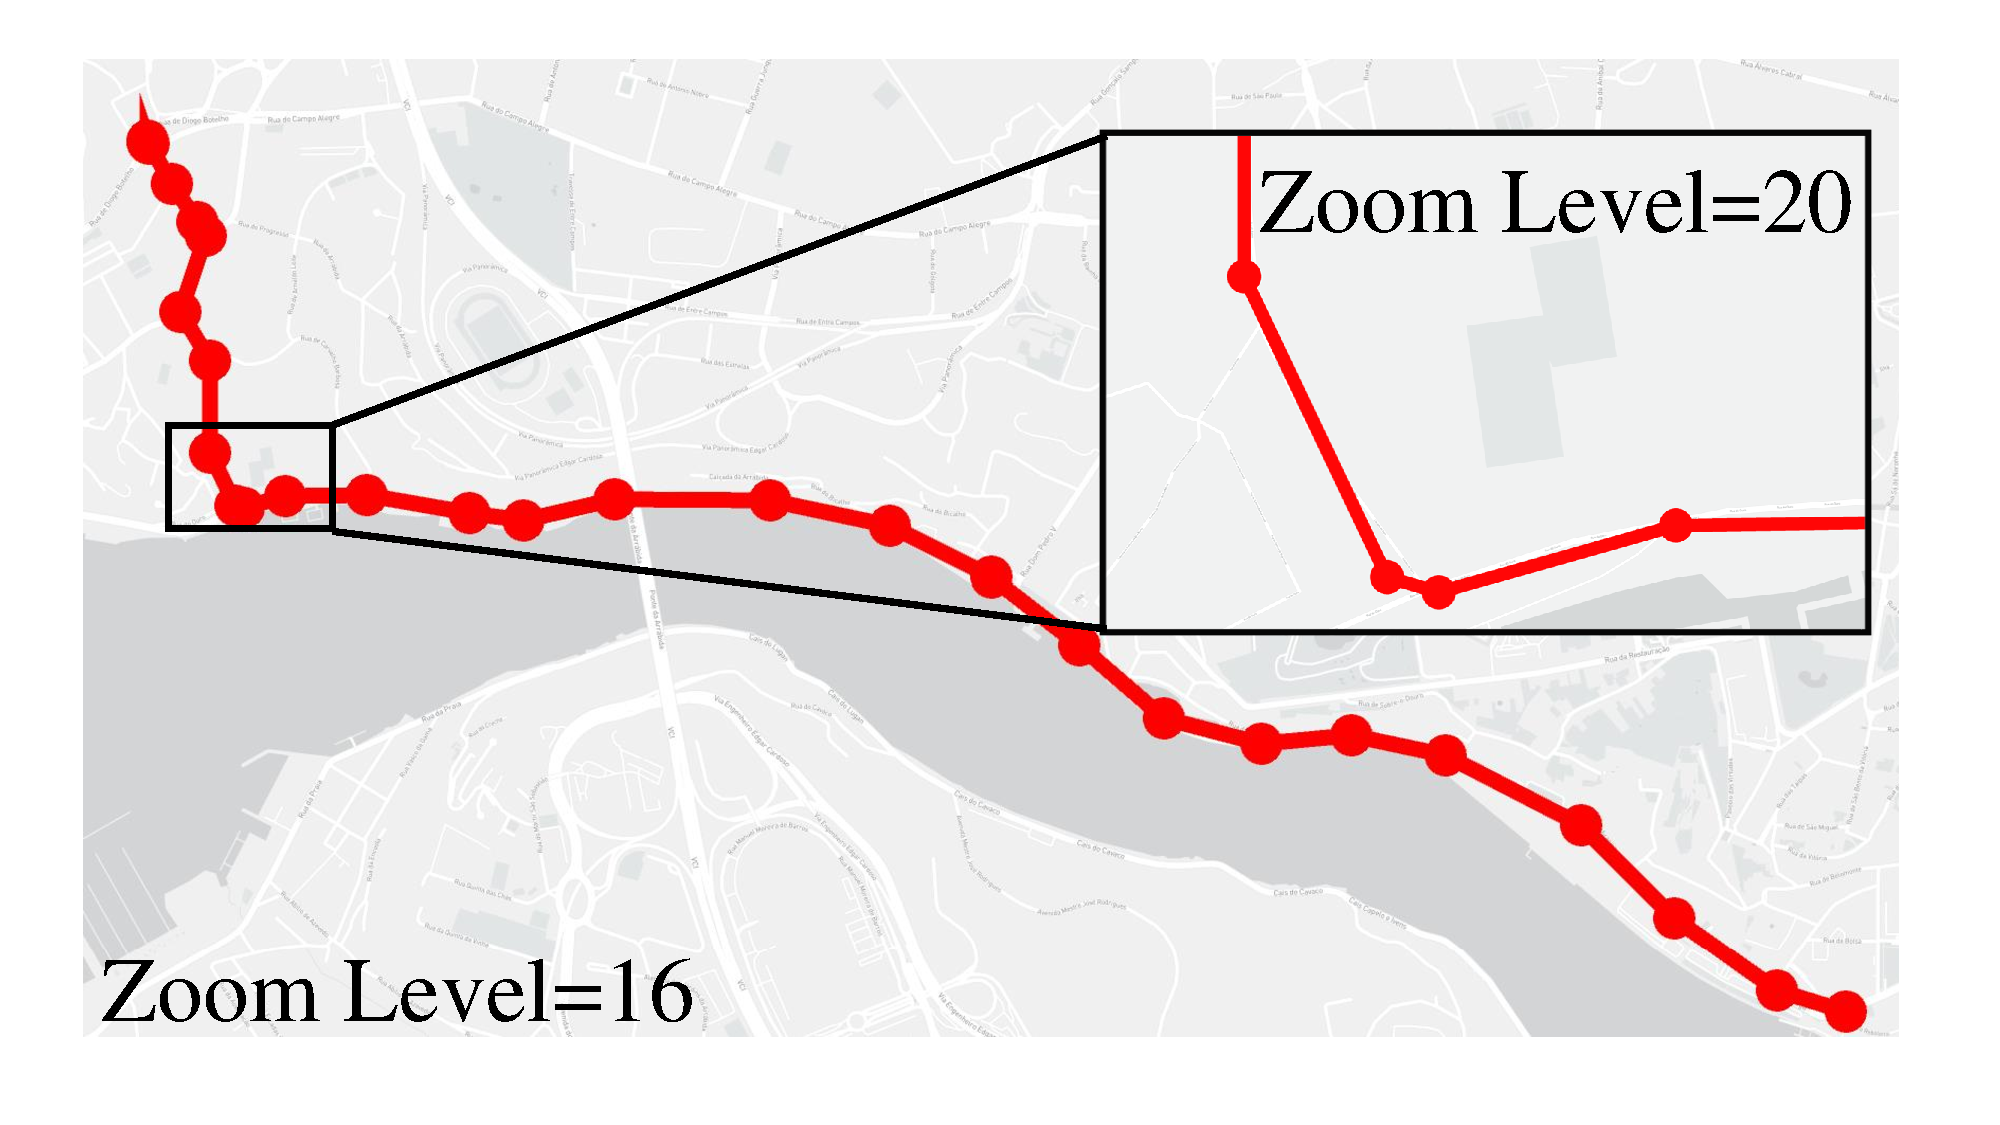
\includegraphics[width=0.48\columnwidth]{pictures/problemsolveing/TrajZoomIn}		
%\\
%(A) Line-based visualization
%&
%(B) Zoom levels


%(1) Richer Information Delivering: details aware; so Arbitrary zooming resolutions
%(2) Popularity Embedding: visual clutter



%\subsection{One-to-many strategy}~\label{sec:one_to_many}
%Since we detect the covered pixels in the highest level, two trajectories may be very close to each other but share very few pixels, which will lead to more information loss in the low zoom view as figure~\ref{fig:one_to_many}.
%We next elaborate a ``one-to-many'' strategy to further optimize the visual quality of our proposed technique.
%Recalling we use the highest zoom level to define the pixel size in the canvas.
%Thus, our visual quality guaranteed sampling algorithm is zoom-level oblivious, e.g., it guarantees the visual quality of result set $\oR$ at every zoom level.
%However, users always do not use/need the highest zoom level in visualization applications.
%For example, Google map shows city and streets at zoom level 1 and 15, respectively~\footnote{\url{https://developers.google.com/maps/documentation/}}.
%Motivated by the above observation, we devise ``one-to-many'' strategy by introducing a visual tolerance parameter $\delta$ to optimize the visual quality for users.
%Specifically, ,
%the ``one-to-many'' strategy will ignore all the pixels around $(x,y)$ within $\delta$ offset distance, i.e., all pixels from $(x-\delta, y-\delta)$ to $(x+\delta, y+\delta)$ will be skipped.
%We will demonstrate the effectiveness of the visual tolerance $\delta$ in experimental evaluations.
%
%%https://developers.google.com/maps/documentation/maps-static/dev-guide#Zoomlevels
%\begin{figure}[t]
%	\centering
%	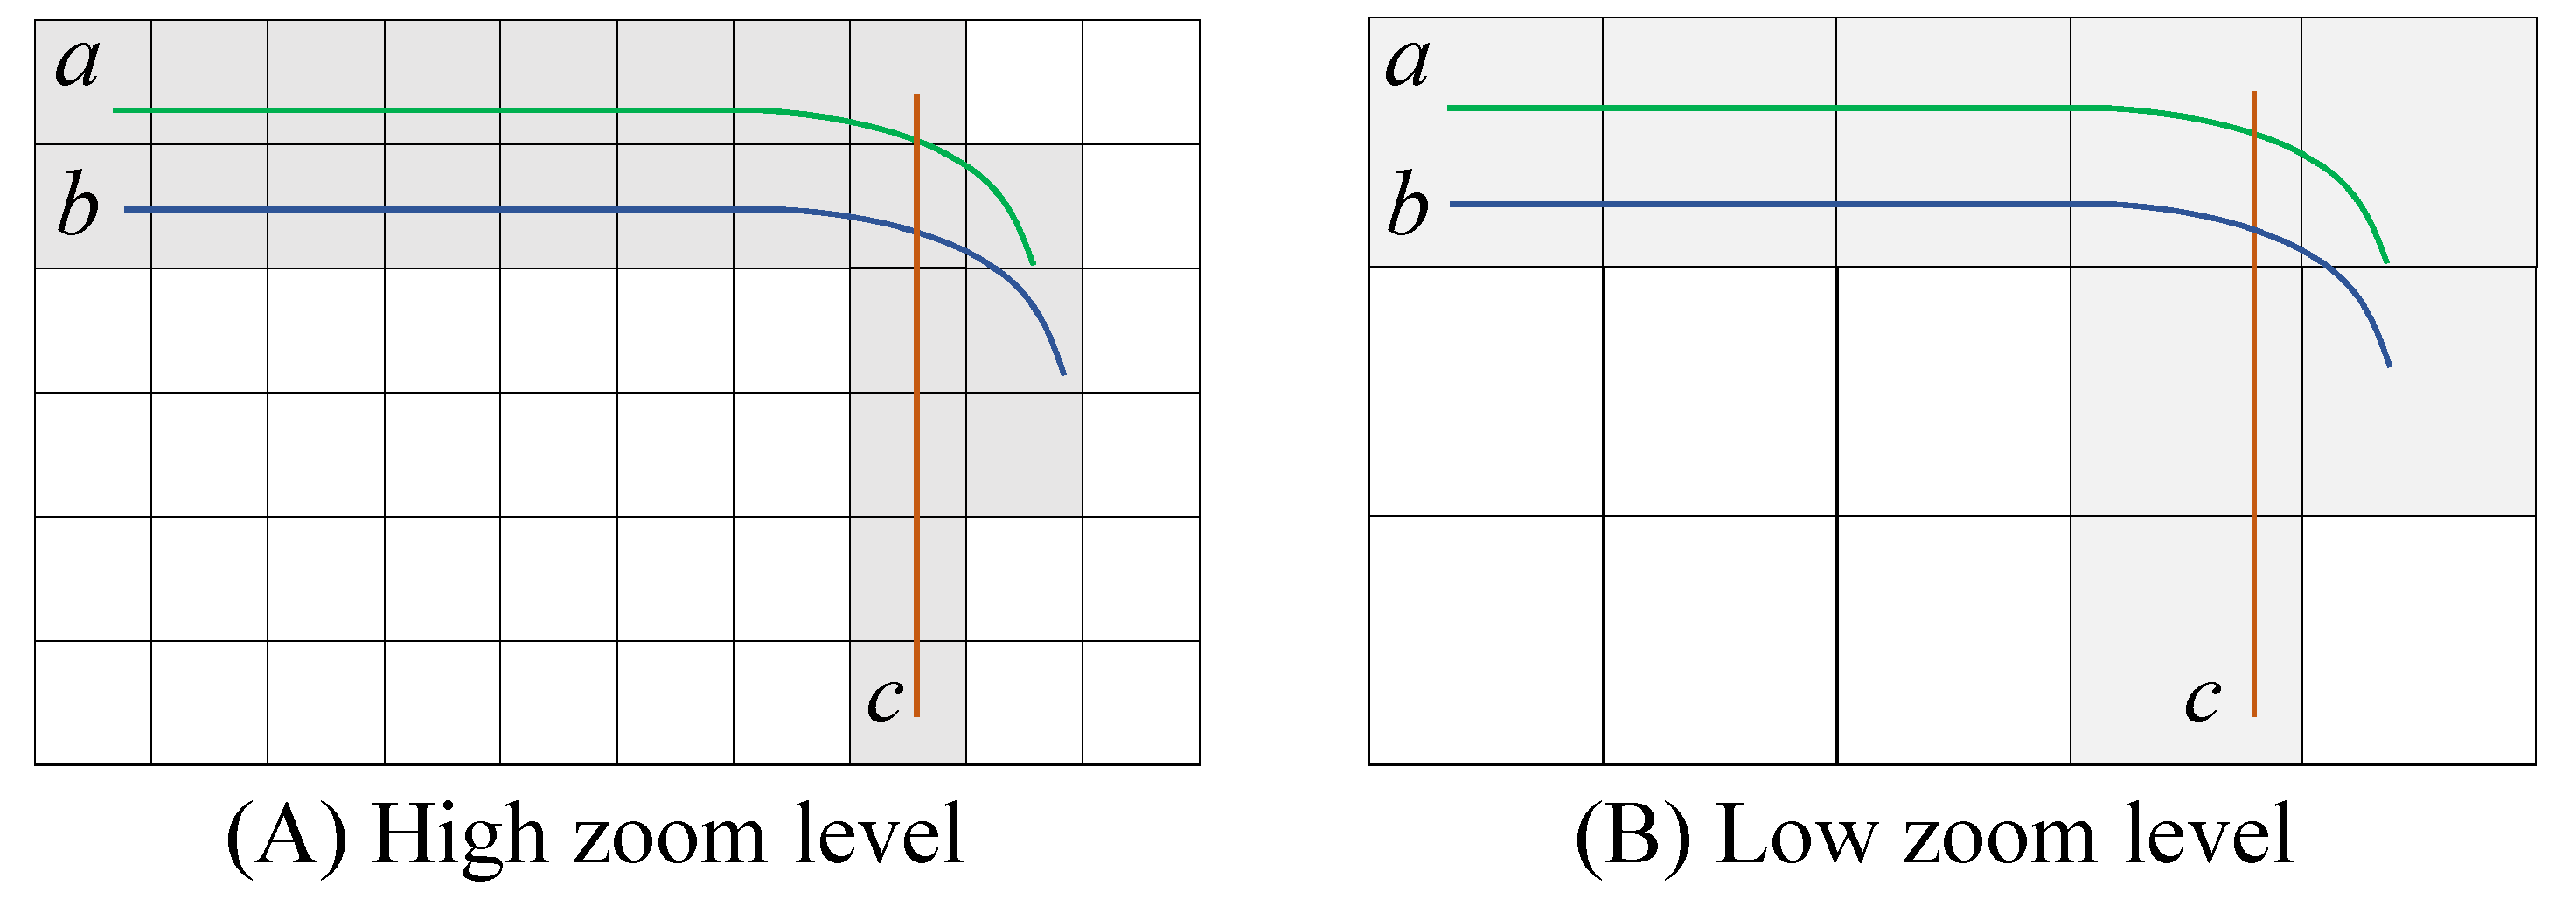
\includegraphics[width=0.4\textwidth]{pictures/problemsolveing/one_to_many.pdf}
%	\vspace{-5mm}
%	\caption{Resolution inconsistency}
%	\vspace{-5mm}
%	\label{fig:one_to_many}
%\end{figure}


%Specifically, $\avats$ incorporates a parameter $\delta$ during trajectory selection process in $\vats$ .
%In particular, we employ the parameter $\delta$ to model the end user's perception ability at the most high level of details.
%Surprisingly, our advance approach $\avats$ not only provides better visualization result when comparing with $\vats$ with the same sampling rate
%(e.g., Figure~\ref{fig:delta}(a) and (b) are the returning result of $\vats$ and $\avats$ respectively),
%but also embeds the popularity of selected trajectories by encoding the rest trajectories in the dataset in them,
%e.g., Figure~\ref{fig:delta}(c) is the visual result of $\avats$ with color encoded popularity.





\section{The $\avats$ Framework}\label{sec:cheetahtraj}
Recall that our goal is to provide high quality trajectory visualization for any user selected query region with low latency.
In this section, we first introduce the motivation behind the $\avats$ framework, then present its two key procedures: \textit{index building}, and \textit{query processing}.

\stitle{Motivation of $\avats$}
Given a user selected region query $\query$, a naive visualization procedure with our sampling algorithms works as follows:
it first retrieves all trajectories (or trajectory segments) that are in this region (a.k.a, $\wpts$ query~\cite{kruger2013trajectorylenses}),
then it invokes $\vatss$ (or $\vats$) to obtain a set $\oR$ of sample trajectories, and finally the trajectories in $\oR$ are rendered to the canvas (e.g., displaying device).
$\vatss$ has short \textit{visualization time} as it effectively reduces the number of processed locations by sampling. However, $\vatss$ has a long \textit{sampling time} (e.g., several seconds to tens of seconds) even with our performance optimization techniques.
Hence, the naive procedure can not achieve low latency for large-scale trajectory visualization. To tackle this problem, we propose the $\avats$ framework as illustrated in Figure~\ref{fig:framework}.  $\avats$ consists of three modules: (i) \textsf{index building}, (ii) \textsf{query processing}, and (iii) \textsf{result visualization}, we elaborate them as follows.


\begin{figure}
	\centering
	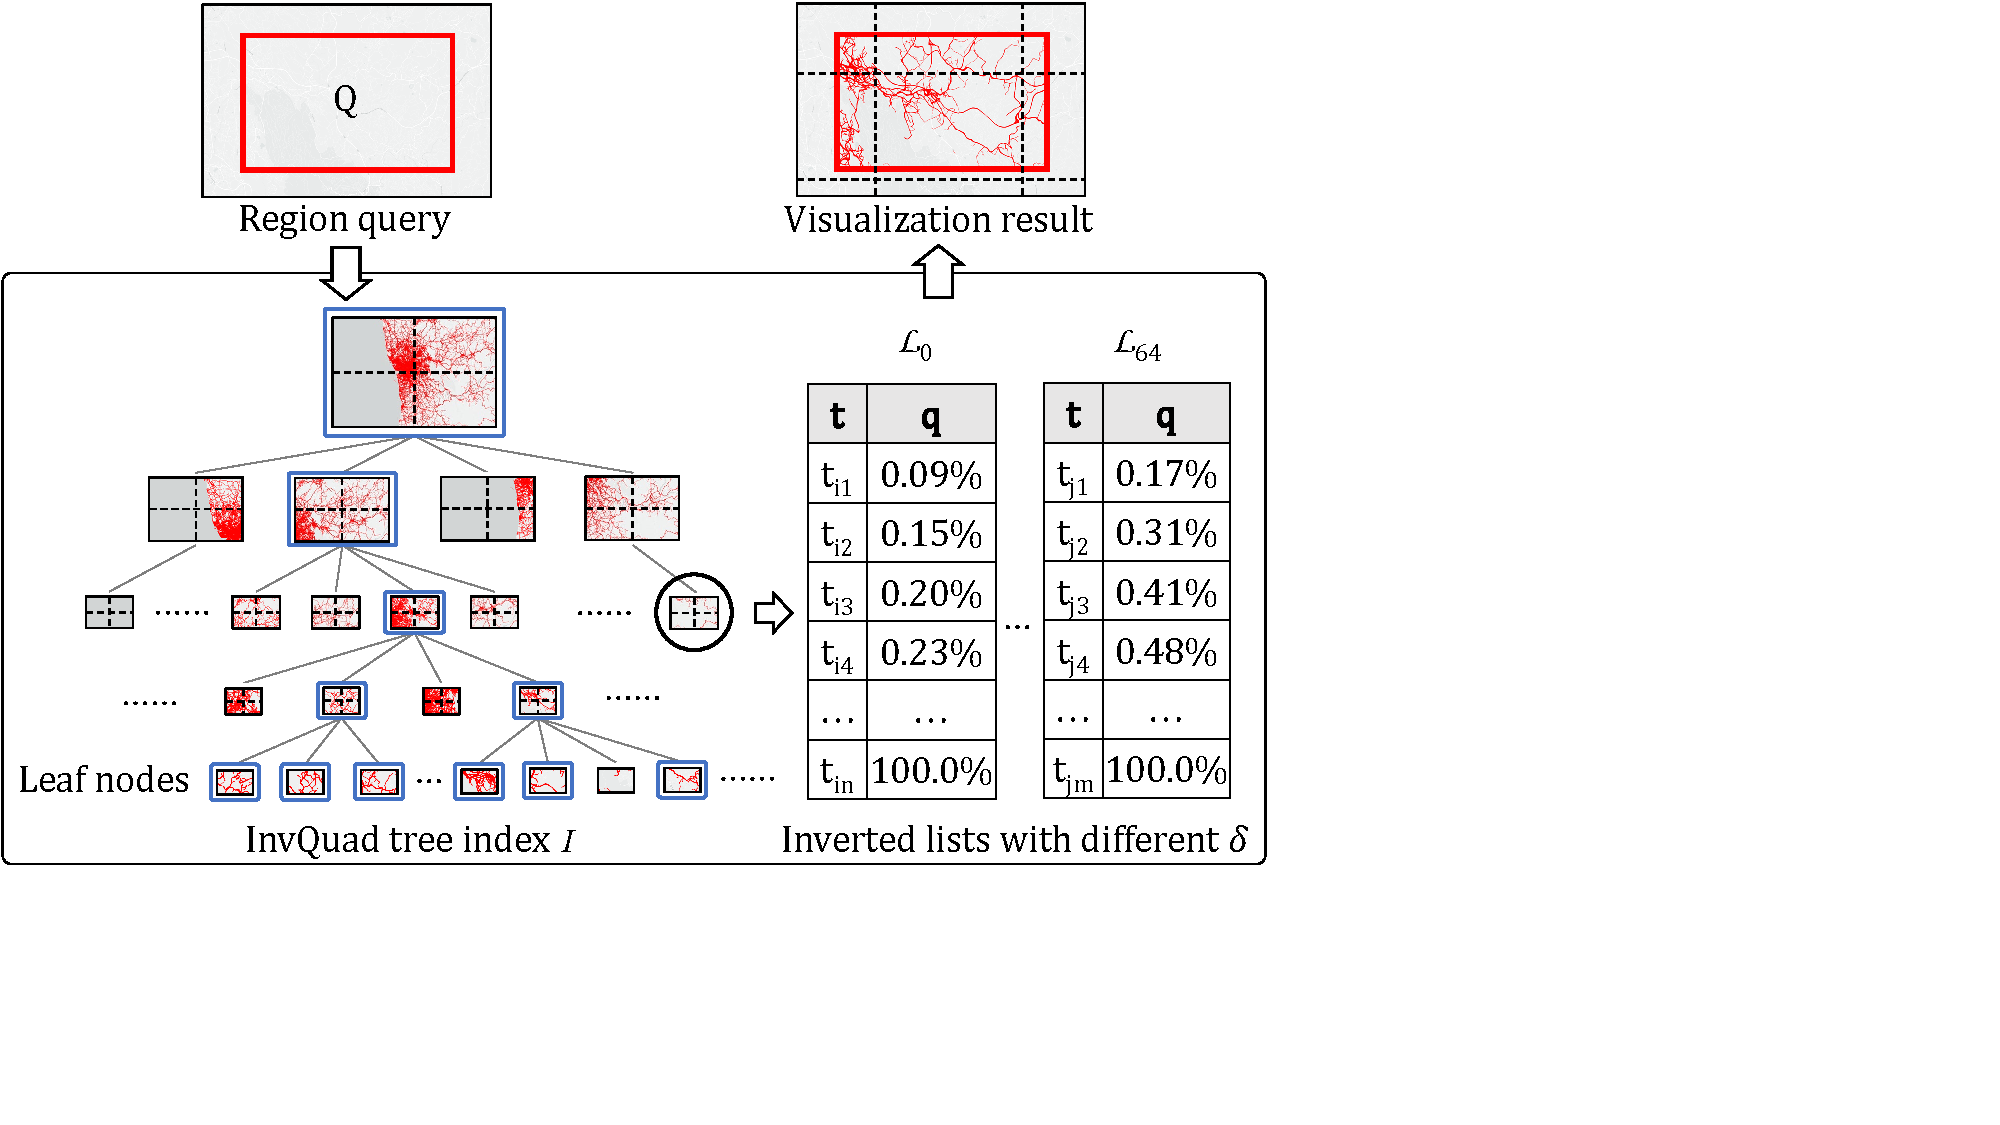
\includegraphics[width=0.4\textwidth]{pictures/cheetahtraj}
    \trim
    \caption{The $\avats$ framework}
    \label{fig:framework}
    \trim
\end{figure}


\subsection{Index Building}~\label{sec:index}
The key idea of $\avats$ is to conduct $\vatss$ sampling in the offline \emph{index building} phase such that the sampling results can be used for online visualization. To handle arbitrary query region, we develop an inverted list augmented quad-tree index ($\invQ$).

As shown in the example $\invQ$-tree index $\II$ at the bottom of Figure~\ref{fig:framework}, we exploit a quad-tree to recursively partition the entire area (spanned by the trajectory dataset) into smaller areas and manage each area with a tree node.
For each tree node, we run $\vatss$ using the trajectories (or trajectory segments) in its associated area as input to compute the \textit{visualization quality inverted lists} for this area. $\mathcal{L}_0$ and $\mathcal{L}_{64}$ in Figure~\ref{fig:framework} are two example visualization quality inverted lists, in which the subscripts are the values of $\delta$ for this list.
Specifically, we compute several inverted lists with different $\delta$ values\footnote{We set $\delta$ as 0 (i.e., $\vats$), 4, 8, 16, 32, 64. We need quality inverted lists with different $\delta$ for one area as the area may be covered by query regions of different sizes, and we use lists with larger $\delta$ for larger query region as discussed in Section~\ref{subsec:VQGS+}.} to support the efficient quality guaranteed result visualization at various zoom levels.
For each inverted list, (i) $\vatss$ terminates until the quality of the sample set is $100\%$, i.e., the visualization result of the sample set is the same as the full dataset;
(ii) the trajectory selected at each iteration of $\vatss$ is stored in the inverted list with its \textit{cumulative quality} in ascending order. Take inverted list $\mathcal{L}_0$ in Figure~\ref{fig:framework} for example, $t_{i4}$ is the trajectory selected at the $4$th iteration,
$t_{i4}$'s cumulative quality is $0.23\%$, which means that the quality achieved by $\{t_{i1}, t_{i2}, t_{i3}, t_{i4}\}$ as a whole is $0.23\%$. With the quality inverted list, searching a quality guaranteed sample set for a query region can be conducted efficiently via binary search.


\subsection{Query Processing}~\label{sec:query}
For a region visualization query $\query$ with quality threshold $\tau$, Algorithm~\ref{alg:query} summarizes the $\mathsf{Query}$ subroutine, which finds a quality guaranteed trajectory sample set $\oR$. The algorithm starts by invoking $\mathsf{Query}(\query, \tau, \II.root, \oR=\emptyset)$, i.e., from the root of $\invQ$-tree index $\II$ with an empty result set $\oR$, and then transverses the tree nodes recursively. If node   $\mathcal{N}$ is a leaf node or its associated area is entirely contained in the query region, we retrieve a quality guaranteed trajectory set by calling subroutine $\mathsf{findRet}()$, which conducts binary search on the proper inverted list in $\mathcal{N}$ (Line~\ref{line:ret}). Otherwise, we call $\mathsf{Query}()$ on the four children nodes of $\mathcal{N}$ ( Line~\ref{line:valls}-\ref{line:valle}). Note that Some trajectories in $\oR$, the result returned by $\mathsf{Query}()$ for region $\query$, may have segments outside $\mathcal{Q}$,
we conduct a way point query $\wpts(\query, \oR)$ to filter these segments before visualization.


\begin{algorithm}
	\caption{$\mathsf{Query}$($\query$, $\tau$, $\invQ$ node $\mathcal{N}$, result $\oR$)}
	\label{alg:query}
	\begin{algorithmic}[1]
        \If{ $\mathcal{N}$ is leaf node or  $\mathcal{N}$ is entirely contained in $\query$}
            \State $\oR \leftarrow \oR \cup \mathsf{findRet}(\mathcal{N}, \tau)$ \label{line:ret}
        \ElsIf {$\query \cap \mathcal{N} \neq \emptyset$} \label{line:valls}
            \For { $i$ from $0$ to $3$}
                \State $\mathsf{tmpQ} \leftarrow \query \cap \mathcal{N}.child[i]$
                \State $\mathsf{Query}(\mathsf{tmpQ}, \tau, \mathcal{N}.child[i], \oR)$
            \EndFor \label{line:valle}
        \EndIf
	\end{algorithmic}
\end{algorithm}


%

\stitle{Correctness analysis}
We first show that $\avats$ meets the visualization quality requirement in Theorem~\ref{theorem:quality} as follows.
\begin{theorem}\label{theorem:quality}
If all selected nodes in the $\invQ$-tree index $\II$ are entirely contained in the query region $\query$,
then the result set $\oR$ returned by Algorithm~\ref{alg:query} satisfies that $\QQ(\oR) \ge \tau$.
\end{theorem}
\begin{proof}
Suppose query region $\query$ selects areas $\mathcal{A}_1,\!\mathcal{A}_2,\!\cdots,\!\mathcal{A}_K$,
these areas satisfy $\mathcal{A}_i \cap \mathcal{A}_j = \emptyset$ for $i\neq j$, and $\cup_{k=1}^{K}\mathcal{A}_k=\mathcal{Q}$.
For each area $\mathcal{A}_k$, denote the number of points marked in the ground truth visualization as $n_k$,
and the number of points marked by the trajectories in $\mathcal{R}$ as $m_k$,
we have $\frac{m_k}{n_k} \ge \tau$ as we use the visualization quality inverted index for trajectory selection.
Thus, for query region $\query$ with result set $\oR$, we have
$\QQ(\oR) = \frac{\sum_{k=1}^{K} m_k}{\sum_{k=1}^{K} n_k} \ge \tau.$
\end{proof}
In more general cases, we also select some areas that only intersect with the query region $\query$ and the sample set $\oR$ may not satisfy $\frac{m_k}{n_k}\ge \tau$ for these areas.
This does not significantly affect visualization quality for two reasons:
(i) these areas are the leaf nodes of the $\invQ$-tree index and thus reside on the border of the query region.
When exploring the map, human tends to move the region of interest to the screen center, where is more ``close'' to eyes~\cite{fitts_click}. %fitts,
(ii) the areas of the border regions are small w.r.t. the query region if the $\invQ$-tree has a sufficient height (i.e., the leaf nodes have a small area).



\section{Experimental Evaluation}\label{sec:exp}

We first present a case study of the visualizations provided by $\avats$ in Section~\ref{sec:case} to demonstrate its good visualization quality. In Section~\ref{sec:user}, we conduct a comprehensive user study to compare the visualization quality of different methods. In Section~\ref{sec:quality}, we quantitatively compare the visual quality and efficiency of $\avats$ with the baselines.



%porto:总条数:2389863,总点数:75667503,最长:3490;  Shenzhen:总条数:3066861,总点数:53527890,最长:2268

\stitle{Experiment Settings} We use 3 real-world trajectory datasets, i.e., \pt{}, \sz{} and \cd{}, and their statistics are summarized in Table~\ref{tab:dataset}. The experiments are conducted on a machine with an Intel i7-8700 CPU, 24 GB memory and an NVIDIA GeForce GTX1080 GPU with 8 GB on-chip memory, running on Windows 10. All methods are implemented using Java 1.8. UnfoldingMap 0.9.92~\cite{ufmaps} is used to provide interactive map and GPS mapping, and the Processing 3 library~\cite{p3} is used for rendering. All timing results are measured in single-thread mode.

\begin{table}
	\centering
	\small
	\caption{Statistics of the datasets used in the experiments}
	\vspace{-3mm}
	\begin{tabular}{|c|c|c|c|c|} \hline
		Dataset & No. of Trajectories  & No. of GPS points  & Maximum length  \\ \hline
		\pt{}& 2,389,863 & 75,667,503 & 3,490 \\ \hline
		\sz{}& 3,066,861 & 53,527,890 & 2,268 \\ \hline
		\cd{}& 2,400,000 & 80,040,361 & 6,468 \\ \hline
	\end{tabular}	\label{tab:dataset}
	\vspace{-5mm}
\end{table}

%We conduct the experiments
%using 3 real-world trajectory datasets: \pt{}, \sz{} and \cd{}.
%\pt{}~\cite{pt} contains 2.39 million taxi trajectories and 75.67 million of GPS points, and the longest trajectory has 3,490 GPS points.
%\sz{}~\cite{sz} consists of 3.07 million taxi trajectories with 53.53 million GPS points, and the longest trajectory has 2,268 GPS points.
%\cd{}~\cite{cd} has 2.40 million taxi trajectories and 80.04 million GPS points, and the longest trajectory consists of 6,468 GPS points.  

%The datasets and source codes to reproduce our results are available at~\cite{code}.

\stitle{Baselines} We compare $\avats$ with three baselines, i.e., $\mathsf{Full}$, $\mathsf{Random}$ and $\mathsf{DTW}$. $\mathsf{Full}$ visualizes all trajectories in the user selected region while $\mathsf{Random}$ samples trajectories in the user selected region uniformly at random. $\mathsf{DTW}$ is based on the DTW distance between trajectories~\cite{borcan2012improving} and designed by us to select trajectories with good diversity. Specifically, $\mathsf{DTW}$ samples the trajectory that maximizes the aggregate DTW distance to all remaining trajectories in each step. It takes $\mathsf{DTW}$ several days to run on the experiment datasets because it needs to compute expensive DTW distance (quadratic complexity w.r.t. trajectory length) between all trajectory pairs. For fair comparison, we ensure that $\mathsf{Random}$ and $\mathsf{DTW}$ use the same number of trajectories as $\avats$.

\subsection{Case Study}\label{sec:case}

We conduct case study on the \pt{} dataset to demonstrate the visualization quality of $\avats$. The observations are similar for the other datasets and we omit their results for conciseness.

\begin{figure*}[t]
	\centering
	\includegraphics[width=0.85\textwidth]{pictures/case_study_icde/case_study_detail.pdf}
	\trim
	\vspace{-2mm}
	\caption{Case study of the visualization quality of $\avats$ for two detail regions.}
	\label{fig:detailview}
	\trim \trim
\end{figure*}

\begin{figure*}
	\centering
	\small
	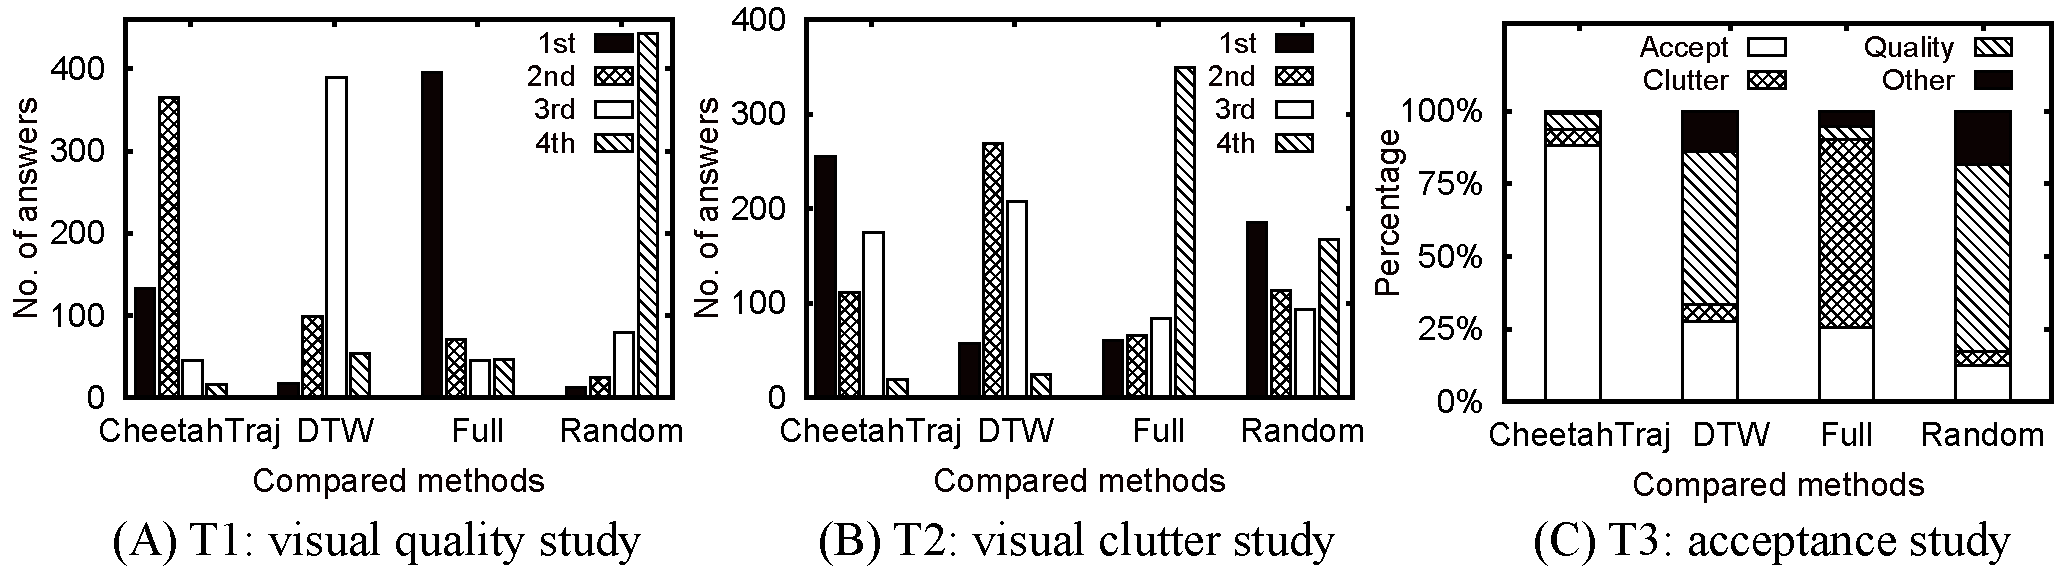
\includegraphics[width=1.3\columnwidth]{pictures/user_study/user_study.pdf}  
	\trim \trim
	%\vspace{-3mm}
	\caption{User study results of different visualization methods.} 
	\label{fig:userstudy}
	\trim \trim
\end{figure*}



\subsubsection{Overview visualization}

We illustrate the visualization results of different methods for the entire \pt{} dataset in Figure~\ref{fig:overview}.

\stitle{Good visual quality for overview}
At zoom level 11, Figure~\ref{fig:overview}(A) is the visualization result of $\mathsf{Full}$ on the \pt{} dataset.
With a sampling rate $\alpha \!=\! 1\%$, Figures~\ref{fig:overview}(B), (C) and (E) are the visualizations produced by $\mathsf{Random}$, $\mathsf{DTW}$,
and $\avats$, respectively. Comparing with Figure~\ref{fig:overview}(B) and (C), it is obvious that Figure~\ref{fig:overview}(E) is more similar to Figure~\ref{fig:overview}(A). In particular, Figure~\ref{fig:overview}(E) not only preserves the overall visual structure of the entire region but also keeps the details of cities that are far from the center (marked by the dashed cycles). However, the details of these cities are lost in Figure~\ref{fig:overview}(B) as $\mathsf{Random}$ mostly selects trajectories in the dense region. $\mathsf{DTW}$ in Figure~\ref{fig:overview}(C) preserves more details than $\mathsf{Random}$ in the sparse regions as it considers diversity in trajectories but its visualization quality is still inferior compared with $\avats$ in Figure~\ref{fig:overview}(E).

\stitle{Good visual quality under different sampling rates}
Figure~\ref{fig:overview}(D) and (E) are the visualizations produced by $\avats{}$ with a sampling rate of $0.1\%$ and $1\%$, respectively. We can make two observations: (i) the larger the sampling rate, the better the visual quality, i.e., Figures~\ref{fig:overview}(E) is more similar to Figure~\ref{fig:overview}(A) than Figure~\ref{fig:overview} (D); (ii) the visualization of $\avats$ with a sampling rate of $0.1\%$ (i.e., Figure~\ref{fig:overview}(D)) looks more appealing than the visualizations of $\mathsf{Random}$ and $\mathsf{DTW}$ with a sampling rate of $1\%$ (i.e., Figure~\ref{fig:overview}(B) and (C)) as Figure~\ref{fig:overview}(D) better preserves the structures in Figure~\ref{fig:overview}(A).



\stitle{Color encoding effectively mitigates visual clutter} At zoom level 11 and with a sampling rate of $1\%$, Figures~\ref{fig:overview}(E) and (F) are the visualizations produced by our $\avats$ and $\cavats$ (i.e., enabling color encoding), respectively.
Visual clutter is severe for $\mathsf{Full}$ (i.e., Figure~\ref{fig:overview}(A)) and $\avats$ (i.e., Figure~\ref{fig:overview}(E)) as many pixels are visualized for the dense region in the center, which makes it difficult to identify the main routes. The visualization of $\cavats$ in Figure~\ref{fig:overview}(F) alleviates this problem by encoding more representative trajectories with warmer color, making it easier to identify some main routes than Figure~\ref{fig:overview}(A) and (E).

%\vspace{1mm}
\subsubsection{Detail visualization}\label{sec:detail}




We analyze the visualizations produced by different methods for small areas with details by investigating two regions of interest in the \pt{} dataset in Figure~\ref{fig:detailview}.

%We next present the effectiveness of our proposals with detail views by investigating two regions of interest in \pt{}, the dense region B and the sparse region C(shown as in Figure~\ref{fig:detailview}(8)).

%$\mathsf{Full}$
%$\mathsf{DTW}$
%$\mathsf{Random}$

\stitle{Reduce visual clutter and preserve micro structures for dense region} At zoom level 15, region B in Figure~\ref{fig:detailview}(A) is the center of Porto and has the highest concentration of trajectories. Therefore, $\mathsf{Full}$ suffers from severe visual clutter and it is difficult to identify the road networks in Figure~\ref{fig:detailview}(B1).  $\mathsf{Random}$ and $\mathsf{DTW}$ in Figure~\ref{fig:detailview}(B2) and (B3) reduce the visual clutter to some extent by sampling some trajectories. $\avats$ in Figure~\ref{fig:detailview}(B4) is more successful in reducing the visual clutter of $\mathsf{Full}$ and allows to identify a much larger number of routes. In addition, $\avats$ preserves more micro structures of the trajectories than $\mathsf{Random}$ and $\mathsf{DTW}$, e.g., the circular route in the dashed circular region.

% and causes serious visual clutter, as visualized in Figure~\ref{fig:detailview}(B1).
%For example, the circular structures of the main route(shown as the dashed circular region in Figure~\ref{fig:detailview}(B1)) is unclear.
%$\localavats$ alleviates the visual clutter by preserve the $1\%$ trajectories of the total regions but the clutter is still serious. Furthermore, $\avats$ performs better than $\localavats$ by preserving less trajectories and reduce the visual clutter.


\stitle{Preserve overall layout for sparse region}
At zoom level 14, region C in Figure~\ref{fig:detailview}(A) contains the city of Casino Espinho and has fewer trajectories than the dense region in the center. In this case, the sampling methods need to keep the overall layout of the trajectories  to provide good visualization quality. Compared with $\mathsf{Full}$ in Figure~\ref{fig:detailview}(C1), $\mathsf{Random}$ and $\mathsf{DTW}$ in Figure~\ref{fig:detailview}(C2) and (C3) fail to meet this requirement as they do not show any trajectory for areas far from the city, e.g., in the dashed circle. This makes their entire visualization layout very different from $\mathsf{Full}$. In contrast, $\avats$ in Figure~\ref{fig:detailview}(C4) preserves the trajectories in areas far from the city and has a overall layout similar to $\mathsf{Full}$.

%Region C includes the city of Casino Espinho at zoom level 14, which contains less trajectories than the center of Porto as the visualization result of full dataset shown in Figure~\ref{fig:detailview}(C1).
%Given fix sampling rate $\alpha=1\%$, Figure~\ref{fig:detailview}(C2) indicates the visualization of $\localavats$. This visualization result misses a lot if detail information in this region, because the fix sampling rate preserves too few trajectories which is difficult to guarantee the visual quality.
%While $\avats$ in Figure~\ref{fig:detailview}(C3) performs much better than $\localavats$ as the sampling rate is automatically adjusted to according to the visual quality. In this visualization, the trajectory sketch of Casino Espinho is almost the same as it in Figure~\ref{fig:detailview}(C1), the visualized result of full dataset.

%To sum up, the case study shows that $\avats$ effectively mitigates visual clutter with sampling and color encoding. With the quality-aware $\vatss$ algorithm, $\avats$ also provides better visualization quality than $\mathsf{Random}$ and $\mathsf{DTW}$ by preserving the micro structures and overall layout of full visualization.

To sum up, the case study shows that $\avats$ effectively mitigates visual clutter. In addition, $\avats$ also provides better visualization quality than $\mathsf{Random}$ and $\mathsf{DTW}$ by preserving the micro structures and overall layout of full visualization.

\subsection{User Study}\label{sec:user}


\if 0
\begin{figure*}
     \centering
     \begin{tabular}{ccc}
		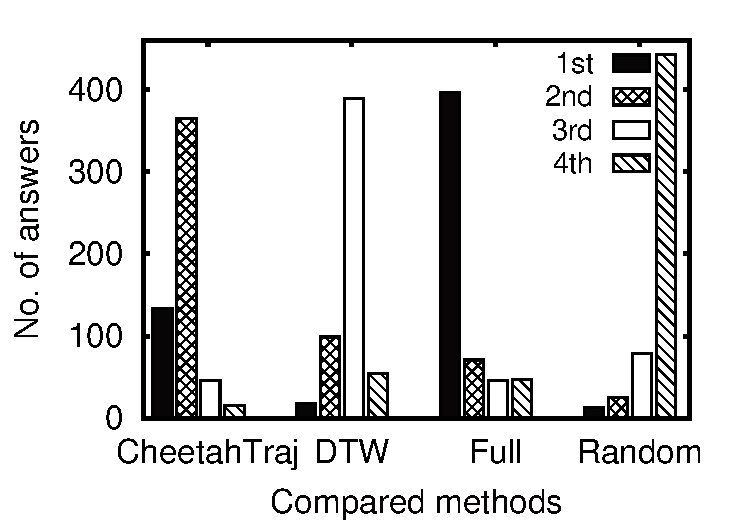
\includegraphics[width=0.22\linewidth]{pictures/user_study/quality}
		&
		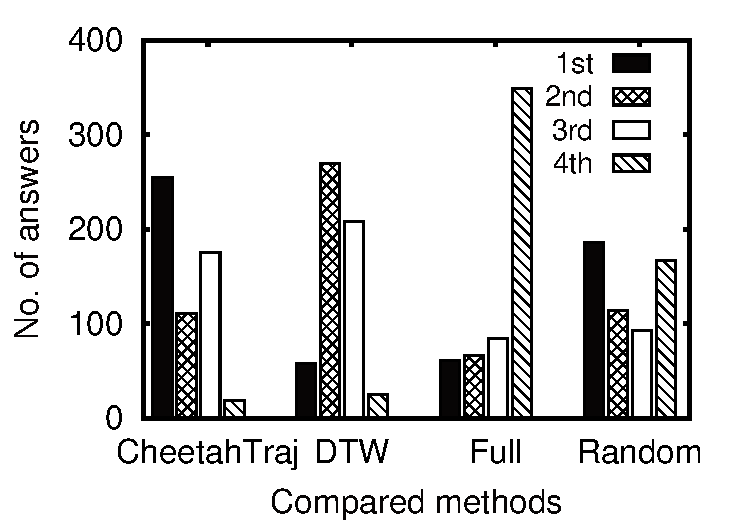
\includegraphics[width=0.22\linewidth]{pictures/user_study/clutter}
        &
        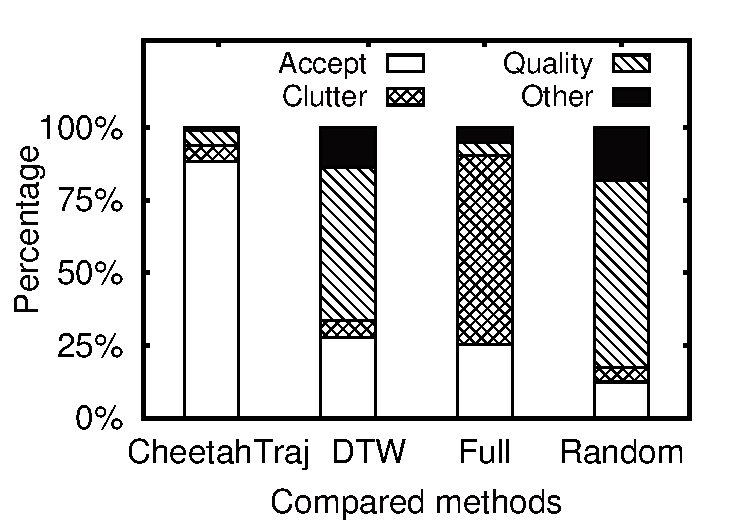
\includegraphics[width=0.22\linewidth]{pictures/user_study/accept}
		\\
		(A) T1: visual quality study
		&
		(B) T2: visual clutter study
        &
        (C) T3: acceptable visualization study
	\end{tabular}
	\vspace{-4mm}
	\caption{User study results of different visualization methods}
	\label{fig:userstudy}
    \trim
\end{figure*}
\fi

In this part, we conduct a user study to evaluate the quality of the visualizations generated by different methods objectively.


%We recruited 35 participants with 10 females, 25 males, aged 19 to 31 with a mean of 24.78 for the user study. 
%The user study is conducted on the \pt{} and \sz{} datasets, and four visualization methods are investigated, i.e., $\full$, $\rand$, $\mathsf{DTW}$ and $\avats$. 
%We manually select 22 \textit{center points} in the two datasets and define 3 \textit{visualization scales} including: large-scale region (with zoom level smaller than 13), middle-scale region (with zoom level between 13 and 15), small-scale region (with zoom level larger than 15). For each center point and at each visualization scale, we generate a \textit{comparable visualization group}, which includes one visualization generated by each of the 4 methods. This results in 66 comparable groups (22 center points $\times$ 3 scales) and 264 visualization results (66 comparable groups $\times$ 4 visualizations).

\stitle{Settings} We recruited 35 participants with 10 females, 25 males, aged 19 to 31 with a mean of 24.78 for the user study. The user study is conducted on the \pt{} and \sz{} datasets, and four visualization methods are investigated, i.e., $\full$, $\rand$, $\mathsf{DTW}$ and $\avats$. We define a \textit{comparable group} as the set of visualizations generated by different methods with the same center point and zoom scale. We manually generated 66 comparable groups and 264 visualizations results (66 groups $\times$ 4 visualizations). The user study system is a web-based platform, in which all visualizations are displayed with a resolution of 450*300. We are interested in the visual quality and visual clutter of the visualizations, and thus designed three tasks for a comparable group:
\begin{itemize}
	\item Task 1 (T1): rank the visualizations in a group from the highest visual quality to the lowest visual quality. %by 1st, 2nd, 3rd, and 4th.
	\item Task 2 (T2): rank the visualizations in a group from the least visual clutter to the most severe visual clutter. %by 1st, 2nd, 3rd, and 4th.
	\item Task 3 (T3): select the visualizations considered acceptable (multiple choices allowed) and choose the reason (including ``severe visual clutter", ``poor visual quality" and ``others") for the visualizations considered unacceptable. 
\end{itemize}


\stitle{User study procedure} 
When the participants enter the user study system, they are given a tutorial on how to conduct the tasks to get familiar with the interface and tasks.
For each participant, we randomly select 16 comparable groups.
%Thus, we obtain $35 \times 16 = 560$ results for each task.
For each comparable group, the 4 visualizations (\textit{without specifying generated by which method}) in it are displayed on the same page and a participant is required to perform task T1, T2 and T3 by inspecting them.


%The results show that $\full$ ranks the 1st in most cases while $\avats$ usually ranks 1st or 2nd. i.e., the percentage of $\avats$ ranks top-2 among 4 methods is $88.9\%$. 
%In contrast, $\mathsf{DTW}$ and $\rand$ rank 3rd and 4th at most times. 
%This suggests that the visualizations generated by $\avats$ are more appealing to the participants than $\mathsf{DTW}$ and $\rand$. 
%We also observed that the participants tend to rank $\avats$ before $\full$ for large-scale regions with  many trajectories, and the other way for smaller regions. 
\stitle{Result analysis} 
Figure~\ref{fig:userstudy}(A) reports the visual quality ranking of the 4 methods in T1. The results show that $\full$ ranks 1st in most cases while $\avats$ usually ranks 1st or 2nd. 
In contrast, $\mathsf{DTW}$ and $\rand$ rank 3rd and 4th at most times. 
This suggests that the visualizations generated by $\avats$ are more appealing to the participants than $\mathsf{DTW}$ and $\rand$. Figure~\ref{fig:userstudy}(B) reports the anti-visual clutter ranking of the 4 methods in T2. 
The results show that visual clutter is most severe for $\full$, ranking 4th in most cases.    
While $\avats$ is the most successful in reducing visual clutter, ranking 1st in 255 out of the 560 cases and ranking 4th for only 19 cases.
We report the acceptance frequency of the 4 methods in T3 using bar chart in Figure~\ref{fig:userstudy}(C). 
Each column corresponds to a method, and from bottom to top, the lengths of the bars indicate the percentage of participants choosing ``acceptable'', ``not acceptable due to visual clutter'', ``not acceptable due to poor visual quality'' and ``not acceptable for other reasons''. 
The results show that $\avats$ is regarded acceptable for about 88.2\% of the cases, and the other methods have much lower acceptance rate than $\avats$.   

%The time usage for T1 range from 816  seconds to 5748 seconds with a mean of 2320 seconds.
%We also observed that the participants tend to rank $\avats$ before $\full$ for large-scale regions with  many trajectories, and the other way for smaller regions. 

%Figure~\ref{fig:userstudy}(B) reports the anti-visual clutter ranking of the 4 methods in T2. 
%The results show that visual clutter is most severe for $\full$, ranking 4th in most cases (349 over 560). With sampling, $\mathsf{DTW}$ usually rank 2nd and 3rd but $\rand$ ranks 4th for a considerable number of times as it tends to create clutter in the dense regions.    
%$\avats$ is the most successful in reducing visual clutter, ranking 1st in 255 out of the 560 cases and ranking 4th for only 19 cases.    

%\QM{Figure~\ref{fig:userstudy}(B) reports the anti-visual clutter ranking of the 4 methods in T2. 
	%The results show that visual clutter is most severe for $\full$, ranking 4th in most cases.    
	%While $\avats$ is the most successful in reducing visual clutter, ranking 1st in 255 out of the 560 cases and ranking 4th for only 19 cases. 
	%The time usage for T2 range from 513 seconds to 9503 seconds with a mean of 2320 seconds.}

%We report the frequency each of the 4 methods is selected as acceptable and why a method is not selected in T3 using bar chart in Figure~\ref{fig:userstudy}(C). 
%Each column corresponds to a method, and from bottom to top, the lengths of the bars indicate the percentage of participants choosing ``acceptable'', ``not acceptable due to visual clutter'', ``not acceptable due to poor visual quality'' and ``not acceptable for other reasons''. 
%The results show that $\avats$ is regarded acceptable for about 88.2\% of the cases, and the other methods have significantly lower acceptance rate than $\avats$. 
%Specifically, $\mathsf{DTW}$ and $\rand$ have low acceptance rate mainly due to poor visual quality while $\full$ suffers from severe visual clutter.

%\QM{We report the acceptance frequency of the 4 methods in T3 using bar chart in Figure~\ref{fig:userstudy}(C). 
	%Each column corresponds to a method, and from bottom to top, the lengths of the bars indicate the percentage of participants choosing ``acceptable'', ``not acceptable due to visual clutter'', ``not acceptable due to poor visual quality'' and ``not acceptable for other reasons''. 
	%The results show that $\avats$ is regarded acceptable for about 88.2\% of the cases, and the other methods have significantly lower acceptance rate than $\avats$. The time usage for T3 range from 539 seconds to 1334 seconds with a mean of 1018 seconds.
	%Specifically, $\mathsf{DTW}$ and $\rand$ have low acceptance rate mainly due to poor visual quality while $\full$ suffers from severe visual clutter.
%}




\begin{figure*}
	\centering
	\small
	\begin{tabular}{ccc}
		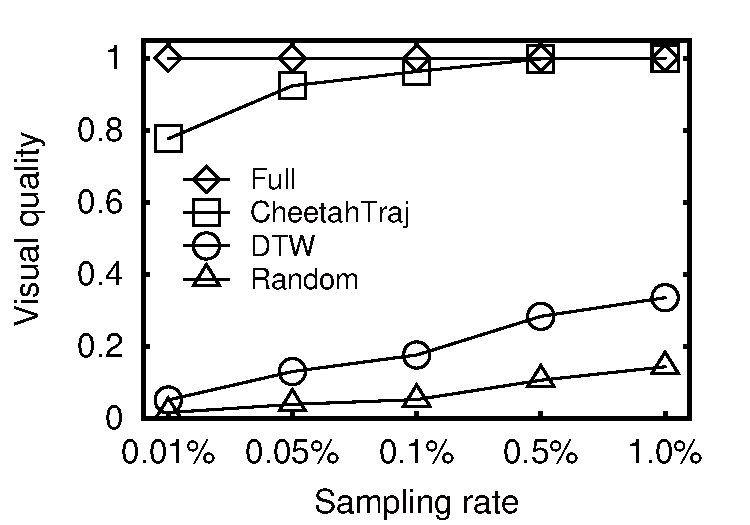
\includegraphics[width=0.28\linewidth]{pictures/quantitative_study/rate_porto_q}
		&
		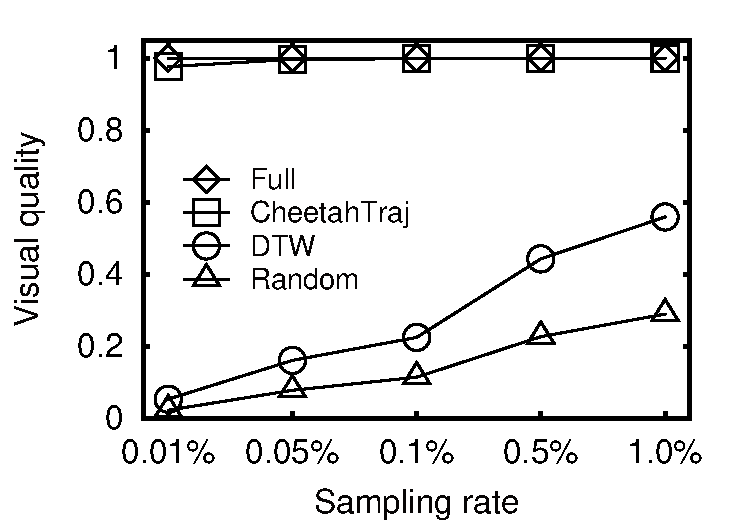
\includegraphics[width=0.28\linewidth]{pictures/quantitative_study/rate_sz_q}
        &
		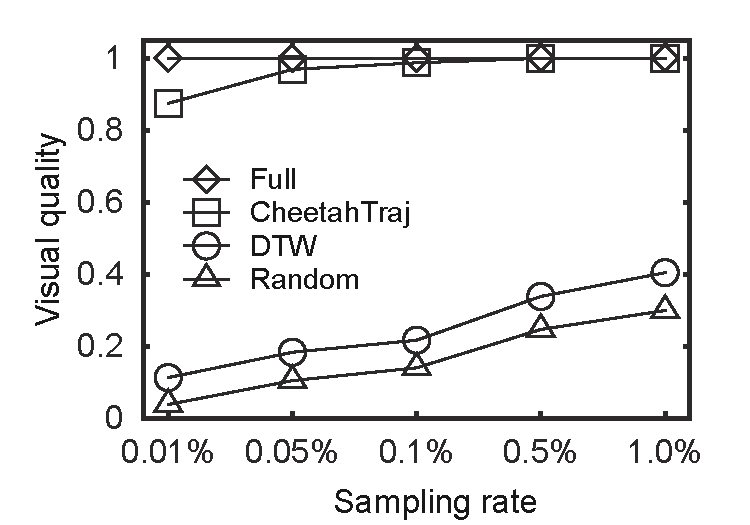
\includegraphics[width=0.28\linewidth]{pictures/quantitative_study/rate_cd_q}
		\\
		(A) \pt{}
		&
		(B) \sz{}
		&
		(C) \cd{}
	\end{tabular}
    \trim
	\caption{Effect of varying sampling rate visual quality.}
	\label{fig:rate_quality}
	\trim \trim
\end{figure*}

\begin{figure*}
	\centering
	\small
	\begin{tabular}{ccc}
		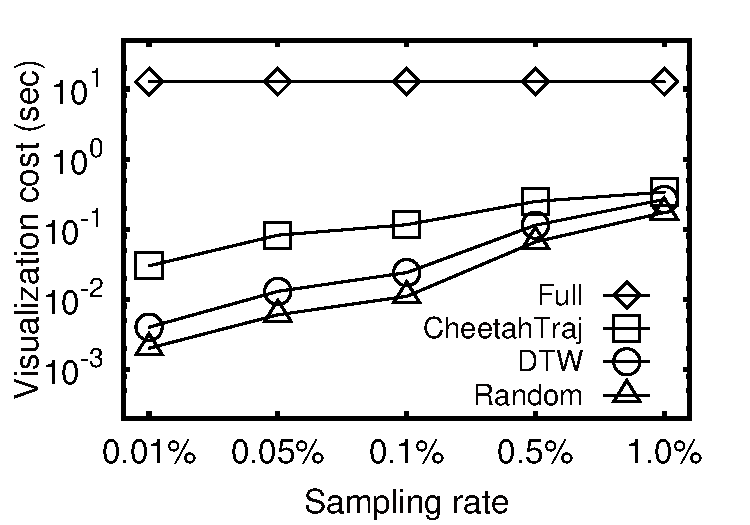
\includegraphics[width=0.28\linewidth]{pictures/quantitative_study/rate_porto_t}
		&
		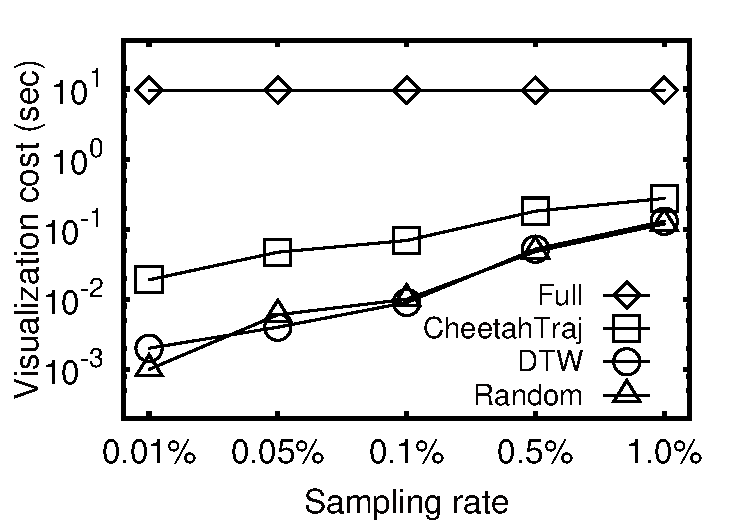
\includegraphics[width=0.28\linewidth]{pictures/quantitative_study/rate_sz_t}
        &
		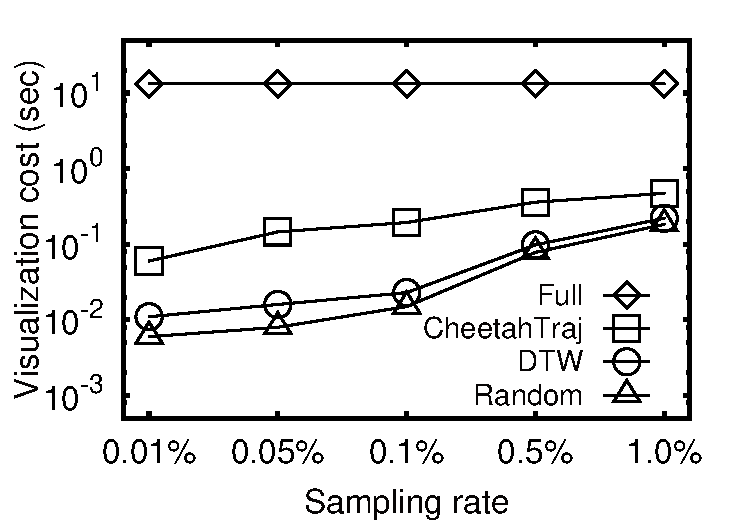
\includegraphics[width=0.28\linewidth]{pictures/quantitative_study/rate_cd_t}
		\\
		(A) \pt{}
		&
		(B) \sz{}
		&
		(C) \cd{}
	\end{tabular}
    \trim
	\caption{Effect of  sampling rate on visualization cost.}
	\label{fig:rate_vistime}
	\trim \trim
\end{figure*}

\begin{figure*}
	\centering
	\small
	\begin{tabular}{ccc}
		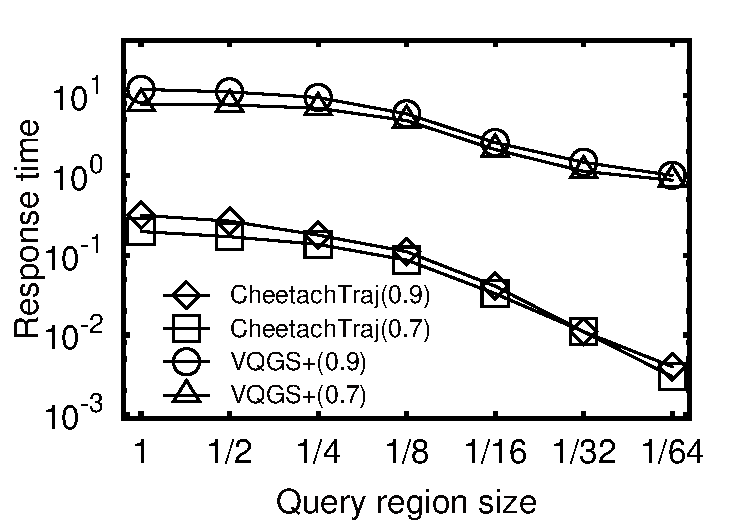
\includegraphics[width=0.28\linewidth]{pictures/quantitative_study/size_porto_t}
		&
		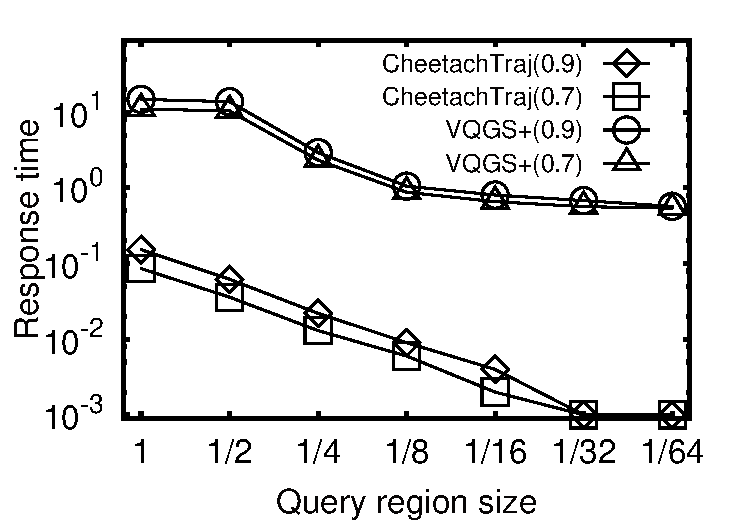
\includegraphics[width=0.28\linewidth]{pictures/quantitative_study/size_sz_t}
		&
		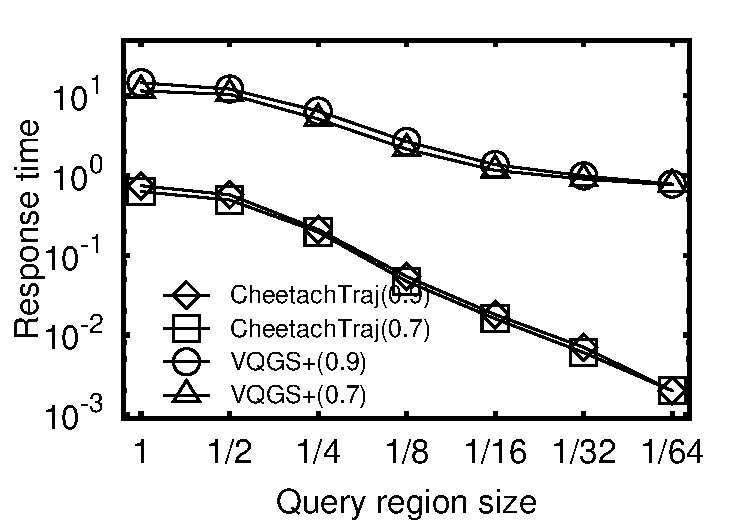
\includegraphics[width=0.28\linewidth]{pictures/quantitative_study/size_cd_t}
		\\
		(A) \pt{}
		&
		(B) \sz{}
		&
		(C) \cd{}
	\end{tabular}
    \trim
	\caption{Effect of region size on end-top-end response time.}
	\label{fig:size_responsetime}
	\trim \trim
\end{figure*}


\begin{figure*}
	\centering
	\small
	\begin{tabular}{ccc}
		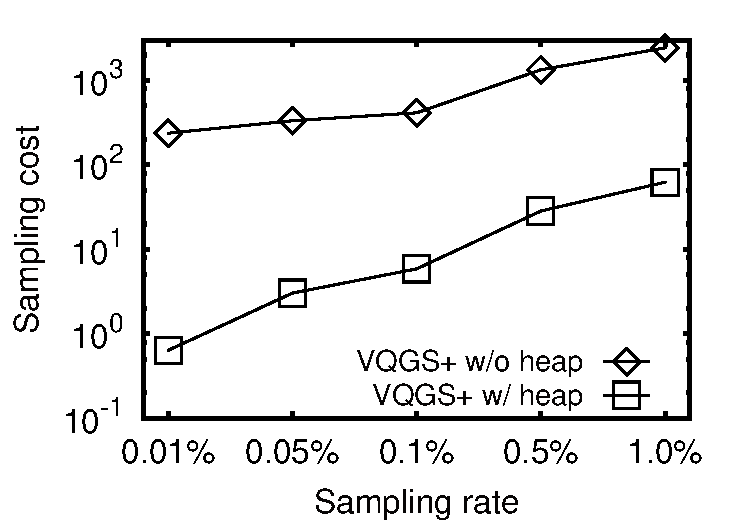
\includegraphics[width=0.28\linewidth]{pictures/quantitative_study/vqgs_porto_t}
		&
		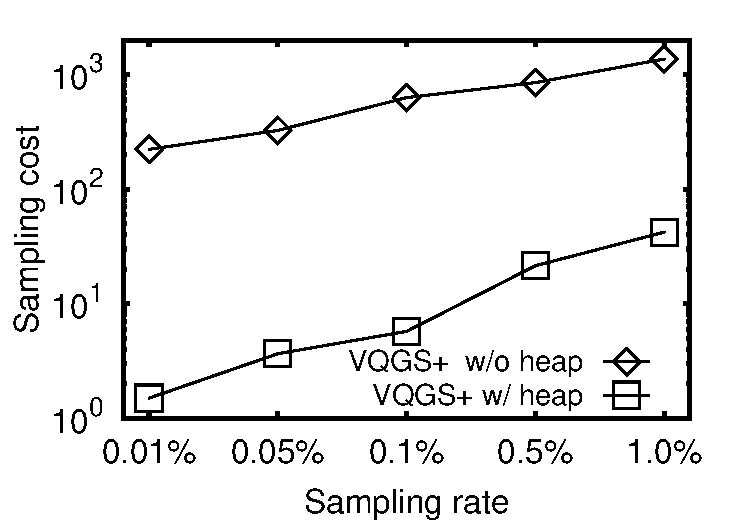
\includegraphics[width=0.28\linewidth]{pictures/quantitative_study/vqgs_sz_t}
		&
		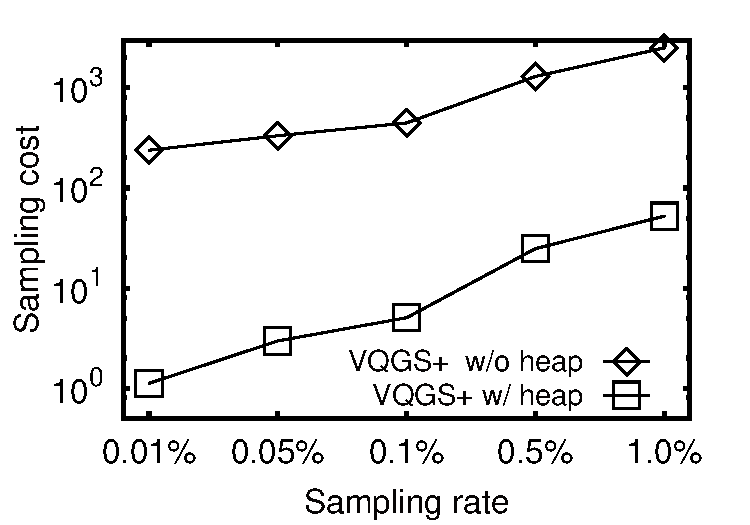
\includegraphics[width=0.28\linewidth]{pictures/quantitative_study/vqgs_cd_t}
		\\
		(A) \pt{}
		&
		(B) \sz{}
		&
		(C) \cd{}
	\end{tabular}
    \trim
	\caption{Effect of sampling rate on the sampling cost of $\vatss$ with/without optimization}
	\label{fig:rate_algtime}
	\trim \trim
\end{figure*}

\subsection{Quantitative Evaluation}\label{sec:quality}
In this part, we quantitatively evaluate the visual quality and efficiency of $\avats$ on the three real-world trajectory datasets.

\stitle{Visual quality} Figure~\ref{fig:rate_quality} reports the visualization quality (as defined in Equation~\eqref{eqref:loss}) of the methods under different sampling rate.
We consider the entire region in each dataset for this experiment.
The results show that our proposal $\avats$ achieves significantly higher quality than $\rand$ and $\mathsf{DTW}$ under the same sampling rate.
This is because the sampling algorithm $\vats$ and $\vatss$ in the $\avats$ framework are designed with explicit considerations for visual quality.
Specifically, the quality of $\avats$ approaches 1 when the sampling rate is still less than 1\% for all 3 datasets.
$\mathsf{DTW}$ has a higher quality than $\rand$ because it considers the diversity of trajectories.


In Figure~\ref{fig:rate_vistime}, we report the visualization cost (i.e., the wall clock time to generate visualization result using the sampled trajectories) for the methods under different sampling rate.
We still consider the entire region in this experiment and the visualization time of $\full$ (which does not change with sampling rate) is included at the top of each figure for reference.
The results show that all sampling methods achieve significantly shorter visualization cost than $\full$, and the speedup can be 1 to 4 orders of magnitude.
This confirms our observation that sampling is effective in improving visualization efficiency.
Under the same sampling rate, our $\avats$ takes slightly longer visualization time than $\rand$ and $\mathsf{DTW}$
because $\avats$ tends to select long trajectories for quality maximization.
%It is worth to point out the largest visualization cost of $\avats$ in \pt{}, \sz{} and \cd{} are 0.339, 0.275 and 0.471
Combining Figure~\ref{fig:rate_quality} and~\ref{fig:rate_vistime}, we can conclude that $\avats$ can achieve high visualization quality with  short visualization latency.


\stitle{Efficiency of $\avats$}
We evaluate the \textit{response time} of our $\avats$ framework under different quality guarantees and region sizes in Figure~\ref{fig:size_responsetime}.
The response time of $\avats$ is the end-to-end time for generating visualization for a selected region, which includes querying the $\avats$ index and computing the visualization.
For comparison, we also plot the response time of $\vatss$ (with $\delta\!=\!8$), which uses on-line sampling instead of querying the index in $\avats$ framework.
We constrain the regions to be rectangles with a constant height/width ratio and measure the size of a region by dividing its height over the height of the entire region.
For each region size, we report the average response time of three typical regions, i.e., a dense region, a sparse region and a medium region.
The results show that $\avats$ achieves a short response time (less than 1 second in all cases and 0.2 second for most cases) for different region sizes and quality guarantees. $\vatss$ is 1 to 2 orders of magnitude slower than $\avats$ and takes at most 14.802 seconds in all cases. These results show that $\vatss$ cannot support interactive visual exploration and the $\invQ$-tree index in $\avats$ is effective in improving efficiency.
In addition, the response time decreases rapidly when the region size shrinks as there are fewer trajectories in a smaller region.
However, the response time required to achieve a high quality (e.g., 0.9) is not significantly longer than a low quality (e.g., 0.7) as quality improves quickly with the number of sampled trajectories as a shown in Figure~\ref{fig:rate_quality}.





\stitle{Effect of heap-based lazy computation}
In Figure~\ref{fig:rate_algtime}, we report the running time of $\vatss$  with and without the heap-based lazy computation.
The results show that the heap-based optimization reduces the running time of $\vatss$ around 2 orders of magnitude.
For the sampling rates we considered, $\vatss$ runs efficiently and can finish within 1 second for the entire dataset.



%\begin{figure}[t]
%	\centering
%	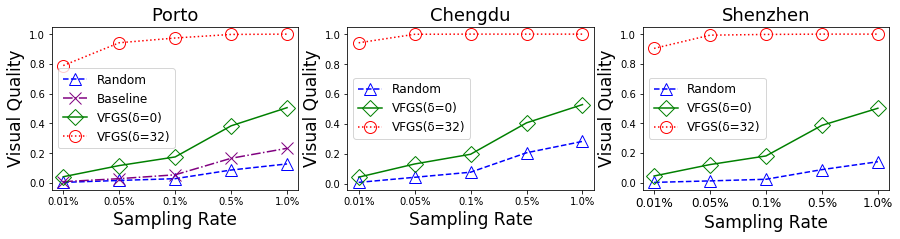
\includegraphics[width=0.5\textwidth]{pictures/quantitative_study_icde/sample_quality.png}
%	\vspace{-8mm}
%	\caption{Visual quality vs. sampling rates.}
%	\label{fig:sample_quality}
%	\vspace{-3mm}
%\end{figure}

%\begin{figure}[t]
%	\centering
%	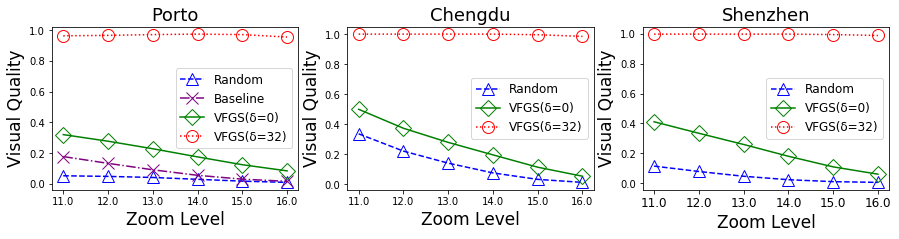
\includegraphics[width=0.5\textwidth]{pictures/quantitative_study_icde/zoom_quality.png}
%	\vspace{-8mm}
%	\caption{Visual quality vs. zoom level.}
%	\label{fig:zoom_quality}
%	\vspace{-3mm}
%\end{figure}


%\begin{table}
%	\centering
%	\small
%	\caption{The cost of $\invQ$-tree index}
%	\begin{tabular}{|@{}c@{}|@{}c@{}|@{}c@{}|@{}c@{}|@{}c@{}|} \hline
%		Dataset (size) & Height & Building time & Memory size \\ \hline
%		\pt{} (1.44G)	& 13 & 526.390s & 3.65GB  \\ \hline
%		\sz{} (1.02G)	& 13 & 435.291s  & 3.12GB \\ \hline
%		\cd{} (1.49G)	& 13 & 454.151s & 3.71GB \\ \hline
%	\end{tabular}	\label{tab:index cost}
%    \trim %\trim
%\end{table}

\begin{table}
	\centering
	\small
	\caption{The cost of $\invQ$-tree index}
	\begin{tabular}{|c|c|c|c|} \hline
		Dataset (size) & Height & Building time & Memory size \\ \hline
		\pt{} (1.44G)	& 13 & 526.390s & 3.65GB  \\ \hline
		\sz{} (1.02G)	& 13 & 435.291s  & 3.12GB \\ \hline
		\cd{} (1.49G)	& 13 & 454.151s & 3.71GB \\ \hline
	\end{tabular}	\label{tab:index cost}
	\trim %\trim
\end{table}

\stitle{$\invQ$-tree index cost evaluation}
We report the building time and memory cost of the $\invQ$-tree index in Table~\ref{tab:index cost}.
For all three datasets, it takes less than 10 minutes to build the $\invQ$ index with a height of 13.
The memory cost of the $\invQ$ index in the last column is also comparable with the size of the raw data shown in the first column.




%\stitle{Running time evaluation}

%\begin{figure}[t]
%	\centering
%	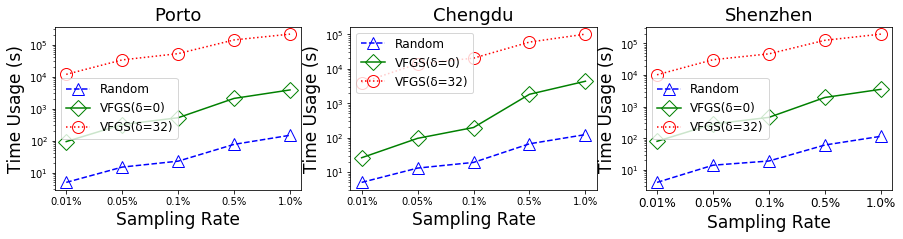
\includegraphics[width=0.5\textwidth]{pictures/quantitative_study_icde/sample_time.png}
%	\vspace{-8mm}
%	\caption{Time usage vs. sampling rates.}
%	\label{fig:sample_time}
%	\vspace{-3mm}
%\end{figure}

%\begin{figure}
%	\centering
%	\small
%	\begin{tabular}{cc}
%		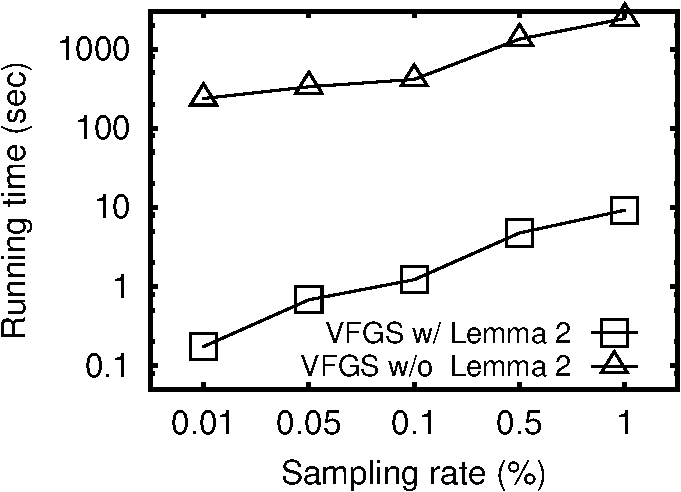
\includegraphics[width=0.44\columnwidth]{pictures/tporto}
%		&
%		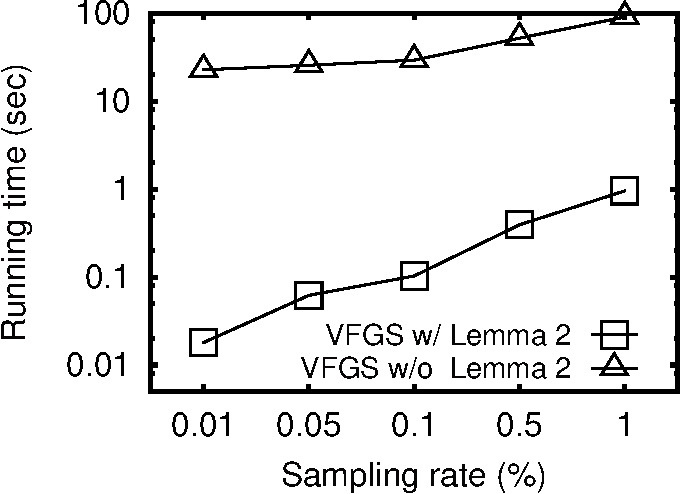
\includegraphics[width=0.44\columnwidth]{pictures/tshenzhen}
%		\\
%		(A) \pt{}
%		&
%		(B) \sz{}	
%	\end{tabular}
%	\vspace{-3mm}
%	\caption{Running time of $\vats$ w/ and w/o Lemma~\ref{lem:submodular}.}
%	\label{fig:cost}
%	\vspace{-6mm}
%\end{figure}
%\QM{unfininshed}
%We first conduct an experiment to evaluate the rendering cost by datasize. We vary the number of trajectories from 1000 to 1 million, which are randomly selected from \pt{} dataset. The experimental results are summarized in Table~\ref{tab:gpu}. We observe that the rendering cost is linear with the input data trajectories.
%
%We first report the running time of our $\vats$ algorithm in Figure~\ref{fig:cost} by varying the sampling rate from $0.01\%$ to $1\%$. The results show that $\vats$ is quite slow without the submodularity of contribution value, which agrees with Lemma~\ref{lem:submodular} in Section~\ref{sec:opt}.
%Then we shown the total time usage with sampling rate as Figure~\ref{fig:sample_time}. {*******}
%
%The optimized $\vats$ (e.g., $\vats$ with Lemma~\ref{lem:submodular}) outperforms $\vats$ by one to three orders of magnitudes on both datasets. The result show that running time of our $\vats$ algorithm is below 1 second in most cases. We have shown that $\vats$ provides good visualization performance with a low sampling rate (e.g., $0.1\%$ or $1\%$) in Section 6.1 and 6.2,  and Table~\ref{tab:gpu} suggests that the rendering latency scales almost linearly with dataset cardinality. By significantly reducing the dataset cardinality with sampling, $\vats$ can effectively reduces the rendering latency to make interactive visualization possible without sacrificing visual quality. For example, rendering the full $\pt{}$ dataset takes about \QM{34 seconds}, with a sampling rate of $1\%$, $\vats$ can bring down the rendering latency to less than 1 second.





\section{Conclusions}\label{sec:con}


This paper presents the $\avats$ framework, which achieves high visual quality and low visualization latency for large-scale trajectory datasets. $\avats$ provides guaranteed visual quality in trajectory sampling by formulating a quality optimal sampling problem and developing effective solutions including $\vats$ and $\vats$. Low visualization latency is achieved with the $\invQ$-tree index, which allows to use the sampling results computed offline. Experiment results show that $\avats$ consistently provides high quality visualization in different cases and its visualization time is orders of magnitude shorter than full visualization.
%We plan to extend $\avats$ to support the specific trajectory features such as mulit-class characteristics in the future. 

%a novel sampling technique, $\avats$, that guarantees the visual quality of line-based trajectory visualization and alleviates the visual clutter problem. The effectiveness and efficiency of the proposed method are validated with real world visual analysis tasks and quantitatively performance measurements. Possible future directions include (i) improving visual quality by sampling trajectory segments instead of complete trajectories and (ii) developing advanced color encoding schemes to better describe the spatial distribution of the trajectories.
%extending our approaches to support the specific trajectory features such as mulit-class characteristics.

%we focus on the sampling approach of trajectory segments other than the whole trajectories to achieve higher visual fidelity.
%We will also develop different color encoding schema to present the spatial distribution of trajectories more precisely. Currently, the color of one trajectory keep the same, thus the color of the long trajectories may mislead the users because they may pass through many regions with different traffic crowdedness.
%We also consider to extend our approach to support the specific trajectory features such as mulit-class characteristics. 
%%
%% The acknowledgments section is defined using the "acks" environment
%% (and NOT an unnumbered section). This ensures the proper
%% identification of the section in the article metadata, and the
%% consistent spelling of the heading.
% \begin{acks}
% To Robert, for the bagels and explaining CMYK and color spaces.
% \end{acks}

%%
%% The next two lines define the bibliography style to be used, and
%% the bibliography file.
\bibliographystyle{ACM-Reference-Format}
\bibliography{ref}

%%
%% If your work has an appendix, this is the place to put it.
% \appendix
% \section{Research Methods}
% \subsection{Part One}

% Lorem ipsum dolor sit amet, consectetur adipiscing elit. Morbi
% malesuada, quam in pulvinar varius, metus nunc fermentum urna, id
% sollicitudin purus odio sit amet enim. Aliquam ullamcorper eu ipsum
% vel mollis. Curabitur quis dictum nisl. Phasellus vel semper risus, et
% lacinia dolor. Integer ultricies commodo sem nec semper.

\end{document}
\endinput
%%
%% End of file `sample-authordraft.tex'.
